\documentclass[degree=master]{thuthesis}
% 选项:
%   degree=[bachelor|master|doctor|postdoctor], % 必选
%   secret,                                     % 可选
%   pifootnote,                                 % 可选(建议打开)
%   openany|openright,                          % 可选,基本不用
%   arial,                                      % 可选,基本不用
%   arialtoc,                                   % 可选,基本不用
%   arialtitle                                  % 可选,基本不用

% 所有其它可能用到的包都统一放到这里了,可以根据自己的实际添加或者删除。
\usepackage{thuthesis}

% 定义所有的图片文件在 figures 子目录下
\graphicspath{{figures/}}

% 可以在这里修改配置文件中的定义。导言区可以使用中文。
% \def\myname{薛瑞尼}

\begin{document}

%%% 封面部分
\frontmatter
\thusetup{
  %******************************
  % 注意:
  %   1. 配置里面不要出现空行
  %   2. 不需要的配置信息可以删除
  %******************************
  %
  %=====
  % 秘级
  %=====
  secretlevel={秘密},
  secretyear={10},
  %
  %=========
  % 中文信息
  %=========
  ctitle={高性能用户态协议栈的\\兼容性研究},
  cdegree={工程硕士},
  cdepartment={计算机科学与技术系},
  cmajor={计算机技术},
  cauthor={姜惠友},
  csupervisor={李~~~丹副教授},
  % 日期自动使用当前时间,若需指定按如下方式修改:
  % cdate={超新星纪元},
  %
  % 博士后专有部分
  cfirstdiscipline={计算机科学与技术},
  cseconddiscipline={系统结构},
  postdoctordate={2009年7月——2011年7月},
  id={编号}, % 可以留空: id={},
  udc={UDC}, % 可以留空
  catalognumber={分类号}, % 可以留空
  %
  %=========
  % 英文信息
  %=========
  etitle={Research on Compatibility of High-performance Userspace Protocol Stack},
  % 这块比较复杂,需要分情况讨论:
  % 1. 学术型硕士
  %    edegree:必须为Master of Arts或Master of Science(注意大小写)
  %             “哲学、文学、历史学、法学、教育学、艺术学门类,公共管理学科
  %              填写Master of Arts,其它填写Master of Science”
  %    emajor:“获得一级学科授权的学科填写一级学科名称,其它填写二级学科名称”
  % 2. 专业型硕士
  %    edegree:“填写专业学位英文名称全称”
  %    emajor:“工程硕士填写工程领域,其它专业学位不填写此项”
  % 3. 学术型博士
  %    edegree:Doctor of Philosophy(注意大小写)
  %    emajor:“获得一级学科授权的学科填写一级学科名称,其它填写二级学科名称”
  % 4. 专业型博士
  %    edegree:“填写专业学位英文名称全称”
  %    emajor:不填写此项
  edegree={Master of Engineering},
  emajor={Computer Technology},
  eauthor={Jiang Huiyou},
  esupervisor={Professor Li Dan},
  % eassosupervisor={Chen Wenguang},
  % 日期自动生成,若需指定按如下方式修改:
  % edate={December, 2005}
  %
  % 关键词用“英文逗号”分割
  %ckeywords={\TeX, \LaTeX, CJK, 模板, 论文},
  %ekeywords={\TeX, \LaTeX, CJK, template, thesis}
}

% 定义中英文摘要和关键字
\begin{cabstract}
随着移动互联网和人工智能的迅猛发展,不仅网络数据中心的整体流量与日俱增,而且由于RPC、HTTP、KV存储等业务的重要性不断提升导致小包数据占整个网络流量的比重越来越高。此外,随着硬件设备的迭代升级,40Gb、100Gb等高吞吐硬件网卡已经逐渐在数据中心广泛部署,传统网络内核协议栈作为底层网络传输网卡与上层网络应用之间的沟通桥梁,开始严重拖慢数据中心的网络性能。近几年工业界和学术界主要有在内核态和用户态对网络协议栈进行优化的两种研究途径,在内核态调优协议栈由于无法完全避免系统调用带来的开销造成性能提升有限,而在用户态实现的高性能协议栈普遍存在着兼容性差、移植成本高的问题,至今依然没有出现一款在保证网络性能明显提升的前提下达到网络应用高度兼容的协议栈系统。

本文针对当前高性能网络协议栈普遍存在着传统应用移植代价高、编程接口复杂的问题,在高性能用户态协议栈的兼容性方面进行研究、设计与实现,使得传统应用在完全不需要修改任何源码的情况下就能得到网络性能的提升。该协议栈基于DPDK高速轮询IO收发包框架,并将Linux内核网络协议栈源码搬离到用户态实现,通过LD\_PRELOAD动态链接技术、文件描述符空间重映射机制和并发流CPU资源调度模块等解决种类繁多的网络模型的兼容性问题,同时协议栈进程与应用进程采用分核设计并分别进行分组绑定、绕过内核减少系统调用等设计也让网络应用兼具用户态协议栈的高性能优势。在兼容性方面,本协议栈既支持常见的POSIX网络API和Epoll IO多路复用相关接口,又能支持read、epoll\_wait等相关接口对非网络文件描述符的调用,还能兼容多进程、多线程等各种主流网络编程模型。此外开发了对协议栈进程和网络worker子进程进行监控的模块,当进程异常退出时候能回收文件描述符、socket结构体等资源,提升协议栈系统的鲁棒性。

Nginx、Lighttpd、Redis等主流网络应用已经被移植到该用户态协议栈。实验结果表明,在完全不需要修改源码的前提下,该协议栈为Nginx、Lighttpd应用带来30\%~60\%网络吞吐上的提升,减少近一半的平均延迟,同时将尾延迟大幅降低到原来的四十分之一。


\end{cabstract}

% 如果习惯关键字跟在摘要文字后面,可以用直接命令来设置,如下:
\ckeywords{兼容性;用户态协议栈;高性能}

\begin{eabstract}
With the rapid development of mobile Internet and artificial intelligence, not only the overall network traffic in data centers is increasing, but also the proportion of small packet in the entire network traffic soars due to the growing importance of services such as RPC, HTTP, and KV storage. On top of that, with the continual upgrade of hardware devices, 40Gb, 100Gb and other high-throughput NICs have been widely deployed in the data center. The traditional kernel protocol stack serving as a bridge between the underlying network transmission medium and the upper-layer network applications begins to seriously slow down network performance in the data center. In recent years, there are two research approaches in the industry and academia to optimize the network protocol stack, either in kernel space or user space. The performance improvement of optimization in kernel space is limited due to the inability to completely avoid system calls. And the user-space high-performance protocol stacks generally are poor in compatibility and high at transplantation cost. So far, there is no protocol stack system with both high-compatibility and high-performance.

In this paper, in order to address the issues of high transplantation cost and complicated programming interface in the state-of-the-art network protocol stack, the compatibility of high-performance user-space protocol stack has been researched, designed and implemented, that is, without any modification of source codes legacy applications can attain significantly improved network performance. The protocol stack is based on the DPDK high-speed polling IO packet processing framework, and shifts up the Linux kernel source codes of network function to the user space. The compatibility issue of variety in network programming models has been solved by LD\_PRELOAD dynamic link technology, file descriptor space remapping mechanism and concurrent stream CPU resource scheduling module. In addition, with seperation design between protocol stack process and application process, bypassing the kernel to reduce system calls, the high-compatibility protocol stack also retain the advantage of high performance in user-space. In terms of compatibility, the protocol stack supports both common POSIX network APIs and Epoll IO multiplexing related interfaces, as well as read, epoll\_wait and other related interfaces with non-network file descriptor input parameter, and it is compatible with multi-processes and multi-threads of mainstream applications. In addition, a module for monitoring the protocol stack process and the application process has been developed. When the application process exits abnormally, resources such as file descriptors and socket structures can be recycled, and the robustness of the protocol stack system has been improved.

Major network applications such as Nginx, Lighttpd, and Redis have been transplanted onto the user-space protocol stack. The experimental results show that with no modification of source codes, the protocol stack brings 30\%$\sim$60\% network throughput improvement for Nginx and Lighttpd Web applications, cuts down the average latency by nearly half, and dramatically reduces the tail latency to fortieth.

\end{eabstract}

\ekeywords{compatibility; user-space protocol stack; high performance}

% 如果使用授权说明扫描页,将可选参数中指定为扫描得到的 PDF 文件名,例如:
% \makecover[scan-auth.pdf]
\makecover

%% 目录
\tableofcontents

%% 符号对照表
\begin{denotation}[3cm]
\item[TCP] 传输控制协议  (Transmission Control Protocol)
\item[UDP] 用户数据报协议  (User Datagram Protocol) 
\item[HTTP] 超文本传输协议  (HyperText Transfer Protocol)
\item[API] 应用程序编程接口 (Application Programming Interface)
\item[FD] 文件描述符 (File Descriptor)
\item[VFS] 虚拟文件系统 (Virtual File System)
\item[TLB] 页表缓存 (Translation Lookaside Buffer)
\item[POSIX] 可移植操作系统接口 (Portable Operating System Interface)
\item[SO] 共享对象 (Shared Object)
\item[DPDK] 数据平面开发套件 (Data Plane Development Kit)
\item[RSS] 接收端扩展 (Receive Side Scaling)
\end{denotation}



%%% 正文部分
\mainmatter
\chapter{引言}
\label{cha:intro}

\section{研究背景}
\label{sec:01_general_intro}

互联网早期网络环境简单,设备带宽资源有限,基于Best-effort服务原则并受限于滑动窗口流量控制机制和TCP拥塞控制算法的网络协议栈足够满足当时需求。然而随着移动互联网的快速发展和人工智能海量数据处理中底层大规模分布式机器学习框架的兴起,这不仅使得数据中心的网络流量飞速增加,而且对网络处理的延迟和吞吐都提出更严苛的要求。在当今短视频、微博、游戏等各种业务的蓬勃发展,网络流量中HTTP、RPC等常见通信协议存在着大量的TCP短连接已经让网络协议栈有些不堪重负,TCP短连接意味着在三次握手、四次挥手这些复杂的TCP交互之中仅传递少量有效网络数据。根据相关调查显示,在较大规模的蜂窝网络中,有达到90\%的TCP流量是小于32KB,甚至小于4KB的TCP流也有超过一半之多~\cite{woo2013comparison},这无疑对数据中心中宝贵的CPU资源造成巨大浪费。

与此同时,在硬件设备方面,随着40Gb、100Gb乃至200Gb带宽的硬件网卡设备逐渐部署,以及CPU经历摩尔定律的主频指数增加之后又开始往多核架构方向发展,并且DDR3、DDR4高速物理内存和固态硬盘等设备逐渐应用在高速网络数据中心中,迭代缓慢的传统内核网络协议栈已经难以跟上硬件设备的更新以及网络流量的飞速发展,这使得网络性能瓶颈的压力又转移到软件层面的传统内核网络协议栈上。

所以,加速网络协议栈就成为如今整体提升网络性能的重中之重。最近几年在该领域的研究可以大体归为三类。第一类研究方向是将网络协议栈向下offload到硬件设备网卡,比如通过RDMA网卡彻底绕过CPU和内核从而实现极致的网络性能提升,但此路径依赖硬件设备并且仅适用于超高网络性能要求的专用场景,完全不具备对网络应用的兼容性;第二类在内核态对现有内核网络协议栈进行调优,该方式由于无法完全避免系统调用带来的开销并且难以利用高速IO收发包框架从而造成网络性能提升有限;第三类是将协议栈完全搬离到用户态来实现,这在绕过内核和高速IO框架等优化方式下确实可获得显著的性能提升,不过移植传统网络应用通常还需要修改应用源码。这三条路径本殊途同归,最终都是为了减少网络协议栈对整个系统的开销从而提升网络应用的服务性能指标,然而过分追求网络性能的提升而忽略协议栈本身的兼容性会导致移植传统网络应用成本过高等兼容性问题。此外,由于在硬件网卡中加速网络协议栈初衷仅适用于专用场景,所以我们在后续第二章中仅对后两条路径做更加详细的说明。

TCP/IP协议栈最初作为操作系统的一部分,在Unix、Linux、Solaris、FreeBSD等各个系统中都有实现,为了能让网络应用可以直接运行在众多系统,各个网络协议栈向上层网络应用暴露服务接口时候都必须符合POSIX标准,这为后来互联网的飞速发展提供了扎实的技术基础。近几年影响力较大的用户态高性能网络协议栈mTCP~\cite{mTCP}由于移植网络应用需修改其源码导致从发布至今四年多时间里只成功移植Lighttpd这一款主流的网络服务器应用,而内核态网络协议栈Fastsocket~\cite{fastsocket}虽然性能提升没有mTCP明显但因具备高度应用兼容性已经部署到新浪微博的生产环境中。从中不难看出兼容性对高性能网络协议栈的后续发展至关重要。

在上述背景下,本文在用户态基于高速轮询IO DPDK~\cite{DPDK}框架设计并实现了高度兼容的网络协议栈,通过LD\_PRELOAD动态链接技术、文件描述符空间重映射机制和并发流CPU资源调度模块等解决种类繁多的网络模型的兼容性问题,在保证用户态协议栈网络性能提升明显的前提下,实现了高度兼容性,即传统网络应用在不需要修改任何源码的情况下即可直接移植到该协议栈上获得网络性能的提升,几乎达到移植零成本。

\section{研究问题及其意义}
\label{sec:01_problem_intro}
本文针对当前网络协议栈的兼容性普遍较差、需要修改网络应用源码才能获得网络性能提升的问题,设计并在用户态实现一款兼具高性能的同时可以完全不需要修改网络应用源码即可完成移植的高度兼容的网络协议栈,这样为开发人力资源紧张的中小型企业几乎零成本地带来网络性能的提升。本文重点要解决的问题是如何完成对基于多进程、多线程、Epoll IO多路复用等网络编程模型的众多网络应用进行支持,并且要保证能在不需要修改网络应用源码前提下即可完成移植。此外,网络协议栈想要推广也必须有较为明显的网络性能提升,这就需要协议栈在设计之初就利用高速IO收发包框架绕过内核、并在多个进程或线程同时运行的情况下合理地完成对CPU资源的调度与分配,通过合理且高效的数据结构来完成进程间通信。

当前学术界已经有不少高性能用户态协议栈为网络应用带来显著的性能提升~\cite{mTCP,IX,ZygOS},然而过度追求高性能,尤其是向网络应用暴露硬件网卡收发包的控制细节虽然会带来一定的性能提升,但导致协议栈的接口脱离传统的POSIX API语义,对网络应用开发人员十分不友好。这种高性能用户态协议栈大多仅适用于对网络性能指标要求极高的专用网络场景,但是想将其推广到各种传统网络应用对开发人员将是十分棘手的事情。

所以对网络应用高度兼容的网络协议栈的意义十分明确,就是在可以不需要修改网络应用源码的前提下,零成本地完成对多进程、多线程、Epoll等各种主流网络应用的移植,并带来较为明显的网络性能提升。

\section{研究难点与挑战}
\label{sec:01_difficulties_and_chanllenge}
本文的研究难点主要分为以下几个方面:

第一,就是如何在不修改传统网络应用的源码的前提下完成对基于多种网络编程模型的传统网络应用的支持,其中既要支持常见的socket、bind、listen、accept、read、write等网络函数,也要支持Epoll这种高效的IO多路复用机制,还要对shutdown、dup、dup2等这些并不常见但也偶尔出现于主流网络应用的接口进行支持。与此同时,完成对这些POSIX API系统调用的劫持,并能最大程度保留read、write、epoll\_wait这些函数对非网络文件描述符的支持。

第二,在用户态实现网络协议栈的同时并保证协议栈功能的完整性、鲁棒性与安全性,本文基于Linux内核3.14.2版本将其网络协议栈功能部分剥离出来,这需要在熟练掌握内核协议栈实现的基础上去划分网络功能的边界,并用高速IO收发包模块的底层开发套件替换掉内核协议栈中网卡netdev、内存管理、定时器等边界函数,具有较高的技术挑战。

第三,协议栈运行过程中可能存在多个进程或线程同时运行于系统中,包括协议栈进程、网络应用进程等,如何将这些并发流在有限的CPU核资源上合理进行分配与调度,在尽可能最大化利用CPU资源的同时尽量减少或避免对CPU资源的严重竞争,这对于多进程应用的网络性能也尤为重要,并且在用户态完成该工作也具备一定技术挑战。

\section{论文结构安排}
本文由六个章节组成,主要内容分别如下。

第一章概括性地介绍高性能网络协议栈兼容性的研究背景,并指出本文的研究内容、研究意义与研究挑战。

第二章从内核态和用户态两个方面介绍高性能协议栈的相关研究工作,并详细地介绍几款经典的高性能协议栈的系统架构与实现以及存在的问题,并与本文工作进行对比分析,突出本工作的研究挑战与意义。

第三章介绍该用户态协议栈在兼容性方面的设计,其中会先对协议栈系统的整体架构进行介绍,包括协议栈与网络应用的分核设计理念与进程间通信的设计,接下来会重点介绍协议栈在兼容性方面的设计,其中包括通过LD\_PRELOAD动态链接技术完成对POSIX网络API的劫持、通过文件描述符空间重映射完成对网络文件描述符与非网络文件描述符的分割管理、用户态Epoll IO多路复用机制的实现、并发流网络模型的的设计与实现、以及系统异常崩溃时进行资源回收等的设计,从而实现网络应用的高度兼容性。

第四章对该用户态协议栈兼容性方面的实现进行详细介绍,包括进程间通信消息结构的设计,socket和文件描述符等关键资源的数据结构的设计与优化以及各种网络接口的具体实现方案。

第五章对已经成功移植的主流网络应用Nginx、Lighttpd、Redis以及独立开发的一款多线程Epoll网络服务器进行实验性能方面的评估并与最新版本的Linux内核进行对比。

第六章对本文的研究工作成果进行总结,并为网络协议栈兼容性更进一步的设计提供展望。


\chapter{研究背景和相关工作}
\label{cha:02_related_work}
本章的内容主要从两个方面对网络协议栈相关工作进行详细介绍,第一方面是在内核态直接对网络协议栈进行调优,第二方面是将网络协议栈搬离到用户态实现并进行更深度的优化。此外,对两种方式的优劣分别进行分析,并与本工作进行对比。

\section{内核态网络协议栈的优化工作}
\label{sec:02_kernel}

\subsection{Linux内核网络协议栈优化}
网络协议栈诞生初期就一直作为内核操作系统的一部分,毕竟数据包处理涉及到网卡硬件资源的管理,为了保证安全需要操作系统的内核态权限才能对硬件网卡直接进行操作。早在上个世纪八十年代,协议栈从内核分离出到用户态的想法就已经被提出~\cite{1987packer},但是由于在用户态进行数据包多路复用产生过多的上下文切换以及进程间通信的开销,所以当时的背景下在内核态实现实现协议栈有着更高的网络性能。

操作系统内核在不断演进中也为网络协议栈的优化做出不可磨灭的贡献。早期的TCP/IP协议栈存在着严重的多核扩展性问题,这主要因为多核共享资源的锁竞争造成的开销,如图\ref{fig:accept_queue_lock}所示,为了支持更多的并发,网络应用常常在多个核上开启多个并发流同时监听同一个listen socket,为了保证并发安全内核在共享的accept队列等全局资源中加入锁,这样在大量网络并发时候会造成严重的锁资源竞争开销,导致较差的多核扩展性,甚至造成随着CPU核数的提升,网络性能反而变得更差。

在内核中为了解决该问题,在Linux内核3.9版本中SO\_REUSEPORT~\cite{SO_REUSEPORT}选项被引入进来,该关键字使得不同socket可以绑定在同一个网络端口。如图\ref{fig:accept_queue_unlock}显示的是引进SO\_REUSEPORT后监听的工作模式,本质上就是将accept队列这个原来全局共享的资源拆分到每个核的每一个socket,减少锁资源的竞争开销。不过该功能需要应用程序在调用socket函数时候添加SO\_REUSEPORT作为参数,对用户并不透明,所以兼容性并不是好。

% \vspace{-10pt}
\begin{figure}[htbp]
\centering
\begin{minipage}[t]{0.48\textwidth}
\centering
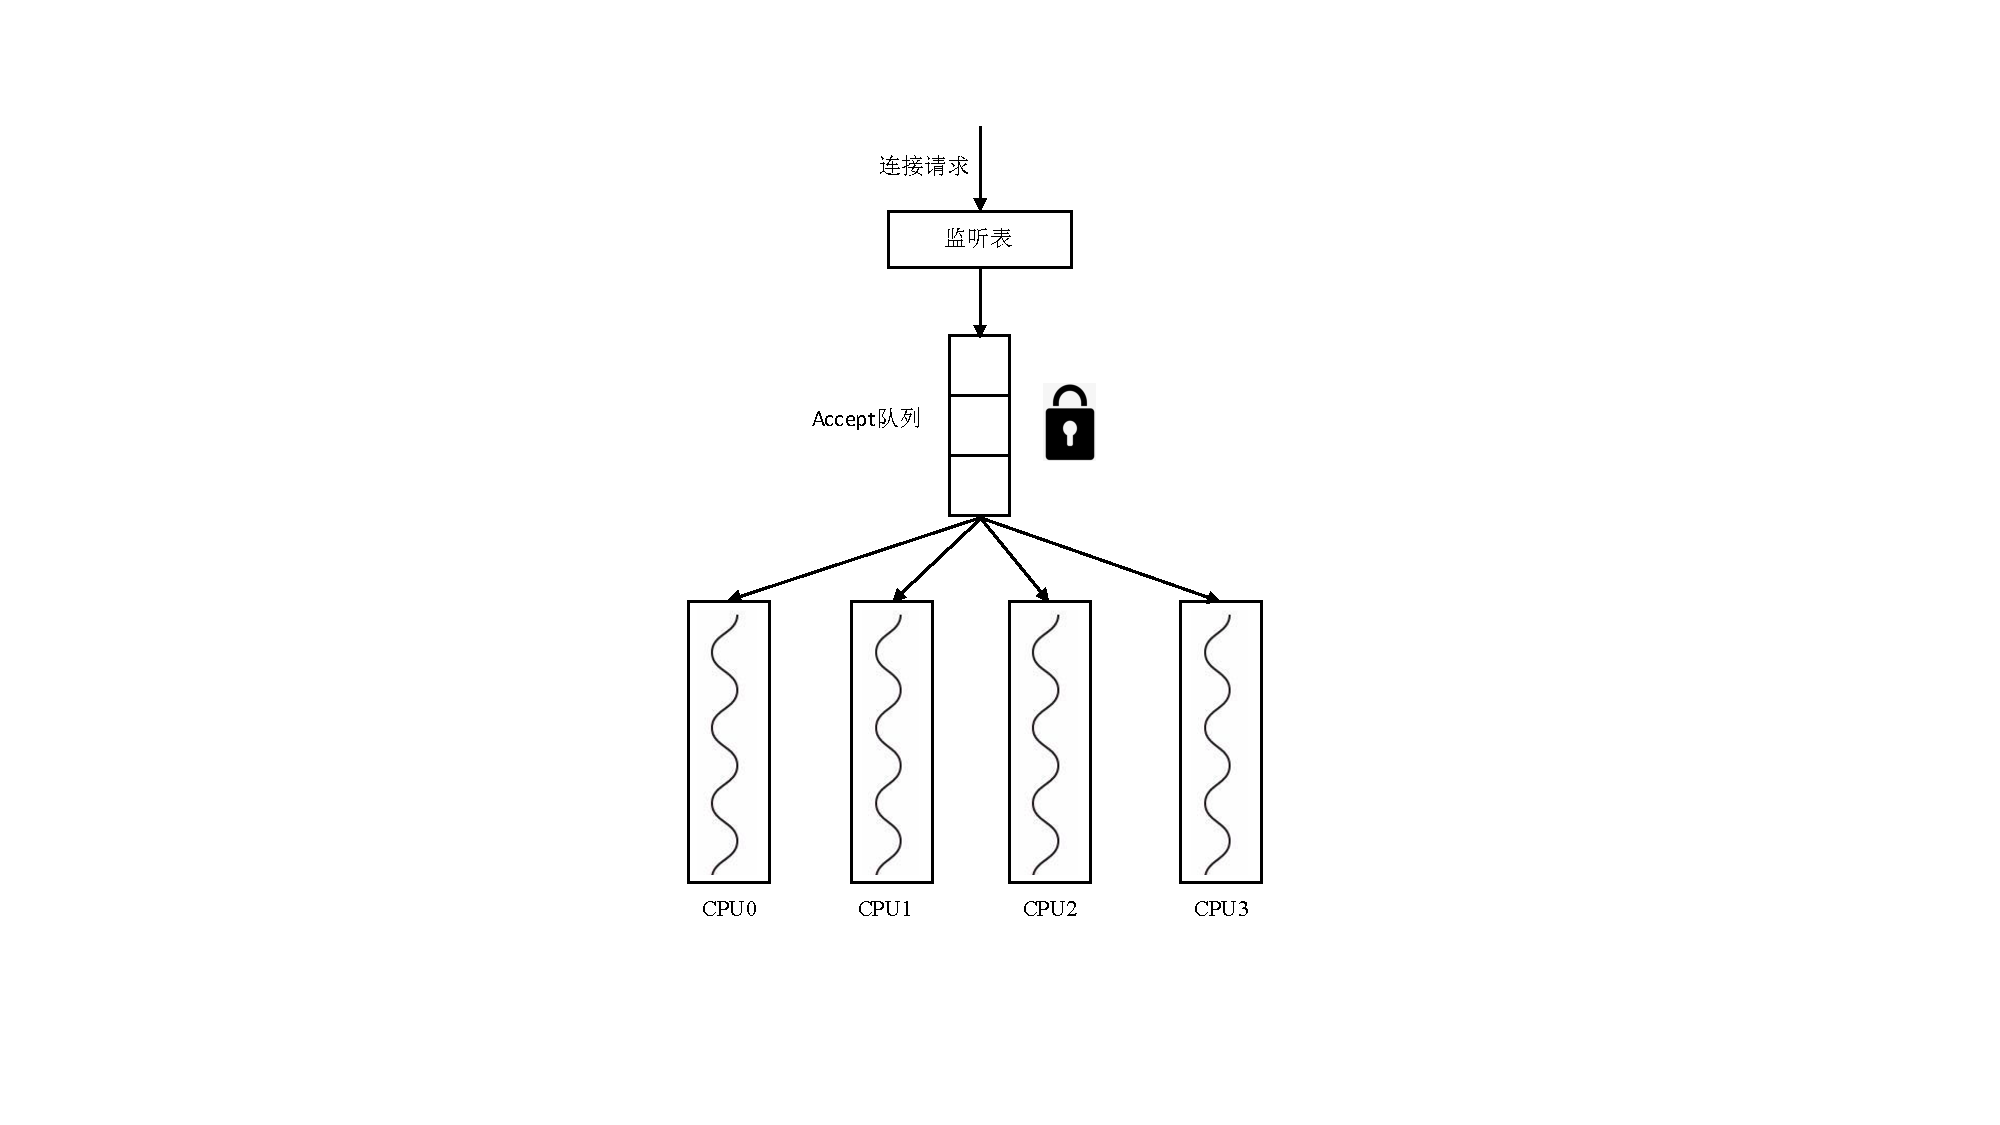
\includegraphics[width=6cm]{accept_queue_lock.pdf}
\caption{SO\_REUSEPORT引入之前}
\label{fig:accept_queue_lock}
\end{minipage}
\begin{minipage}[t]{0.48\textwidth}
\centering
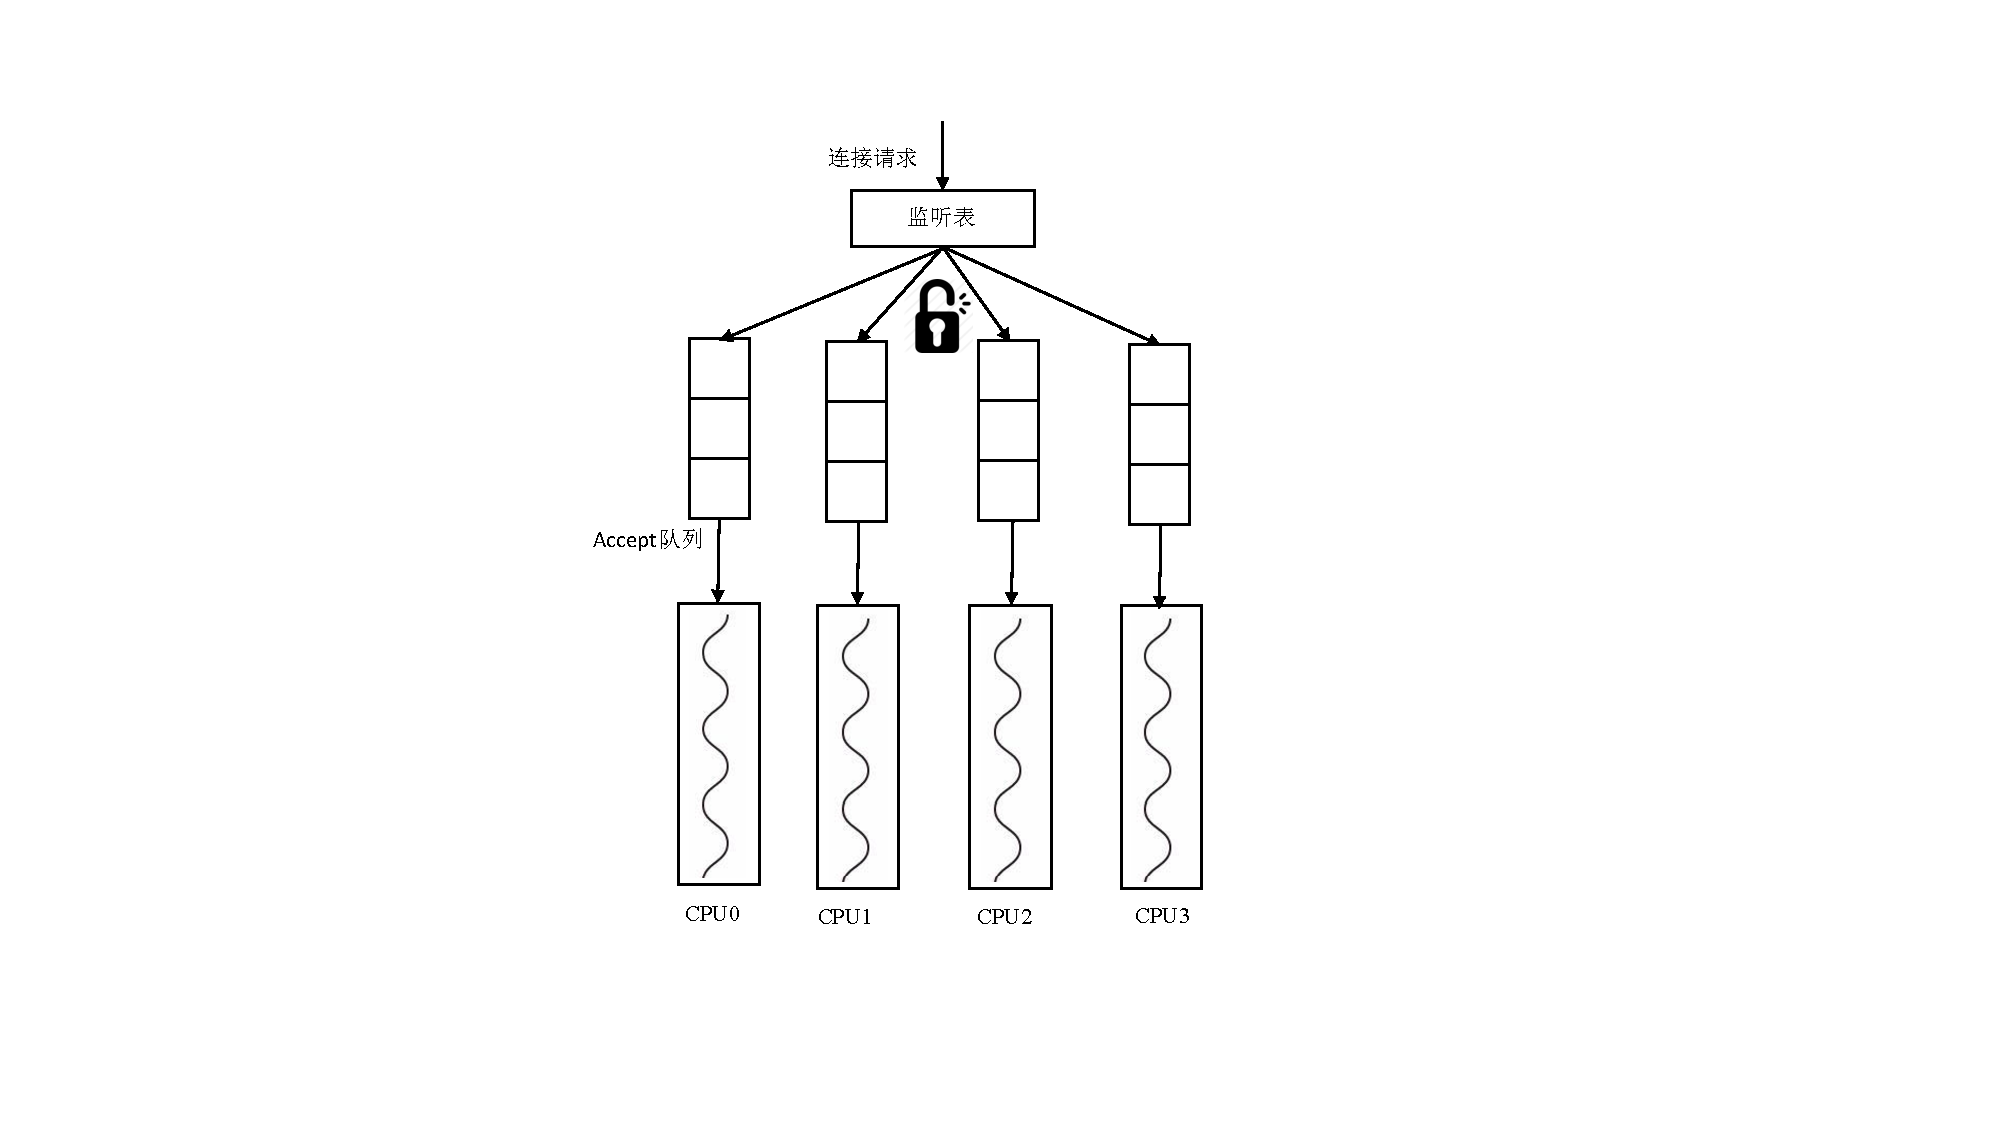
\includegraphics[width=6cm]{accept_queue_unlock.pdf}
\caption{SO\_REUSEPORT引入之后}
\label{fig:accept_queue_unlock}
\end{minipage}
\end{figure}
% \vspace{-10pt}

对于使用IO多路并发的服务器,比如Nginx中使用epoll,当多个并发流监听同一个listen socket存在着惊群现象,即多个执行流均在调用epoll\_wait函数发生阻塞,当一个新网络连接到达时,内核会唤醒所有执行流,但只有其中一个能真正接收该连接并进行数据传递,这在网络吞吐并不高的环境下无效的唤醒造成CPU等资源的浪费。Linux4.5版本中引入EPOLLEXCLUSIVE选项~\cite{EPOLLEXCLUSIVE}解决了Epoll惊群问题,但同样需要在调用epoll\_ctl函数时候添加该选项才能生效,对用户的兼容性也并不友好。
对网络协议栈中数据拷贝的优化在内核中也不断发展,sendfile是通过网络向远端发送本地磁盘文件的接口,它的出现减少了内核态与用户态之间的两次数据拷贝,但是由于该接口仅能应用于文件,并不支持socket之间的网络通信,对网络性能的提升有限,此外它并不属于POSIX或其他任何标准中,在各个操作系统中实现并不统一。在Linux4.14版本中采纳MSG\_ZEROCOPY~\cite{msg_zerocopy}选项来实现数据的零拷贝,该实现是基于虚拟化技术tuntap~\cite{tuntap}、vhost和xen~\cite{Xen}的零拷贝框架。然而该功能的生效既需要调用setsockopt函数为该socket设置SOCK\_ZEROCOPY选项,还需要在接收或发送的函数参数中加入MSG\_ZEROCOPY,应用兼容性更加不好。

从上面的介绍可以看出,操作系统内核对协议栈的优化虽然没有改变POSIX API本身,但还是需要用户修改网络应用源码,并且对网络性能的提升幅度有限。而发展缓慢的内核已经跟不上互联网流量膨胀的速度,于是大量从内核态对协议栈进行深度调优的工作不断涌现出来。

\subsection{内核态调优网络协议栈}

传统的网络协议栈无法保证在一个TCP连接整个过程,包括接收数据、内核TCP状态机处理、用户态代码执行、内存分配、发送数据这些阶段都只在一个核上进行,例如图5所示,数据接收以及三次握手建连的逻辑由CPU0来完成,但发送数据时候却由CPU2进行,在这种情况下跨核Cache数据的迁移造成CPU中Cache和TLB的Miss概率提升进而影响协议栈的整体性能。为了解决该问题,Affinity-Accept~\cite{Affinity-Accept}基于2.6.35版本的Linux内核通过accept队列本地化、减小连接Hash映射表锁的粒度等优化保证一个TCP连接全过程只在一个CPU核进行,实验显示,该优化在单核中降低30\%的TCP协议栈处理时间并提升24\%的整体网络吞吐。由于该优化是直接在Linux内核中并且完好地保持POSIX网络API,所以该方案理论上具备高兼容性,只不过对网络系统的提升有限。

作为同年发表的研究成果,MegaPipe~\cite{MegaPipe}在内核态对协议栈进行更大规模的优化,这是由于在面向消息的应用中,比如HTTP、RPC、DB、Key-value Store中,要么一个TCP连接传递的数据量较少,要么TCP连接时间较短,这些网络流量对服务器CPU资源是隐形杀手,毕竟CPU cycle的时间不少浪费在TCP三次握手和四次挥手这些网络逻辑中。MegaPipe的主要优化点如下:

\begin{enumerate}[(1),labelsep=.5em, leftmargin = 0pt, itemindent = 3em]
\item 通过在内核网络API与网络应用之间建立系统调用批处理的channel以最大程度降低网络系统调用引发上下文切换带来的开销。
\item 对listen socket中accept队列与hash建连表等资源进行本地化处理,与Affinity-Accept中优化相似。
\item 将虚拟文件系统VFS从网络socket中剔除,设计出更轻量级的socket API。
\end{enumerate}

文章实验结果显示这些优化与原内核网络协议栈相比在memcached中带来超过15\%的性能提升以及在Nginx中带来75\%左右的性能提升。然而,MegaPipe并不具备任何兼容性,因为其设计一套完全不同于原POSIX网络API的接口使其难以应用到众多网络应用中,再加上其并没有将源代码开源,也就使得它最终停留在实验室阶段。

socket接口中系统调用开销在另一篇文章~\cite{hruby2014sockets}得到更全面的分析,由于用户态陷入到内核态涉及到的安全权限的切换以及对CPU Cache、分支预测器、TLB等资源的污染,系统调用的开销也是不容忽视。尤其针对read、write、accept、select等这些在一次TCP连接中会被反复调用的接口,与MegaPipe重新设计网络API的策略相反,该文章通过将socket缓存暴露到网络应用等手段使得在网络高负载情况下消除99\%的系统调用开销,并将其用户加速基于微内核多服务器的系统NewtOS~\cite{hruby2012keep}。这种策略确实使其具备高度的兼容性,网络应用完全不需要修改源码即可运行在系统调用经过优化的POSIX网络接口上。然而该文章并没有明确阐述其与其他研究成果哪怕是Linux内核的性能对比。

Fastsocket~\cite{fastsocket,fastsocket-release}是最新对内核网络协议栈优化的研究成果,它在研究之初就是为了将系统最终落地到业界真实生产环境中,这就带来一些性能以外的考量,首先就是兼容性,包括网络API的兼容性、符合RFC规范、可以应用在主流常见网卡中,因为公司的网络服务众多,研发成本或硬件成本较大可能很难在公司中推广;此外还有协议栈的安全性,能抵御各种各样常见的网络攻击,如DDos拒绝服务攻击、连接劫持攻击等。

\vspace{-10pt}
\begin{figure}[H] % use float package if you want it here
  \centering
  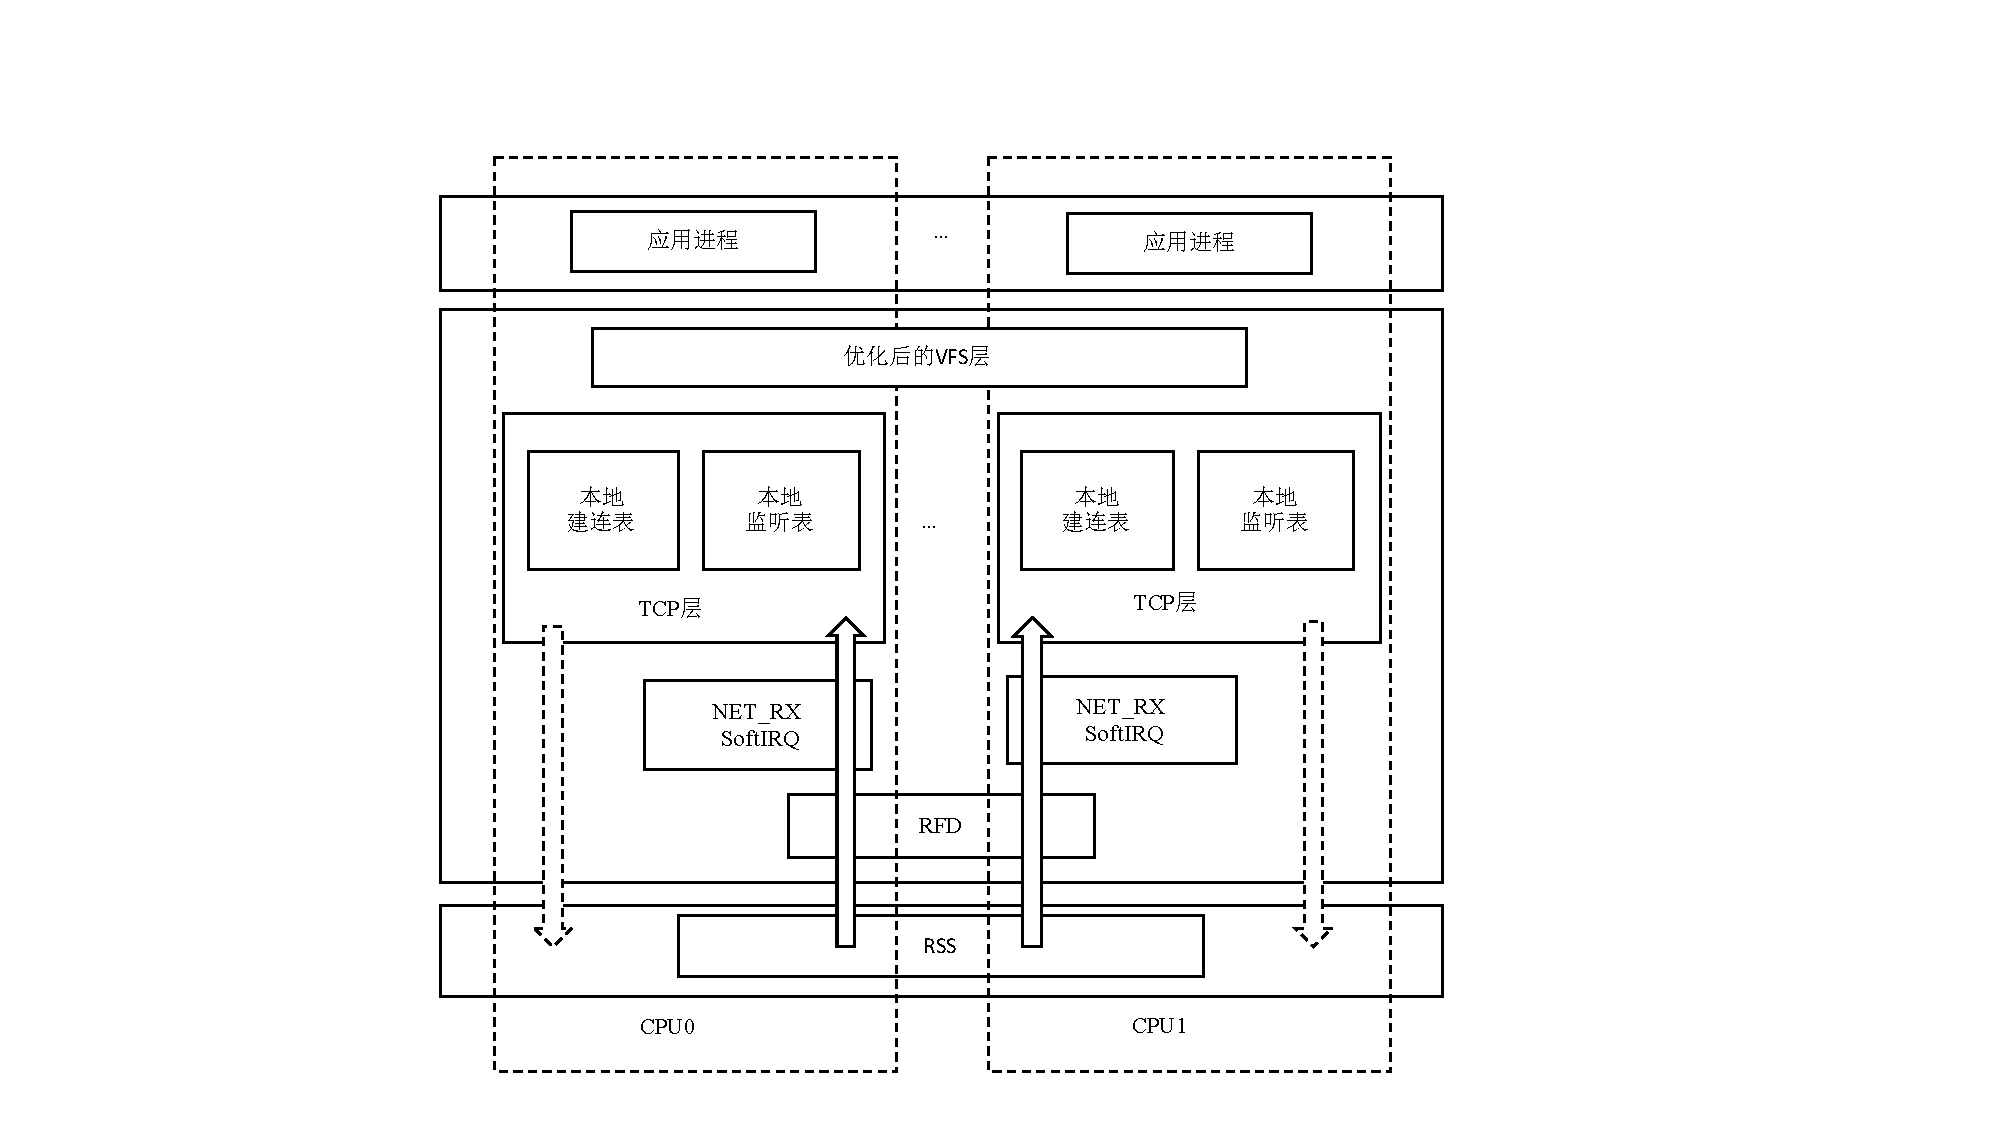
\includegraphics[width=\textwidth]{fastsocket}
  \caption{Fastsocket架构图}
  \label{fig:fastsocket}
\end{figure}
\vspace{-10pt}

基于以上的研究目的,Fastsocket在内核态对协议栈也是在TCP连接共享资源的拆分、虚拟文件系统VFS的优化、连接本地化这三方面进行更加彻底的优化。其系统架构图如图\ref{fig:fastsocket}所示,Fastsocket首先在底层通过RSS (Receive Side Scaling)和RFD(Receive Flow Deliver)来分别实现被动连接和主动连接的本地化,即网络服务不论是监听套接字接收连接还是调用connect函数发起连接,都可以保证整个TCP连接过程中仅发生在唯一一个CPU核上。被动连接直接根据网络请求的五元组计算CPU号来完成本地化,而对于更为复杂的主动连接,当网络服务调用connect主动发起连接 请求时,Fastsocket会依据该服务所在线程对应的CPU号计算出该网络连接的源端口号,而不是像传统内核一样随机产生,当该连接接收到对端的响应报文时候便根据该端口号逆向计算出对应的CPU号,之后就交给该CPU进行网络处理,如此反复进行,这样主动连接的整个TCP连接就都在唯一一个核上进行。连接本地化避免TCP数据在CPU之间跨核造成Cache、TLB Miss,从而提升了性能,此外它也为TCP建连表与监听表等资源按CPU级别拆分提供支持。Fastsocket中每一个core拥有自己独立的TCP建连表与监听表,一旦有新连接到来,通过RSS调度到某一CPU核后,协议栈会就会在该CPU 核运行一个内核线程来处理该连接,这样新建连接的TCP报文只需要在该CPU核中的建连表进行查询即可,避免并发流处理中锁同步竞争的开销,监听表也与此类似,也正是因为有连接本地化作为基础,不会存在后来的报文到达另外CPU核中而丢失TCP建连表信息的问题,这大大提升了协议栈的多核扩展性。



此外,Fastsocket也对VFS进行优化,因为据实验分析~\cite{boyd2010analysis},在流量负载较高且socket频繁申请的情况下,VFS花费不少时间去管理全局可见的inodes和dentries资源,去除socket在文件系统实现中inode\_lock这些对网络系统无关轻重的锁。实验结果显示Fastsocket在24核系统中实现了20.4倍相对于单核系统加速,多核扩展线性系数达到0.85,在Nginx和HAProxy网络应用中与Linux内核对比分别提升267\%和621\%之高。此外,更是因为其具备很好的兼容性,即不需要修改应用源码就可部署的低成本优势,使得其已经在新浪微博公司的真实生产环境中落地,从中不难看出兼容性对于网络协议栈能否真正被应用的重要性。

在内核中对协议栈进行优化在一定程度上可以保留Socket API,具备较好的兼容性,也能很好的解决原内核协议栈中多核扩展性的问题。不过由于数据在内核态与用户态的拷贝,传统基于中断的IO收发包模式的低效,难以完全避免的系统调用开销这种问题在内核态都难以得到解决,所以它带来的性能提升往往比较有限。此外,网络协议栈局限在内核中也会减缓其本身的发展速度,具有不方便调试等一系列问题。

\section{用户态优化网络协议栈}
\label{sec:userspace}
内核协议栈难以调试、发展受限等缺点在上个世纪八十年代就引起研究人员的注意,并不断尝试将协议栈搬离到用户态来实现,包括探索微内核网络架构~\cite{maeda1994protocol}、网络性能优化~\cite{thekkath1993implementing,basu1995user,edwards1995experiences}等,但都无法取得优于内核协议栈的网络性能。在当时上下文切换和跨进程间通信是实现用户协议栈两大性能障碍~\cite{1987packer},向各个网络应用进行packet demultiplex的任务如果放到进行用户态进程来做,相比于内核态实现就会造成过多次的上下文切换。究其根本原因,就是当时的技术背景还没有出现一种性能较高的绕过内核直接完成网络收发包的技术,这也是在用户态实现高性能网络协议栈的基础。


\subsection{绕过内核(Kernel Bypass)技术}
\label{subsec:02_dpdk}

Kernel Bypass最常见的实现方式是利用高速IO网络收发包框架,它们通常是经过一系列优化专为高吞吐网络流量环境设计。 IO虚拟化为协议栈网卡资源管理和绕过内核带来新的思路。SR-IOV为多虚拟机系统的高速IO共享同一物理网卡资源提供规范,一个带有SR-IOV~\cite{dong2012high}功能的物理网卡能被切分为多个独立的功能子模块,每一个功能模块都可以像一块独立的物理网卡为上层网络应用提供服务。Hypervisor软件去创建这些虚拟的功能模块,并在SR-IOV虚拟网卡中配置过滤规则去对数据包进行demultiplex,从而到达不同的网络协议栈。基于高速IO模块的网络应用性能通常要更好,但是会独占网卡使其无法收发内核协议栈数据包,而IO虚拟化可以与内核协议栈的网络通信共享同一物理网卡资源。此外,Rump Kernels~\cite{kantee2014rump}、User Mode Linux~\cite{dike2001user}也可以用来绕过内核直接在用户态运行应用,不过这些并不是针对网络协议栈设计,此文不予赘述。下面重点针对高速IO收发包模块这个在用户态协议栈中常用的技术进行展开介绍。
DPDK~\cite{DPDK}是Intel公司推出的一款高速处理数据包的框架,基于DPDK提供的包括收发包、定时器、内存管理等全套组件,网络应用可以完全与内核操作系统解耦来实现网络性能提升。根据其官网实验结果显示,在纯二层转发测试下,DPDK处理一个数据包仅需要80个CPU时钟周期,而CPU进行一次DRAM主存访问还需要上百个CPU周期。如此高的性能得益于如下几点优化:

\begin{enumerate}[(1),labelsep=.5em, leftmargin = 0pt, itemindent = 3em]
\item 大页内存管理其数据结构,其大小通常从2MB到数GB可灵活配置,而操作系统默认的内存页大小是4KB,这样可以大大减少TLB缓存Miss几率和缺页中断的发生。
\item 使用轮询替代中断的IO模式,在网络高负载情况下,中断收包模式下对CPU产生的硬件中断开销较大,轮询可以有效避免大流量时候频繁中断的开销。
\item 利用UIO网卡驱动实现Kernel Bypass,接收到的数据包直接可以在用户态进行处理,减少系统调用和数据包在内核态与用户态之间拷贝的性能开销。
\item RSS技术与亲核性机制将应用绑定在专门的CPU核中,减少数据跨核、Cache Miss带来的开销。此外,DPDK还利用CAS操作实现了一套无锁数据结构,例如rte\_ring等,这也减少锁带来的同步竞争开销。
\end{enumerate}

PF\_RING ZC (Zero Copy)~\cite{PF_RING}是在收发端均可实现1/10Gb线速转发的网络开发模块,当开启PF\_RING-aware driver时可以用来实现Kernel Bypass,从而减少系统调用开销。同时,PF\_RING ZC与其之前的版本都采用了内存预分配机制,并利用环形队列来实现内存资源的可重复利用,此外PF-RING ZC将用户态内存空间的地址映射到驱动的内存空间使得网络应用可以通过其API直接访问网卡的寄存器和内存数据从而实现了真正的零拷贝,然而这也为应用PF\_RING ZC编写网络应用程序带来因误操作网卡内存造成系统崩溃的安全隐患。

Netmap~\cite{NetMap}是一个高效的网络包处理模块,它通过数据包memory资源预分配减少每个数据包带来的内存分配的开销,利用网卡驱动buffer到用户态的内存映射技术实现零拷贝。Netmap的设计理念如图~\ref{fig:netmap}所示,当网络应用使用其接口接收数据时,网卡就与内核协议栈部分分离,使得数据可以绕过内核在共享内存中在网卡与应用之间进行传递,而对于传统操作系统的控制channel完全透明,OS的接口用来进行同步。所以严格来讲,Netmap在数据层面进行Kernel Bypass,而在控制层面依然依赖传统内核操作系统来完成信息传递。

高速IO收发包模块直接从网卡获得到二层数据裸包,在防火墙、流量监控等企业级服务器应用中使用较为方便,但要运行基于POSIX socket接口的网络应用,还需要独立的用户态网络协议栈对TCP/IP各层的网络逻辑进行实现。

\vspace{-10pt}
\begin{figure}[H] % use float package if you want it here
  \centering
  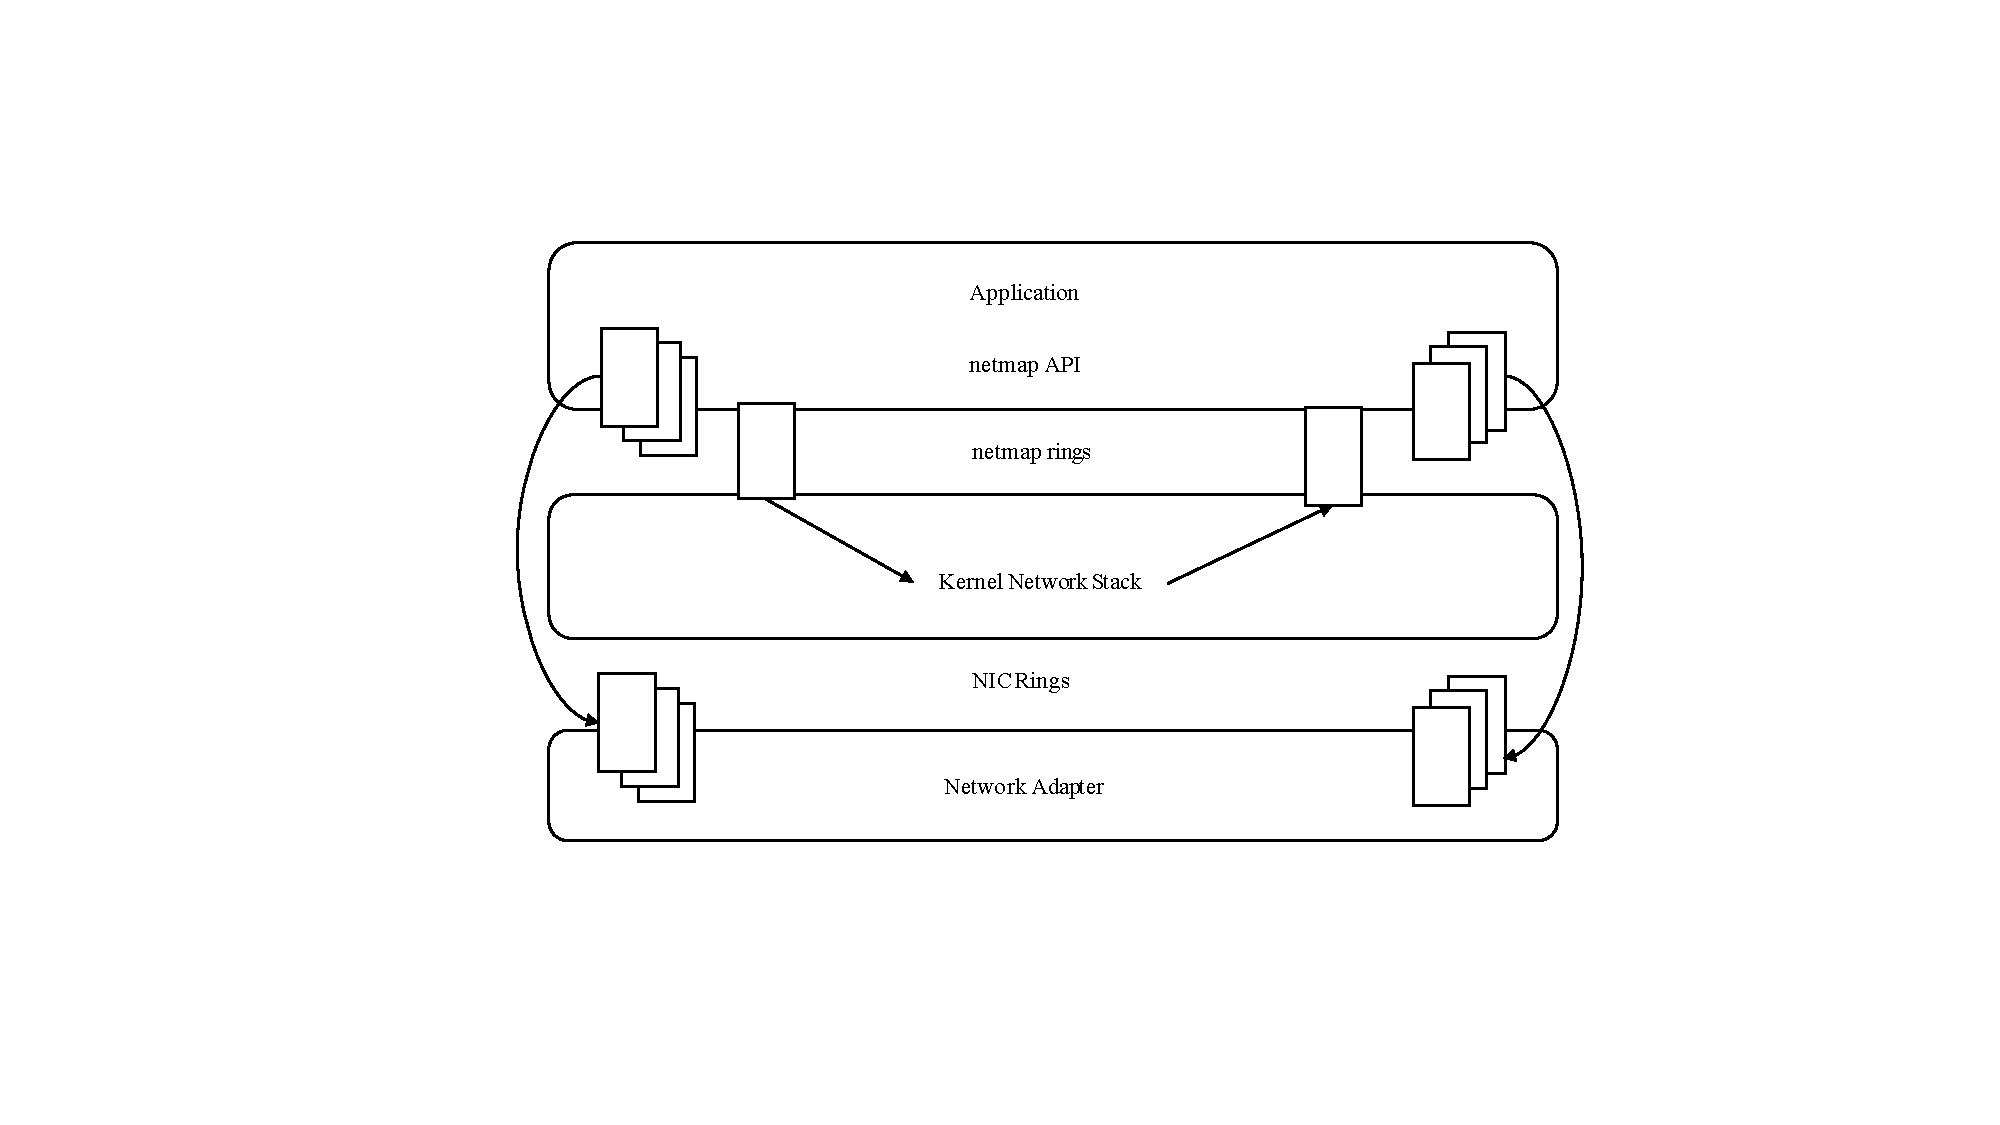
\includegraphics[width=\textwidth]{netmap}
  \caption{Netmap架构图}
  \label{fig:netmap}
\end{figure}
\vspace{-10pt}

\subsection{用户态协议栈的相关研究工作}
\label{subsec:02_userspace_related_work}

在具备高效的Kernel Bypass技术后,用户态协议栈最近几年在工业界和学术界都得到飞速发展。网络协议栈在用户态的实现可以选择两条路径,第一条是独立开发功能精简、定制化的协议栈,这样带来的网络性能提升更为可观,在定制化的场景下更具优化,然而往往缺失传统协议栈的安全性和鲁棒性;另一条路径是从传统内核协议栈中剥离出网络功能部分的代码,这需要在对熟练掌握内核协议栈实现的基础上去划分网络功能的边界,并用高速IO收发包模块的底层开发套件替换掉内核协议栈中网卡netdev、内存管理、定时器等边界函数实现,技术挑战较大,在兼顾高性能的同时可以保障系统的安全性与鲁棒性

mTCP~\cite{mTCP}是近些年学术界影响力很大并且已经开源的用户态协议栈,除了连接本地化、共享资源拆分等常见协议栈优化之外,mTCP从底层IO收包到用户态网络API都采用批处理操作,并且针对短连接进行基于优先级队列的报文处理优化策略,旨在提升短连接网络下多核系统的性能及可扩展性。其系统架构图如图~\ref{fig:mTCP}所示,底层用户态高速网络收包模块采用模块化的设计,可灵活支持PSIO、DPDK、netmap等模块,每一个CPU核拥有独立专享的TCP监听表、建连表等资源,避免锁竞争同步开销,且网络应用进程绑定在一个CPU核上,并含有一个mTCP协议栈线程执和一个网络应用线程,前者负责网络数据包的收发以及TCP/IP网络协议逻辑处理,后者负责网络应用代码执行逻辑,两者通过队列来完成线程间消息传递通信。
\vspace{-10pt}
\begin{figure}[H] % use float package if you want it here
  \centering
  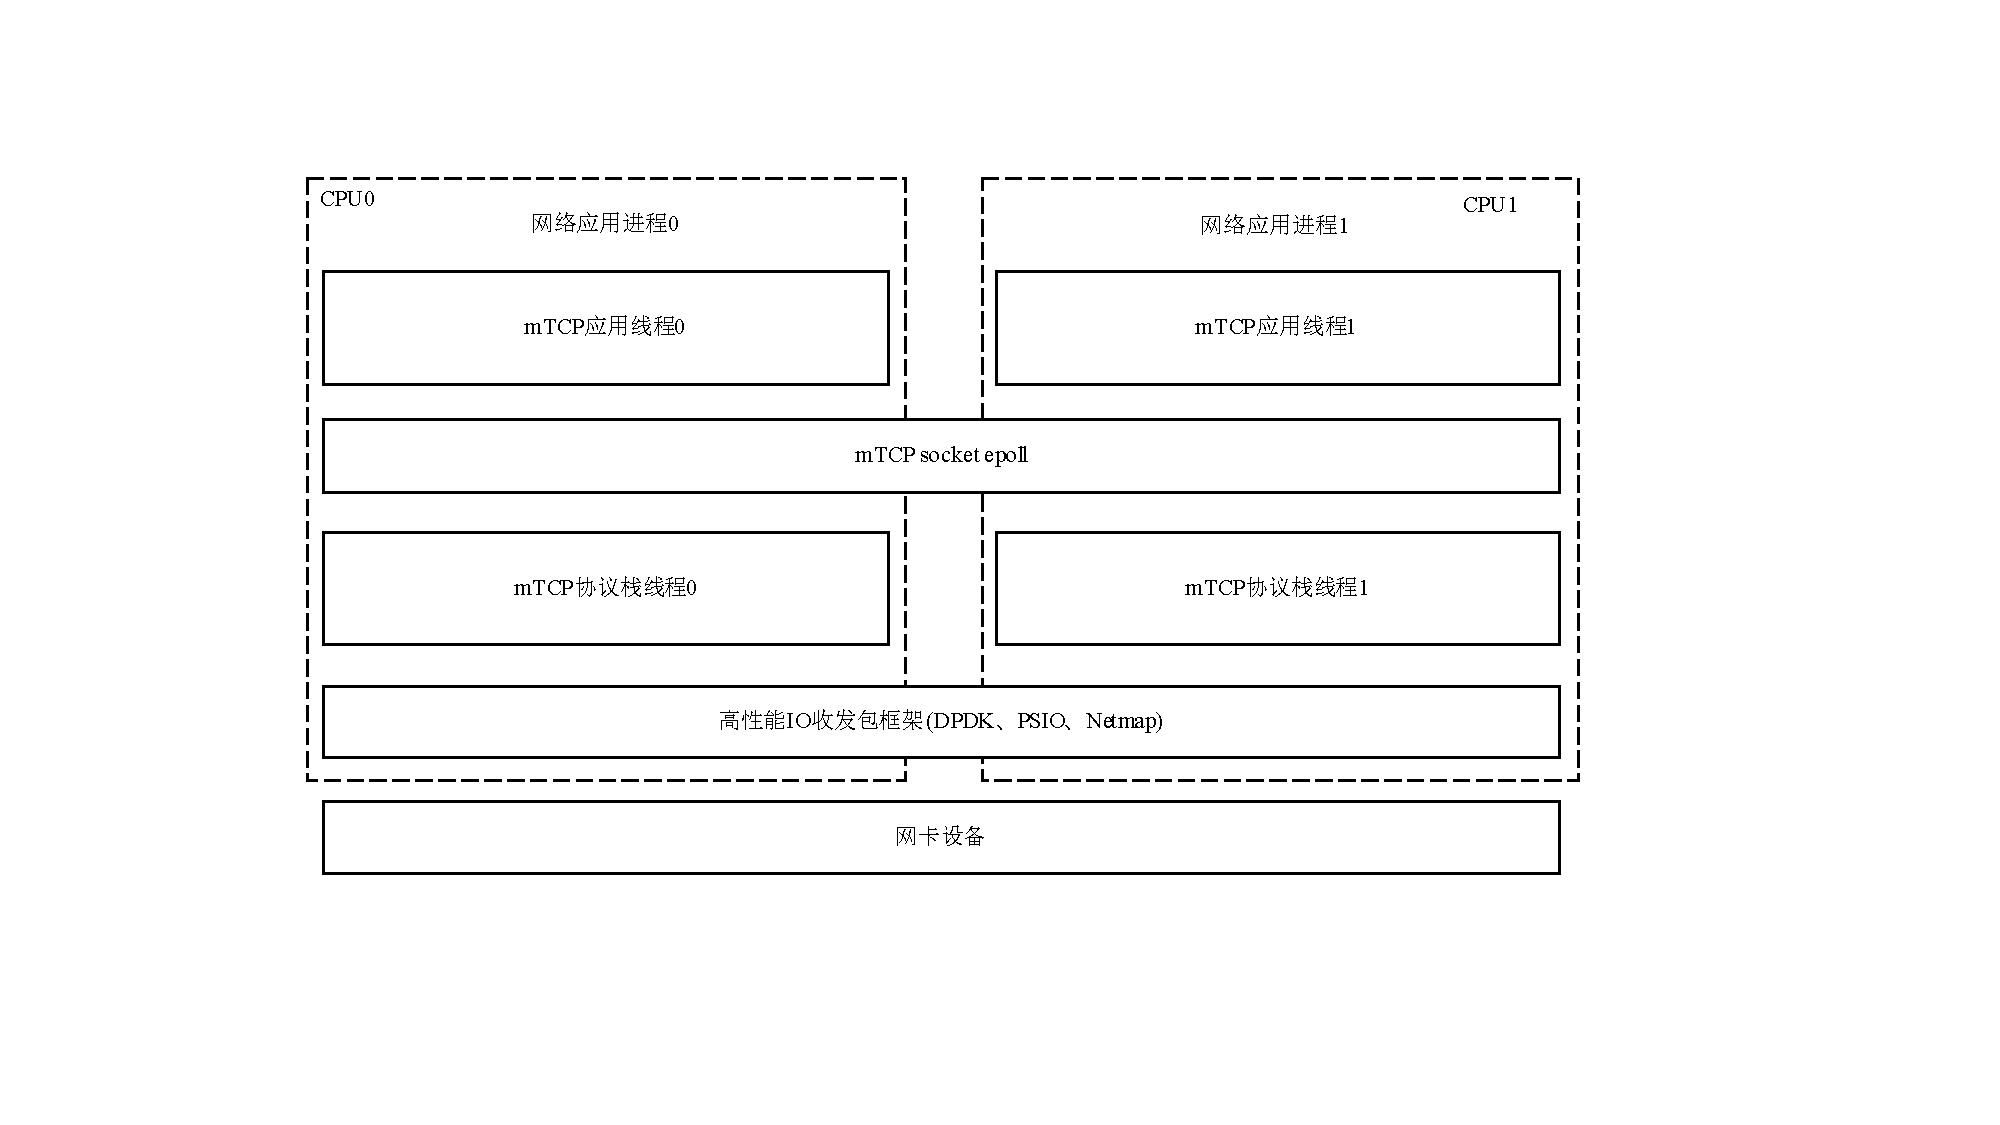
\includegraphics[width=\textwidth]{mTCP}
  \caption{mTCP架构图}
  \label{fig:mTCP}
\end{figure}
\vspace{-10pt}
不过,两个线程在同一CPU核上可能存在着严重的CPU资源争抢问题,在阅读其源码后了解到,mTCP是通过pthread条件变量来完成两个线程的调度,例如当mTCP线程完成一轮数据包的接收后产生新建连接、数据包接收等多个event,并将其放入event队列后,便会调用pthread\_cond\_signal去唤醒网络应用线程在epoll\_wait函数阻塞的执行流,而mTCP线程将会被挂起。mTCP通过这种主动让出CPU的调度策略最大程度上利用一个CPU核资源,但同时不可避免导致线程上下文切换带来的开销,mTCP是通过对接收报文、event通知的批处理操作来最大程度均摊上下文切换的开销,并且实验结果显示,mTCP在8核系统中相比于传统Linux网络协议栈带来25倍性能的提升。
然而mTCP正如其名是一个独立开发且只支持TCP传输层协议栈的网络协议栈,基于UDP的网络应用是无法应用于其上,并且其epoll接口未对非socket类型文件描述符进行支持,因为不少应用存在着用epoll对文件、管道等资源进行监控的情况,所以mTCP并不能支持这类网络应用的运行。此外,mTCP向上暴露的接口是类似POSIX API,虽然文章中指出只需要对网络应用进行少量源码修改即可,但从其开源至今四年多时间里,mTCP也仅支持了Lighttpd这个较为主流的网络应用服务器,有不少开发人员对Nginx进行移植尝试~\cite{nginxmtcp1,nginxmtcp2},但经过实验验证,均无法正常运行或者性能不及Linux内核协议栈。这也说明即使一款开源且性能优异的用户态协议栈在不具备高兼容性的情况下,其影响力也会大打折扣。

Sandstorm~\cite{Sandstorm}指出传统协议栈由于通用性带来性能瓶颈,并呼吁协议栈在数据中心这种低延迟高吞吐的网络环境下应该往专用性方向发展。然而该文章依然利用netmap作为底层IO收发包模块来减少数据拷贝,并将协议栈搬离到用户态来实现,在用户态优化协议栈的手段并未有任何创新,实验结果使用移植Nginx作为网络服务相比传统Linux内核协议栈有三倍左右的性能提升,但是其在测试SandStorm性能时将静态文件缓存到物理内存中,这与Linux内核协议栈的Nginx从磁盘中读取文件直接对比未免有失公平,这样的性能提升在兼顾通用性的用户态协议栈也能做到。所以,性能瓶颈的本质并不一定缘于协议栈的通用性或者兼容性,而是应该着眼于数据拷贝、进程间通信、系统调用、上下文切换等这些在网络协议栈中真正影响网络性能的关键。


MultiStack~\cite{Honda2014Rekindling}与StackMap~\cite{StackMap}是在用户态协议栈与兼容传统网络应用之间而采取折中策略。两者的核心思想都是将用户态协议栈与传统内核协议栈进行整合,MutiStack具体实现上最底层使用IO虚拟化技术进行Packet Demultiplex,向上承载着用户态协议栈和内核协议栈两种系统,用户态路径对应的虚拟网卡使用netmap作为收发包框架,内核态路径对应的虚拟网卡使用传统基于中断的收包模式。StackMap在设计上采用数据通道和控制通道分离的思想,数据通道通过netmap高性能收发包模块来减少数据拷贝,并向上层应用提供新型收发包API,而控制通道依然走传统内核协议栈来完成。这类折中设计只是让整个系统既可以运行传统网络应用,又能运行高性能新网络应用,不过,当下虚拟化技术非常成熟,创建一个新的虚拟机便捷又快速,这样整合的设计的意义并不大,而且其并没有解决兼容性的问题,因为网络应用若想获得用户态协议栈带来的加速依然需要根据新API语义进行重新编写。

IX~\cite{IX}采用数据平面与控制平面分离的策略,控制平面负责对CPU和内存资源配置、申请、调度和监控,数据平面负责网络协议栈的逻辑处理,并利用IO虚拟化技术将数据平面不同网络应用进行隔离,以保证安全性。IX数据平面的收包是在特定网卡上基于轮询IO模式进行的,这样可以减轻中断收包模式在大流量网络情况下由于硬件中断对CPU造成的压力。除了常见的协议栈优化策略,如图~\ref{fig:IX}展示一个IX中线程采用Run-to-Completion的工作模式,从虚拟网卡接收一个数据包,到协议栈网络逻辑处理,到交付给网络应用再到应用返回响应数据,经过协议栈后最终到达网卡进行发包,整个过程处理完才进行下一个数据包的处理,这样带来的好处是减少系统中不必要的缓存队列从而最大化降低网络延迟。当出现网络拥塞的情况,IX会对收发包和系统调用进行动态调整的批处理,以均摊上下文切换带来的开销。

\vspace{-10pt}
\begin{figure}[H] % use float package if you want it here
  \centering
  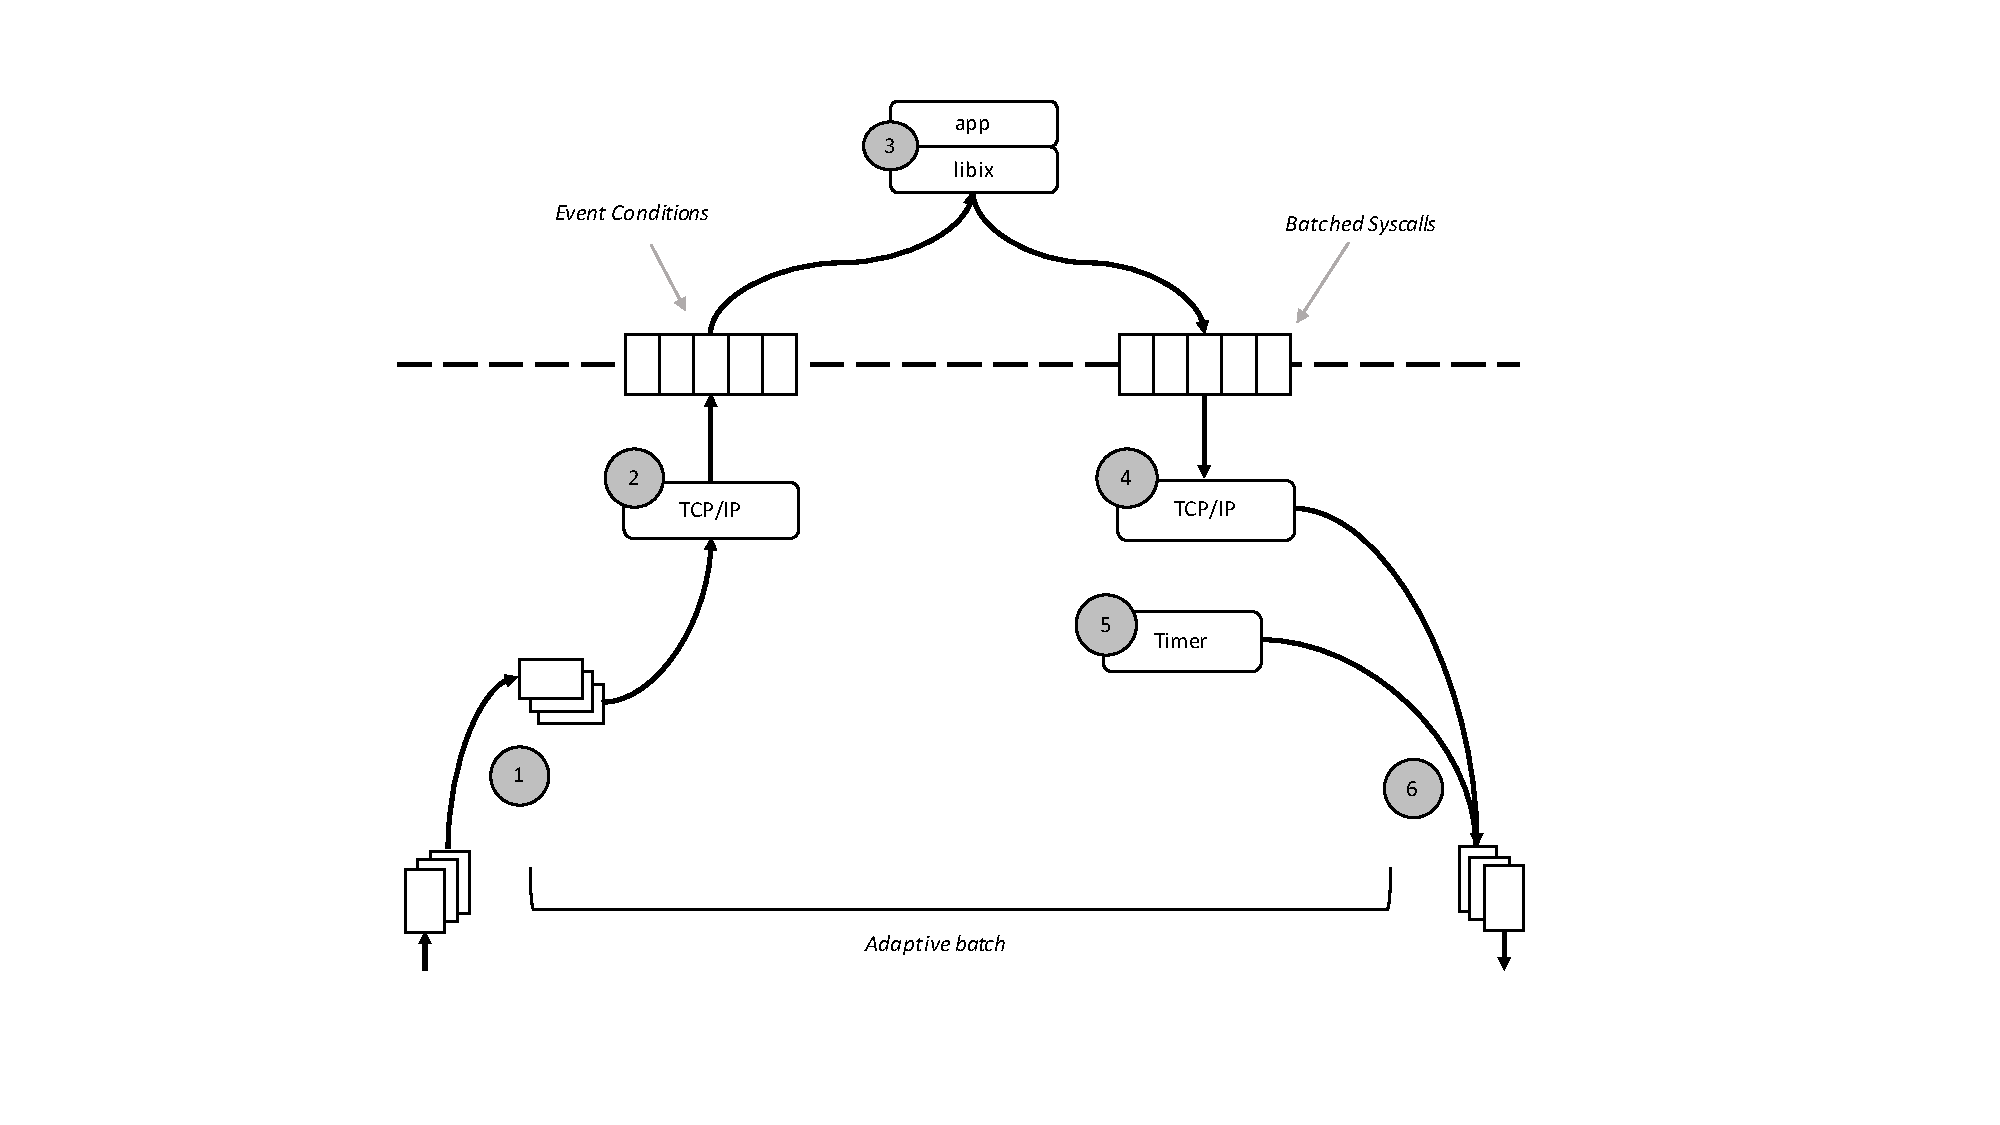
\includegraphics[width=\textwidth]{IX}
  \caption{IX Run-to-Completion工作模式}
  \label{fig:IX}
\end{figure}
\vspace{-10pt}

ZygOS~\cite{ZygOS}致力于解决网络执行流在不同核之间的调度问题而实现微秒级延迟和满足超低尾延迟要求,相比IX性能更加优秀,但两者都对网络应用毫无兼容性考虑。Arrakis~\cite{Peter2015Arrakis}也是采取将数据平面从内核中剥离的策略和IO虚拟化技术和内存映射等机制,并基于轻量级网络协议栈lwIP~\cite{lwIP}。不过该文章在兼容性方面做了更多考虑,Arrakis给网络应用暴露Native Arrakis API和POSIX API两种,前者由于重新设计数据IO的接口而实现真正的零拷贝,后者由于POSIX API 中recv 、send收发函数中带有应用buffer的语义无法实现真正的零拷贝,但也取得相比传统内核协议栈性能上的提升。

工业界近几年也开发出多款用户态协议栈~\cite{libuinet,pope2011introduction,Seastar,fstack}去加速公司网络服务性能,其中腾讯云推出的F-stack~\cite{fstack}基于DPDK高速IO收发包框架并移植FreeBSD网络协议栈来实现加速网络服务,并已经在DNS服务器、CDN接入模块等实际生产环境中落地,不过其接口是POSIX-Like,需要网络应用修改相应网络接口才能应用。Seastar~\cite{Seastar}是基于事件驱动、纯异步编程且用C++实现的用户态协议栈,其兼容性很差,因为接口是完全不同于Socket编程接口,且需要掌握更为复杂的异步编程模型。
\chapter{用户态协议栈的兼容性设计}

本章将用两节来对该用户态协议栈的设计进行详细阐述,第一节将从整体层面介绍用户态协议栈的架构,包括协议栈前后端分离的设计以及主要模块的分工、协议栈与网络应用进程间通信等。第二节从兼容性方面对协议栈的各种设计进行详细介绍,这也是该用户态协议栈最大的贡献与意义,其中包括POSIX网络系统调用接口的劫持、文件描述符空间的分割管理、Epoll IO多路复用的设计、并发流网络模型的设计、网络应用进程异常崩溃的处理机制等,通过这些设计使得该用户态协议栈在不需要修改网络应用源码的情况下就可以零成本移植,并获得网络性能的提升。

\section{协议栈整体系统设计}

用户态协议栈的兼容性的实现只有能为传统网络应用带来性能提升才会有意义,而协议栈的整体设计对整个系统的性能起到关键的作用,本节将对协议栈的整体设计进行阐述,并对其中为何这么设计的原因进行分析。
% dlsym~\cite{DLSYM}
% \cite{IO-models}
% $2^{30}$

\subsection{协议栈与应用的分核设计}

传统Linux内核网络协议栈通常是由操作系统来完成调度以及与网络应用的数据消息和控制信息的传递,而将网络协议栈搬离到用户态之后,操作系统就丧失对协议栈的绝对控制而由用户态开发人员来决定其管理与调度。用户态网络协议栈与网络应用两个执行流如何进行调度与管理成为设计之初最关键的问题,通常有两种管理方式,第一种是将协议栈执行流与网络应用执行流绑定在同一个CPU核上,比如mTCP~\cite{mTCP}就采用该种模式,此方式的优势在于减少数据跨核进行同步造成的Cache Miss,并且对CPU核资源的利用率较高,不过劣势在于协议栈执行流与网络应用执行流可能存在严重地CPU资源争抢,即使通过合理的调度机制避免CPU争夺也会存在着两种执行流在高并发高吞吐下频繁上下文切换带来的开销;第二种是将协议栈执行流与网络应用执行流分别放在两个不同的CPU核上,比如IsoStack~\cite{IsoStack}就是将协议栈处理逻辑放在专用的物理核上,该方式的好处在于可以较好地避免CPU资源的争夺,为网络协议栈收发包提供最大化的CPU资源,但其坏处是数据跨核同步带来的开销和对CPU核资源的利用率较低。本文经过实验验证,第二种方式会获得更优的网络性能,具体实验将在第五章进行详细阐述,所以该协议栈采用的是将协议栈与应用分核绑定的设计。

\vspace{-10pt}
\begin{figure}[H] % use float package if you want it here
  \centering
  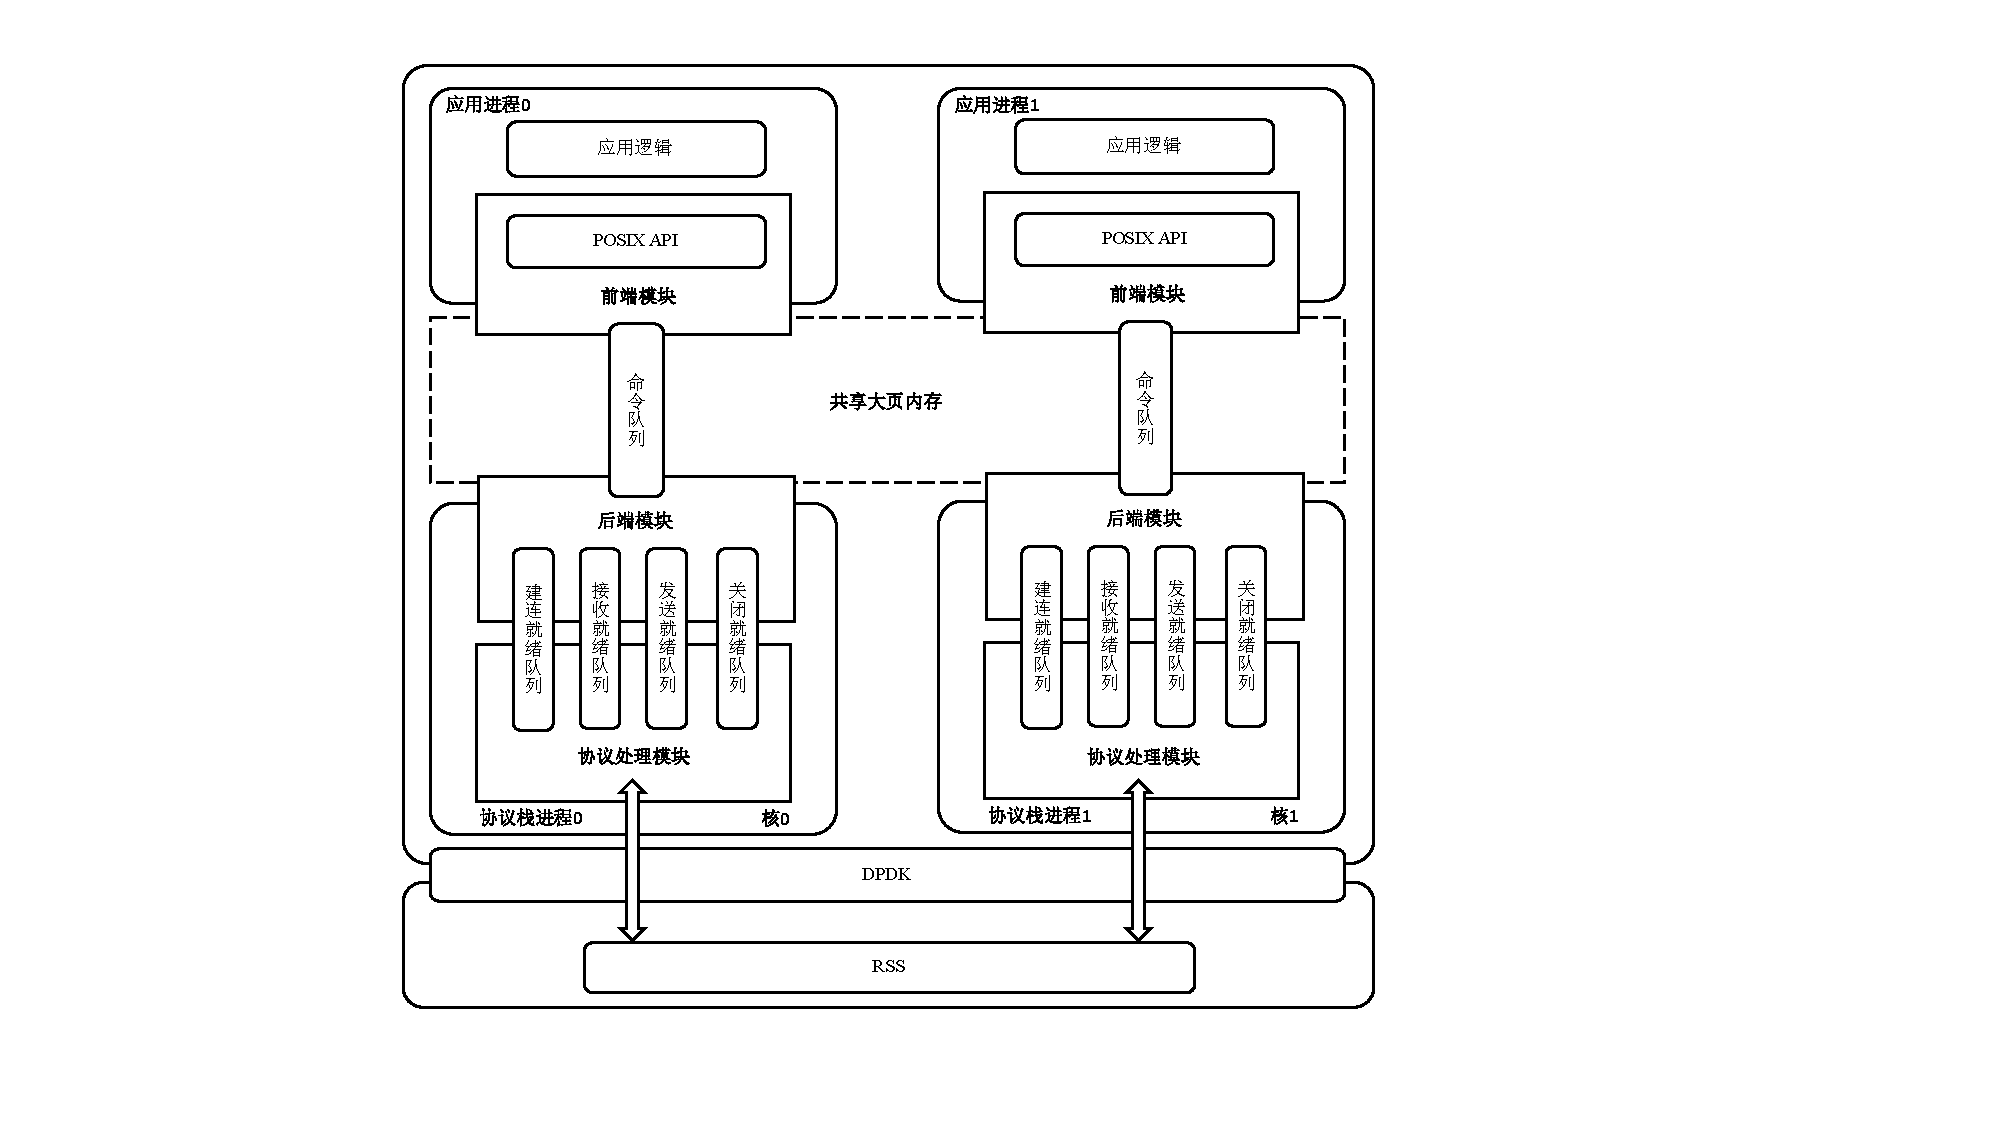
\includegraphics[width=\textwidth]{architecture}
  \caption{用户态协议栈架构图}
  \label{fig:architecture}
\end{figure}
\vspace{-10pt}

整体系统的架构图如图~\ref{fig:architecture}所示,协议栈底层使用Intel的高速IO收发包框架DPDK~\cite{DPDK},并利用RSS(Receive Side Scaling)根据接收的五元组信息和Hash算法对数据包指派到特定的CPU核上,这样该连接的所有数据包都会在该CPU核上进行处理。两个协议栈进程分别运行在两个专用的物理核上,而两者分别与对应的网络应用进程进行网络连接信息交互。网络协议栈进程由协议处理模块和后端模块组成,应用进程由前端模块和网络应用组成,前后端作为协议栈与网络应用通信的接口,基于DPDK大页内存的消息队列实现的命令队列来完成前后端通信。下面对各个主要模块进行更加详细的描述。

协议处理模块是基于Linux内核3.14.2版本中网络协议栈的代码进行剥离和二次开发,涵盖数据链路层、网络层、传输层的数据包的封装、解析、校验和状态维护。底层通过高速IO轮询收发包框架DPDK进行收发包,替代传统内核协议栈中基于中断的收包模式,减少收包硬件中断对CPU的压力。在接收方向,DPDK通过RSS技术根据对称哈希算法和五元组信息对数据包进行分配到相应的网卡队列上,接下来数据包被DPDK网卡驱动模块提供的收包函数接收到指定的协议栈进程核中,进而进入用户态数据链路层的逻辑处理以及后续的TCP状态转移,并将新建连接、读写和关闭等网络事件传送到对应的就绪队列。在发送端,DPDK根据对称哈希算法将该连接的响应报文传递到接收时的网卡队列中,从而发送给客户端。这样一个完整TCP连接的数据包的网络逻辑处理都是在同一个网卡队列、CPU核上进行处理,有利于协议栈的多核扩展性。

后端模块是整个系统大页内存、关键数据结构等各种资源的管理中心。在协议栈进程初始化时,后端init函数会对用户态套接字、文件描述符资源等资源预分配,默认socket的最大并发数是2048个,该最大并发数即可满足绝大部分的网络应用使用场景,这些申请到的套接字和文件描述符资源以资源池的形式并通过DPDK提供的无锁循环队列rte\_ring以生产者消费者模型为后续新建连接提供相应资源,并在连接断开时候将套接字和文件描述符资源进行回收,防止其发生内存泄漏。在协议栈进程初始化时还会对新建连接就绪队列、接收就绪队列、发送就绪队列、关闭就绪队列进行初始化。当协议栈完成初始化后,就进入不断地循环读取数据包、从就绪队列中读取网络事件以及处理从前端传来的网络函数调用命令,并进行相应命令的后端网络逻辑处理。当读取到新建连接或有socket新数据到来时候,就会进行FIFO写操作从而唤醒前端的内核epoll\_wait,并同时将相应的socket fd以及事件传送到前后端共享的缓冲队列中。

前端模块作为用户态协议栈最终暴露给网络应用的部分,是用户态协议栈实现高度兼容性的关键模块,其向上给应用提供与POSIX API完全一样的网络接口,这是通过LD\_PRELOAD环境变量以及动态链接技术来完成。在网络应用调用socket、read、write等函数后产生相应的命令,并放入命令队列中。此外,前端在创建Epoll结构体时,并通过内核Epoll监听额外创建的FIFO,一旦后端有事件待前端响应便进行FIFO写从而唤醒前端内核epoll\_wait调用,从而完成前端监听事件的唤醒,网络应用可以进行下一步的socket读写或新连接的建立。此外,由于用户态协议栈对POSIX网络系统调用read、epoll\_wait等进行了劫持,并且这些函数的输入参数的文件描述符可能是非网络fd,前端模块还负责对协议栈管理的网络与内核非网络文件描述符空间进行分割管理。当网络应用调用被协议栈劫持的read函数时候,如果是对socket网络文件描述符进行读操作,则走用户态协议栈的处理逻辑;而如果判定为非网络文件描述符,比如是文件系统等,则会通过dlsym~\cite{DLSYM}间接调用内核read函数来走内核流程,这样为网络应用提供完整的网络系统调用功能。前端中的兼容性设计会在下一节进行更加详细的阐述。

\subsection{进程间通信设计}
由于该系统的协议栈进程与网络应用进程是在两个不同物理CPU核上运行,传统网络服务器在高并发高吞吐的情况下会产生大量的控制消息和网络数据的传递,能否高效解决进程间通信问题就决定了能否均摊由于跨核导致的数据同步、Cache Miss等开销,对系统的整体性能尤为重要。在此,先对各种常见的进程间通信方式IPC进行简单介绍与对比,这对于为协议栈与网络应用进程间通信的抉择很有意义。

匿名管道(pipe)是操作系统早期一种进程间通信手段,数据流只能在管道中进行单向传递,只能读或着只能写,并且通信的双方只能是父子进程,这种严苛的使用条件也导致管道无法成为本系统的选择。有名管道FIFO是更高级的管道,它与pipe相比的优势在于,进程通信双方可以不具备父子关系,由于其操作起来简单方便并具备比较高的少量数据读写性能,所以FIFO被本系统用来当作后端向前端事件聚合后传递的标志位。消息队列是一种符合先入先出原则的链表,常用来实现消费者生产者模式,并且其承载的信息格式并没有限制,可以通过结构体来自由定义消息格式,所以消息队列在该系统的前后端消息传递、socket和文件描述符资源管理等多处进行使用。内核中有消息队列的实现,但是由于在频繁调用的情况下系统调用的开销也不容忽视,所以本系统基于DPDK提供的无锁消息队列rte\_ring来完成进程间消息传递的。共享内存是在进程间进行数据传递最为高效的通信方式,在物理内存中的一段地址可以通过内存映射共享到不同进程的进程地址空间,完成映射后的地址可以直接在不同进程中进行直接读写操作,本系统socket、文件描述符资源池就是基于DPDK大页共享内存提供的rte\_mempool来完成的。信号量本质上是一种多元互斥锁,当多个进程对同一个资源进行并发读写时候,往往需要信号量来进行多进程之间的同步。socket网络套接字是当前最为常用的进程间通信方式,分为远端机器之间的通信与本地的Unix域socket,后者在本系统的异常检测模块中采用。

本小节重点对协议栈与网络应用之间的进程间通信进行详细描述,网络应用在调用各种POSIX网络调用时候会将相应的指令放入命令队列中,该命令队列就是基于消息队列与共享内存来完成的,而DPDK刚好提供了一套基于CAS实现无锁化的消息队列和共享内存,即rte\_ring和rte\_mempool,两者常常需要配合使用。在协议栈初始化之时,在DPDK的primary进程中创建rte\_ring和rte\_mempool,而后DPDK的secondary进程启动之后,就通过函数rte\_ring\_lookup和rte\_mempool\_lookup来获取相应的ring和mempool的内存地址,并且这些地址都是位于DPDK统一管理的大页内存中。当应用调用POSIX网络函数后并产生一个相应命令,则从mempool资源池中获取一个真实的命令结构体地址,再将该地址enqueue进入命令队列rte\_ring中。当后端在轮询阶段,如果命令队列中有命令,就会将其dequeue之后进行该命令的相关后端操作,待完成操作之后就将该命令结构体地址返还给mempool,这样即可完成从前端向后端通信的过程。可以看出rte\_mempool类似一个资源池管理着真实的数据,而rte\_ring作为一个环形队列管理真实数据的指针。

后端在接收相应数据包或完成TCP三次握手之后需要通知阻塞在epoll\_wait的前端执行流,这就需要前端在创建epoll结构时候就为从后端到前端的信道建立一个有名管道FIFO,并且通过内核epoll完成对该有名管道的监听,当后端产生相应事件后先对该事件进行判重,防止一次同时向前端传递重复的事件,接着会将包括文件描述符、事件种类等相关信息封装后入队进事件队列,并向有名管道中写一个字节的数据,从而触发前端内核epoll\_wait返回,这样在前端再对这些网络事件并结合非网络事件统一返回给网络应用。这样就完成了从后端到前端的进程间通信过程。

\section{协议栈兼容性相关设计}

兼容性是本工作的研究重点,如何让网络应用在不修改任何源码几乎零成本地移植在用户态协议栈上需要在兼容性设计上做不少具有挑战性的工作。首先需要对网络服务器的经典模式熟练掌握,比如多进程one process per request类型,多进程主从类型,多线程one thread per request类型,Epoll IO多路复用模型以及与多进程、多线程的结合,此外还需要对Nginx、Lighttpd、Redis等主流网络应用的源码及其相关POSIX API进行充分地调研与了解,这些工作是实现对网络应用高度兼容性的前提。在这些工作的基础上就是技术上对兼容性的设计与实现,本节将从POSIX网络API的劫持、文件描述符空间的分割与管理、用户态Epoll IO多路复用机制、并发流网络模型的设计和系统异常检测机制展开进行阐述。

\subsection{POSIX网络API的劫持}

内核网络协议栈的实现有Linux、FreeBSD、Solaris等各种版本,但这些都统一遵循IEEE最初主导的POSIX(Portable Operating System Interface of UNIX)规范,该协议规定了操作系统为上层应用提供接口的标准,其中包含socket网络编程这套函数接口,这样做的好处是完全按照POSIX规范编写的应用程序可以跨Unix各种操作系统版本直接运行,所以传统网络应用基本都是遵循POSIX规范进行编写。而想要实现传统网络应用不修改任何源码的移植成本,就必须对POSIX网络API进行劫持,如图~\ref{fig:hijack}所示,让传统网络应用不调用内核操作系统的网络系统调用,即Linux的Glibc库,而去调用用户态协议栈提供的一套命名完全一样的网络接口。

\vspace{-10pt}
\begin{figure}[H] % use float package if you want it here
  \centering
  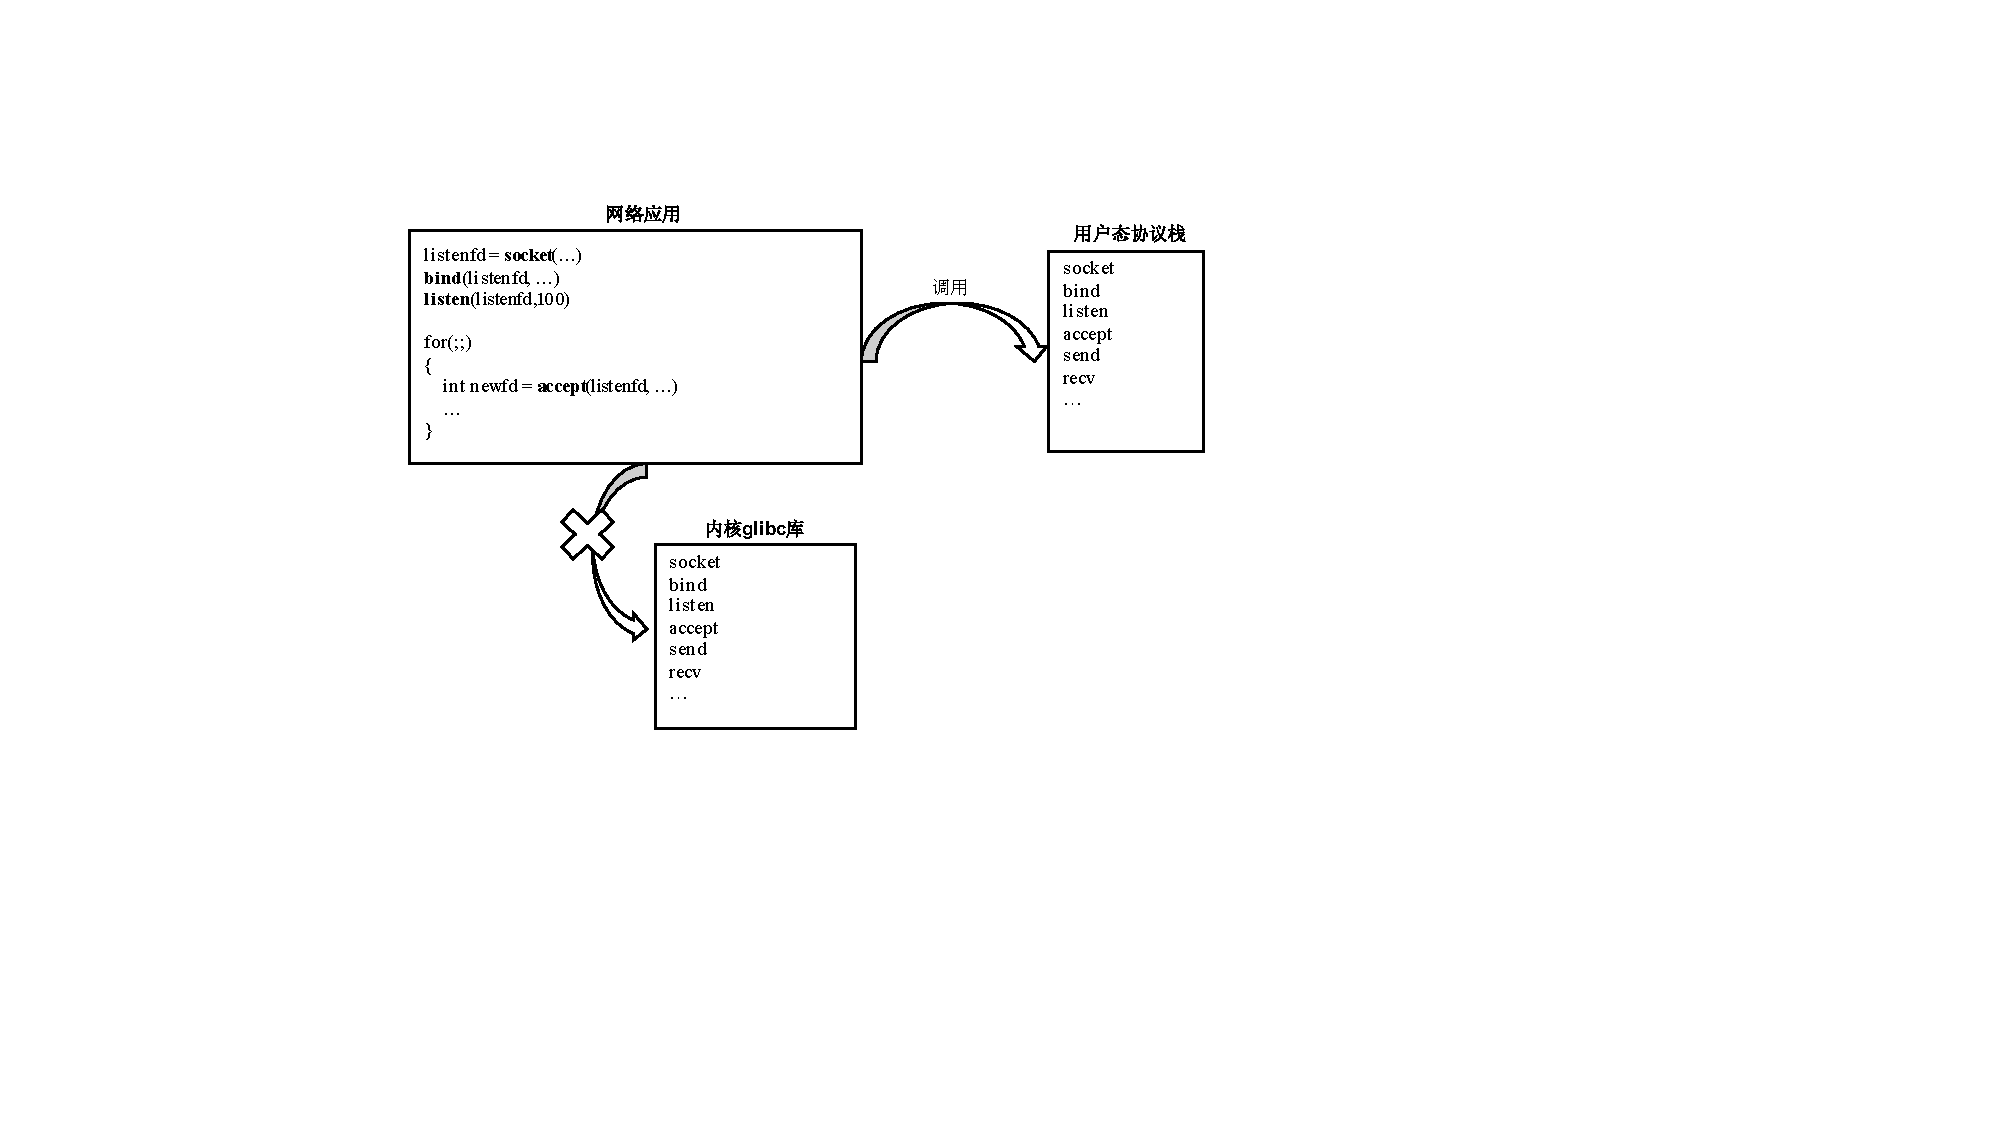
\includegraphics[width=\textwidth]{hijack}
  \caption{网络应用调用关系图}
  \label{fig:hijack}
\end{figure}
\vspace{-10pt}

本系统是在Linux环境中进行实现,而Linux中的系统调用封装成的Glibc是以动态链接库的方式被网络应用调用,动态链接相比静态链接的优势在于动态库仅需要加载到物理内存一次就可以被多个进程通过内存映射共享到其进程地址空间从而大大节约物理内存资源。本设计的劫持关键技术使用LD\_PRELOAD环境变量,它的作用是修改程序运行时加载动态链接库的优先级,尤其是当两个动态库中含有命名完全相同的函数时候。整体劫持方案如图~\ref{fig:hijack_impl}所示,首先通过userspace\_stack.c对用户态协议栈的函数重新封装成与POSIX接口完全一样,并将其用gcc编译成动态链接库stack.so。在运行网络应用可执行文件时将stack.so文件存放到环境变量LD\_PRELOAD中,这意味着stack.so动态库的加载优先级高于POSIX系统调用动态库libc.so。当传统网络应用在运行到调用网络API时,首先会先加载Linux系统中的ld.so动态连接器,它是进程加载其他链接库的桥梁,接下来会直接调用stack.so动态库中socket函数的实现;而当传统网络应用调用非网络API时,依然会调用libc.so中的内核系统调用。但是read、epoll\_wait等相关API的实现依然需要借助内核read、epoll\_wait来实现阻塞或磁盘文件IO等操作,所以stack.so又通过dlsym运行时动态链接技术对内核进行间接调用,并将其命名为kernel\_xxx以便区分,这会在文件描述符空间管理和Epoll多路复用设计小节中详细描述。

LD\_PRELOAD来实现网络系统调用的劫持几乎没有性能损耗,并且该方案对apache网络服务器通过其他网络库间接调用glibc动态库的模式依然有效,当然这种方式目前只能对调用POSIX API且C语言实现的传统网络应用有效,至于最新基于golang等语言的网络服务并不在本工作的考虑范围之内。

\vspace{-10pt}
\begin{figure}[H] % use float package if you want it here
  \centering
  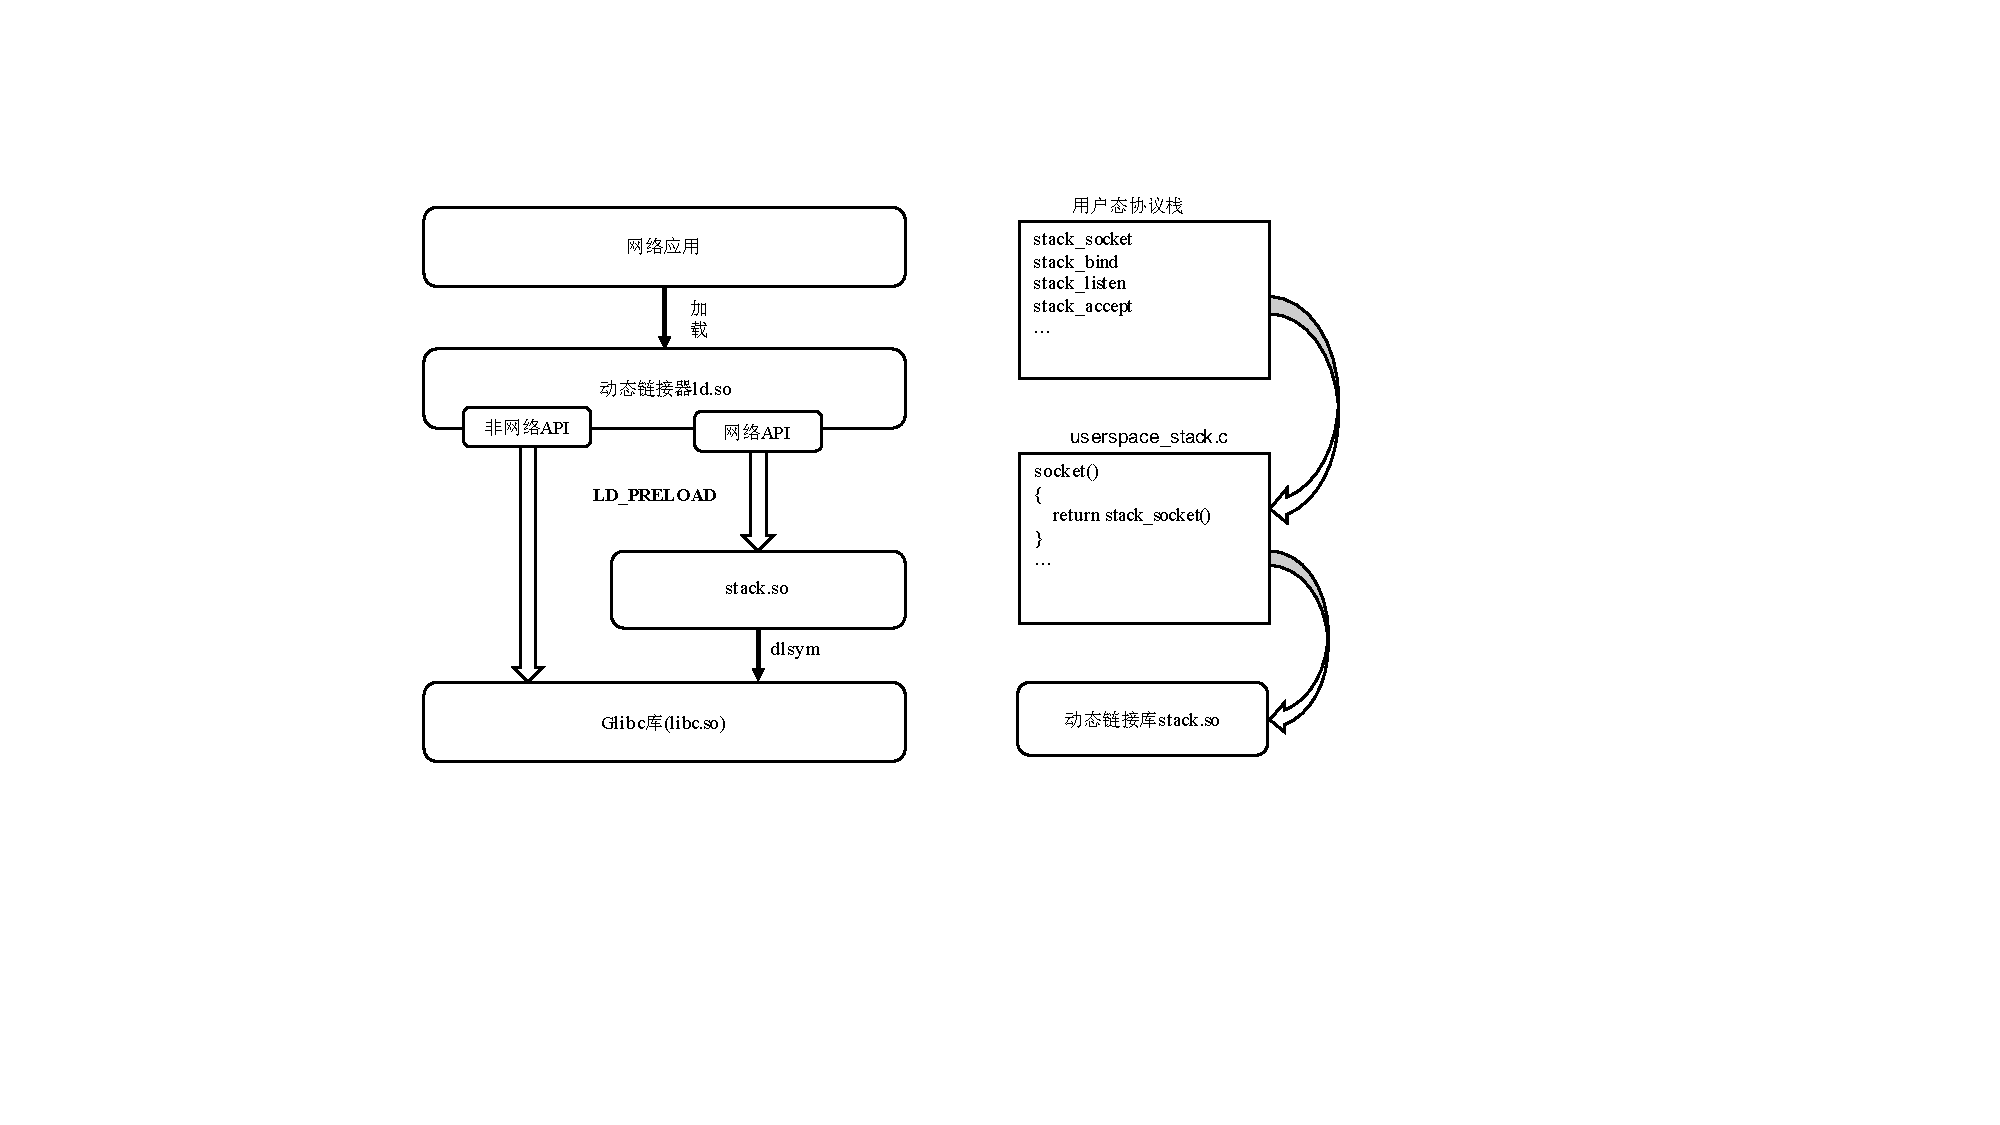
\includegraphics[width=\textwidth]{hijack_impl}
  \caption{劫持POSIX网络API设计图}
  \label{fig:hijack_impl}
\end{figure}
\vspace{-10pt}

\subsection{文件描述符FD空间的管理}

劫持POSIX网络相关API引入一个新的问题,那就是read、epoll\_wait等函数参数中的文件描述符可能并不只是socket网络文件描述符,比如读写一个磁盘文件或epoll监听一个有名管道等,而用户态协议栈仅仅实现了操作系统中TCP/IP协议栈,并不对非网络功能进行支持。所以在传统应用调用被用户态协议栈劫持的read等函数之后,就需要先对文件描述符进行分割管理,socket网络文件描述符调用用户态协议栈处理逻辑,而非网络文件描述符依然调用内核kernel\_read函数,这也是stack.so文件依然需要使用dlsym对内核系统调用进行链接的原因。

由于文件描述符是有符号型整数,最简单的实现方案就是将文件描述符整数空间一分为二,如图~\ref{fig:split_fd1}所示,以$2^{30}$作为分界点,从左向右为非网络文件描述符FD,并调用内核系统调用。而如果是socket网络文件描述符则根据$2^{31}-1 - fd$重映射到右边大整数的空间。这样传入的文件描述符如果不小于$2^{30}$则为socket网络文件描述符,并走用户态协议栈逻辑,而如果小于$2^{30}$则为非网络并进行内核系统调用。由于在实际百万级高网络并发的条件下,socket连接数也远小于$2^{30}$,所以该方案理论上是可行的,并且本文初期就采用该方案成功移植Nginx网络应用。然而在Lighttpd、Redis等网络应用中常常需要将socket文件描述符作为数组下标,该方案返回的socket文件描述符过大必然会造成数组越界访问,从而引发系统崩溃。

\vspace{-10pt}
\begin{figure}[H] % use float package if you want it here
  \centering
  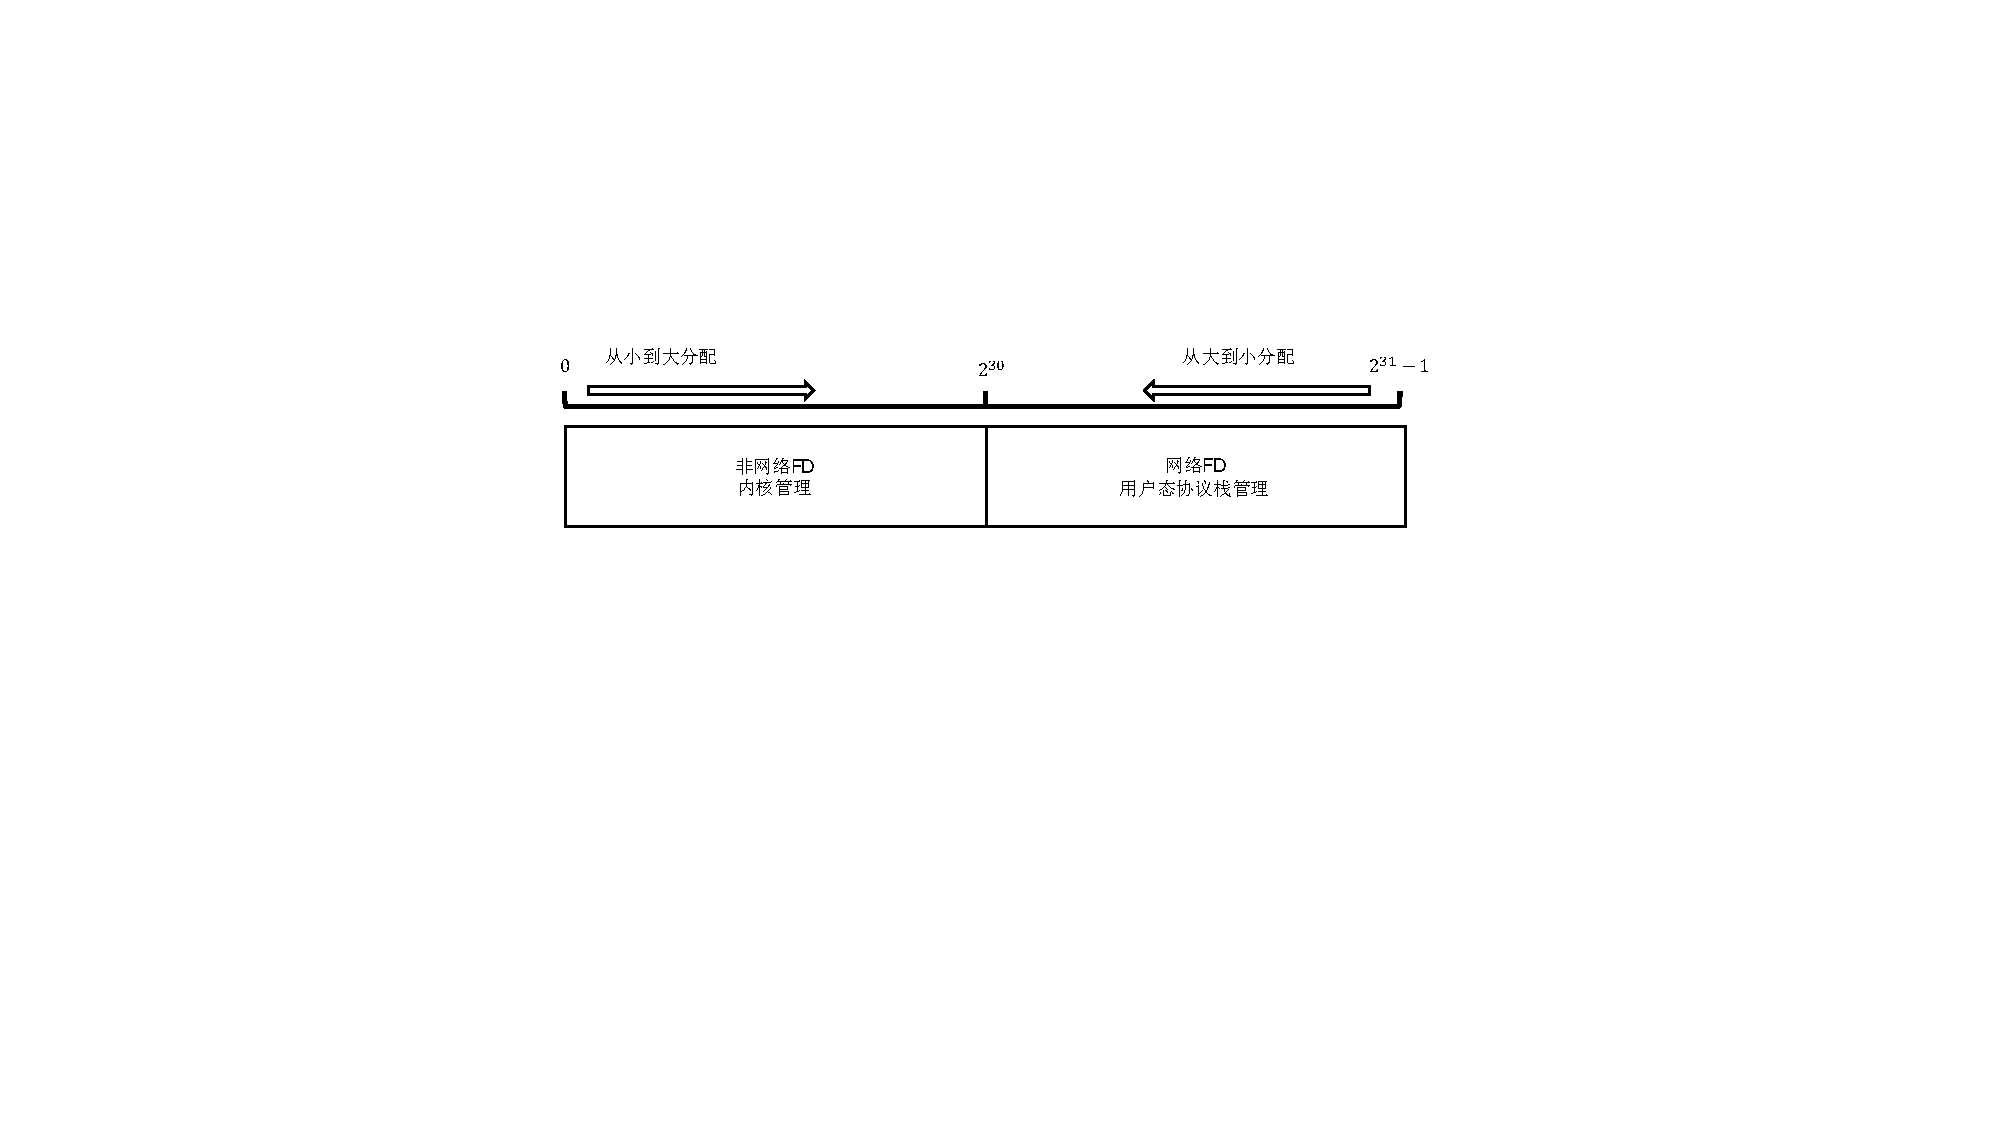
\includegraphics[width=\textwidth]{split_fd1}
  \caption{文件描述符空间管理方案一}
  \label{fig:split_fd1}
\end{figure}
\vspace{-10pt}

为了解决socket文件描述符过大的问题,本文基于资源预分配和双向映射设计了第二种更为科学的文件描述符管理方案。如图~\ref{fig:split_fd2}所示,当用户态协议栈在初始化时会调用多次kernel\_socket函数去申请傀儡文件描述符并放入fd资源池中,这样这些fd号就提前被该网络应用进程占用,与此同时也会对socket资源提前进行预分配并放入对应的资源池中。当网络应用调用socket或者accept产生一个新连接时,就分别从fd资源池和socket资源池中获取相应的真实fd和协议栈socket数组下标,并建立两者的双向映射关系,方便互相索引查找。当该socket连接关闭的时候,再将真实fd和socket协议栈资源回收,并将双向映射关系重置。这样返回给网络应用的socket fd就是比较小的整数,解决了数组越界访问的问题。
\vspace{-10pt}
\begin{figure}[H] % use float package if you want it here
  \centering
  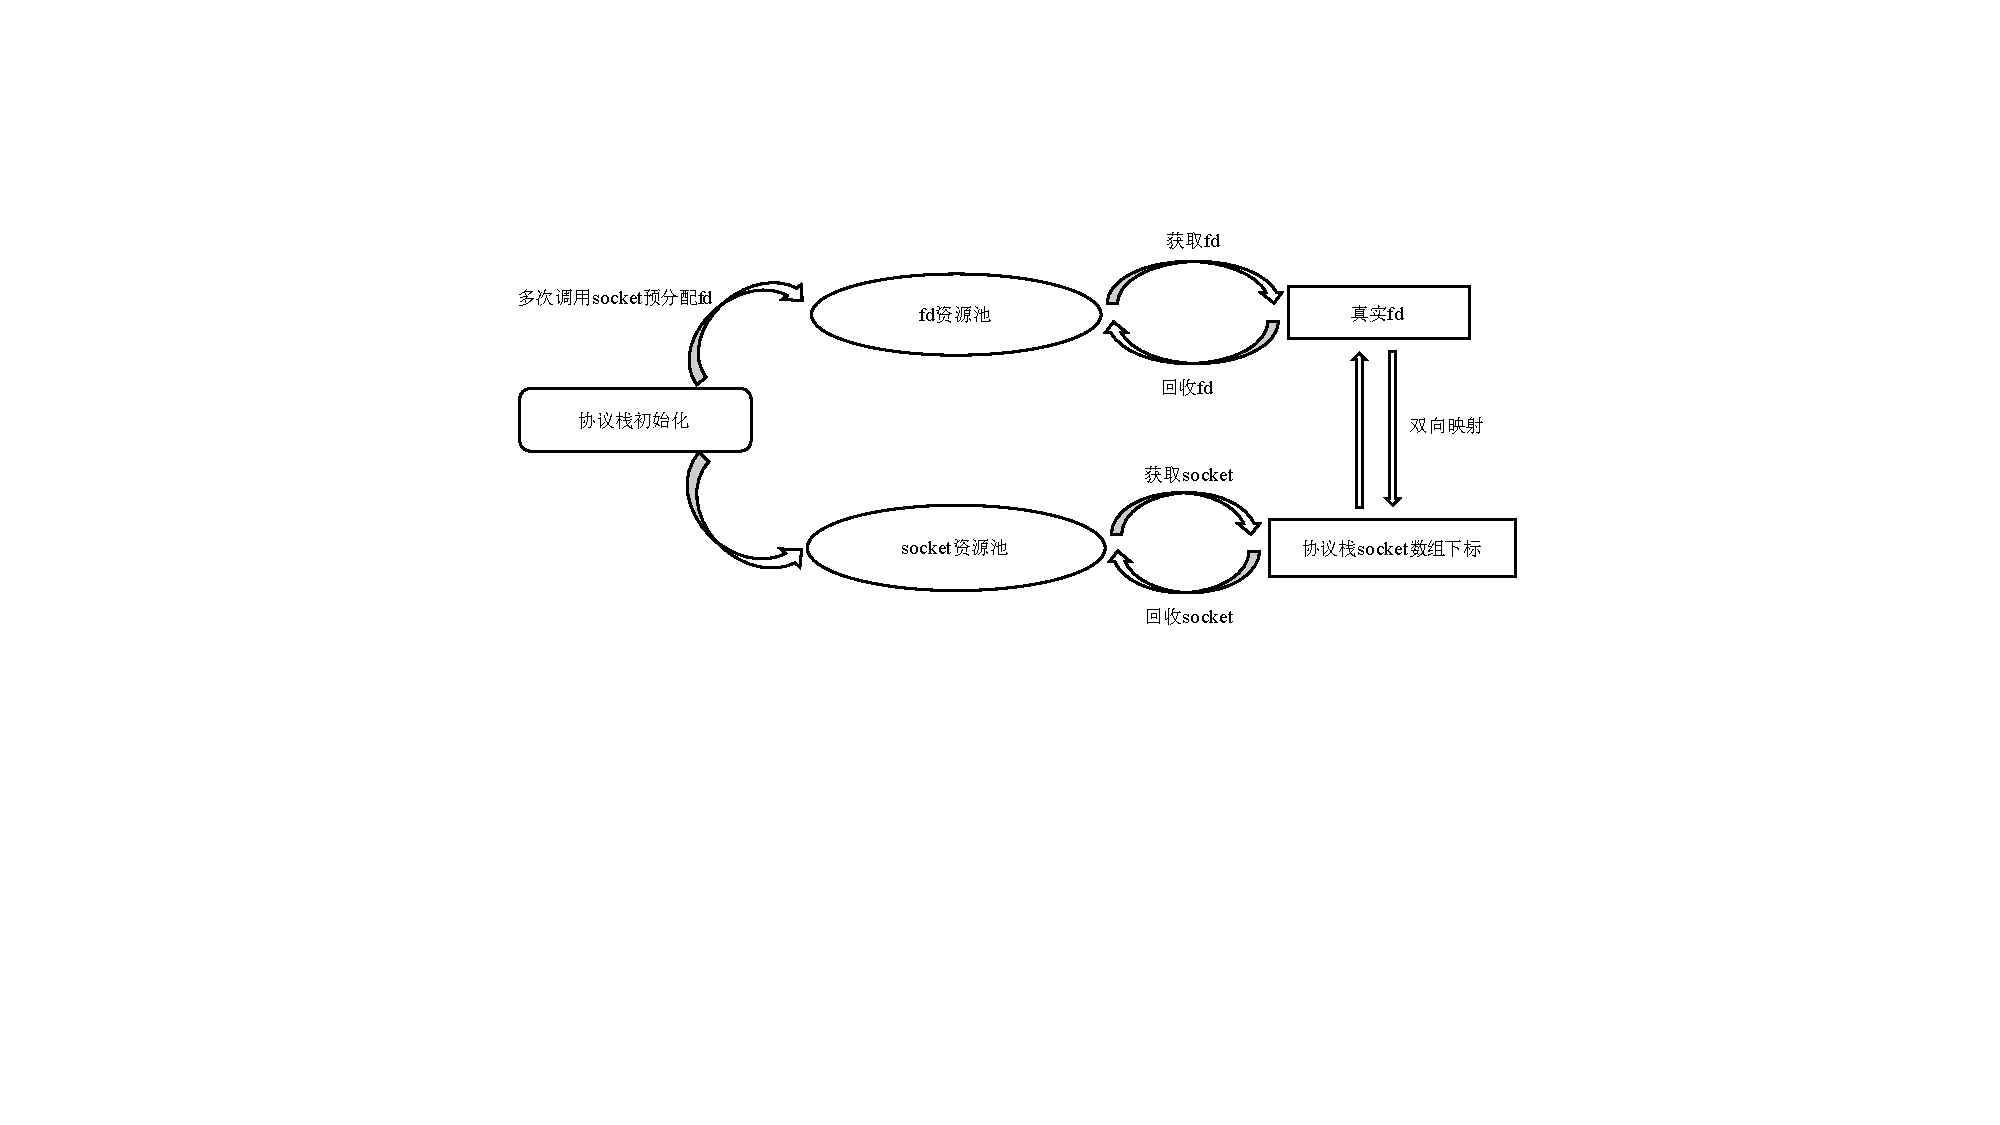
\includegraphics[width=\textwidth]{split_fd2}
  \caption{文件描述符空间管理方案二}
  \label{fig:split_fd2}
\end{figure}
\vspace{-10pt}

此外,资源预分配也降低了新建网络连接时候资源分配的成本以及性能损耗,不过由于预分配的资源有限,一旦网络并发数过大超过资源上限,就必须再分配足够的资源重新放入资源池,否则将出现新建连接失败的情况。所以本系统也为fd和socket资源池设计动态伸缩方案,当资源池剩余资源个数低于总资源数量的10\%将通过Unix域socket通知异常检测模块,并再分配足够的资源放入资源池当中。当资源池中剩余资源个数高于总数的90\%、资源池总数高于初始值且维持该状态超过两分钟之后,也通过异常检测模块,将一部分资源进行回收,选取两分钟的时间是因为HTTP长连接的时间大多1分钟左右。资源池的动态伸缩也将在系统异常检测机制一节进行更加详尽地阐述。

\subsection{Epoll IO多路复用的设计}

IO多路复用技术可以让高并发网络连接可以在一个执行流中实现,Linux系统中常见的IO多路复用技术包括poll、select、epoll。前两者的效率较低并且支持的并发连接数受限,而epoll的出现在一定程度上解决传统网络中的C10K问题,这主要得意于epoll在内核中利用在高速缓冲区建立的红黑树和就绪链表数据结构分别表示监听事件和已就绪事件,每次返回给网络应用都是已就绪事件集合,大大降低网络高并发时候的开销。也正是因为epoll的效率之高,所以在传统网络应用Nginx、Lighttpd、Redis中等被广泛应用。在用户态实现高效的epoll事件监听通知机制就成为该用户态协议栈兼容这些主流网络应用的关键。

在数据结构设计上,用户态协议栈的epoll借鉴内核epoll的设计,采用了红黑树这种高效的平衡二叉搜索树,其可以在$log(n)$时间复杂度内完成结点的插入、查找和删除操作,这在网络并发很高时候作用较大。不过,当网络并发较小的时候,红黑树这种较为复杂的数据结构性能反而不高,所以设计上采用双向链表和红黑树结合的数据结构来表示某个epoll结构体监听事件集合,当网络并发较小的时候采用双向链表,当并发数增加之后就将双向链表转换成红黑树从而加速高并发时的操作。

在完成数据结构方面的设计之后,用户态协议栈的epoll依然有两个关键技术难点需要解决。第一个难点是如何对socket网络事件和非网络事件同时实现监听与响应,第二个难点是在用户态如何判断有事件已经就绪并返还给网络应用。在用户态由于控制权限较低无法直接对进程的状态进行调度,最简单的思路就是另起一个线程对就绪事件进行不断轮询,一旦轮询到有事件待相应就返回给网络应用,但这种方式对CPU资源的消耗过大。而本协议栈主要通过有名管道和内核epoll解决如上的问题,具体用户态epoll整体架构图如图~\ref{fig:epoll}所示,整个用户态epoll流程分为以下几个步骤:

\begin{enumerate}[(1),labelsep=.5em, leftmargin = 0pt, itemindent = 3em]
\item 当网络应用调用用户态epoll\_create时,前端从epoll资源池中获取一个用户态epoll结构体,并对其进行初始化。初始化过程包括对用户态epoll的双向链接监听结构体进行初始化以及通过kernel\_epoll\_create创建一个内核epoll结构体和有名管道FIFO,并用内核epoll对该FIFO进行监听,为后续事件相应唤醒作准备。最后返回给网络应用一个预分配的epoll fd。
\item 当网络应用调用用户态epoll\_ctl时前端会对被监听文件描述符进行判断,如果是非网络文件描述符,则调用内核epoll\_ctl用内核epoll来操作该事件;而如果是网络文件描述符,添加事件操作则将该事件添加到用户态epoll的双向链表结构体中,并在事件数量超过某一阈值后将双向链表转换成红黑树,其他修改、删除操作也是类似。

\vspace{-10pt}
\begin{figure}[H] % use float package if you want it here
  \centering
  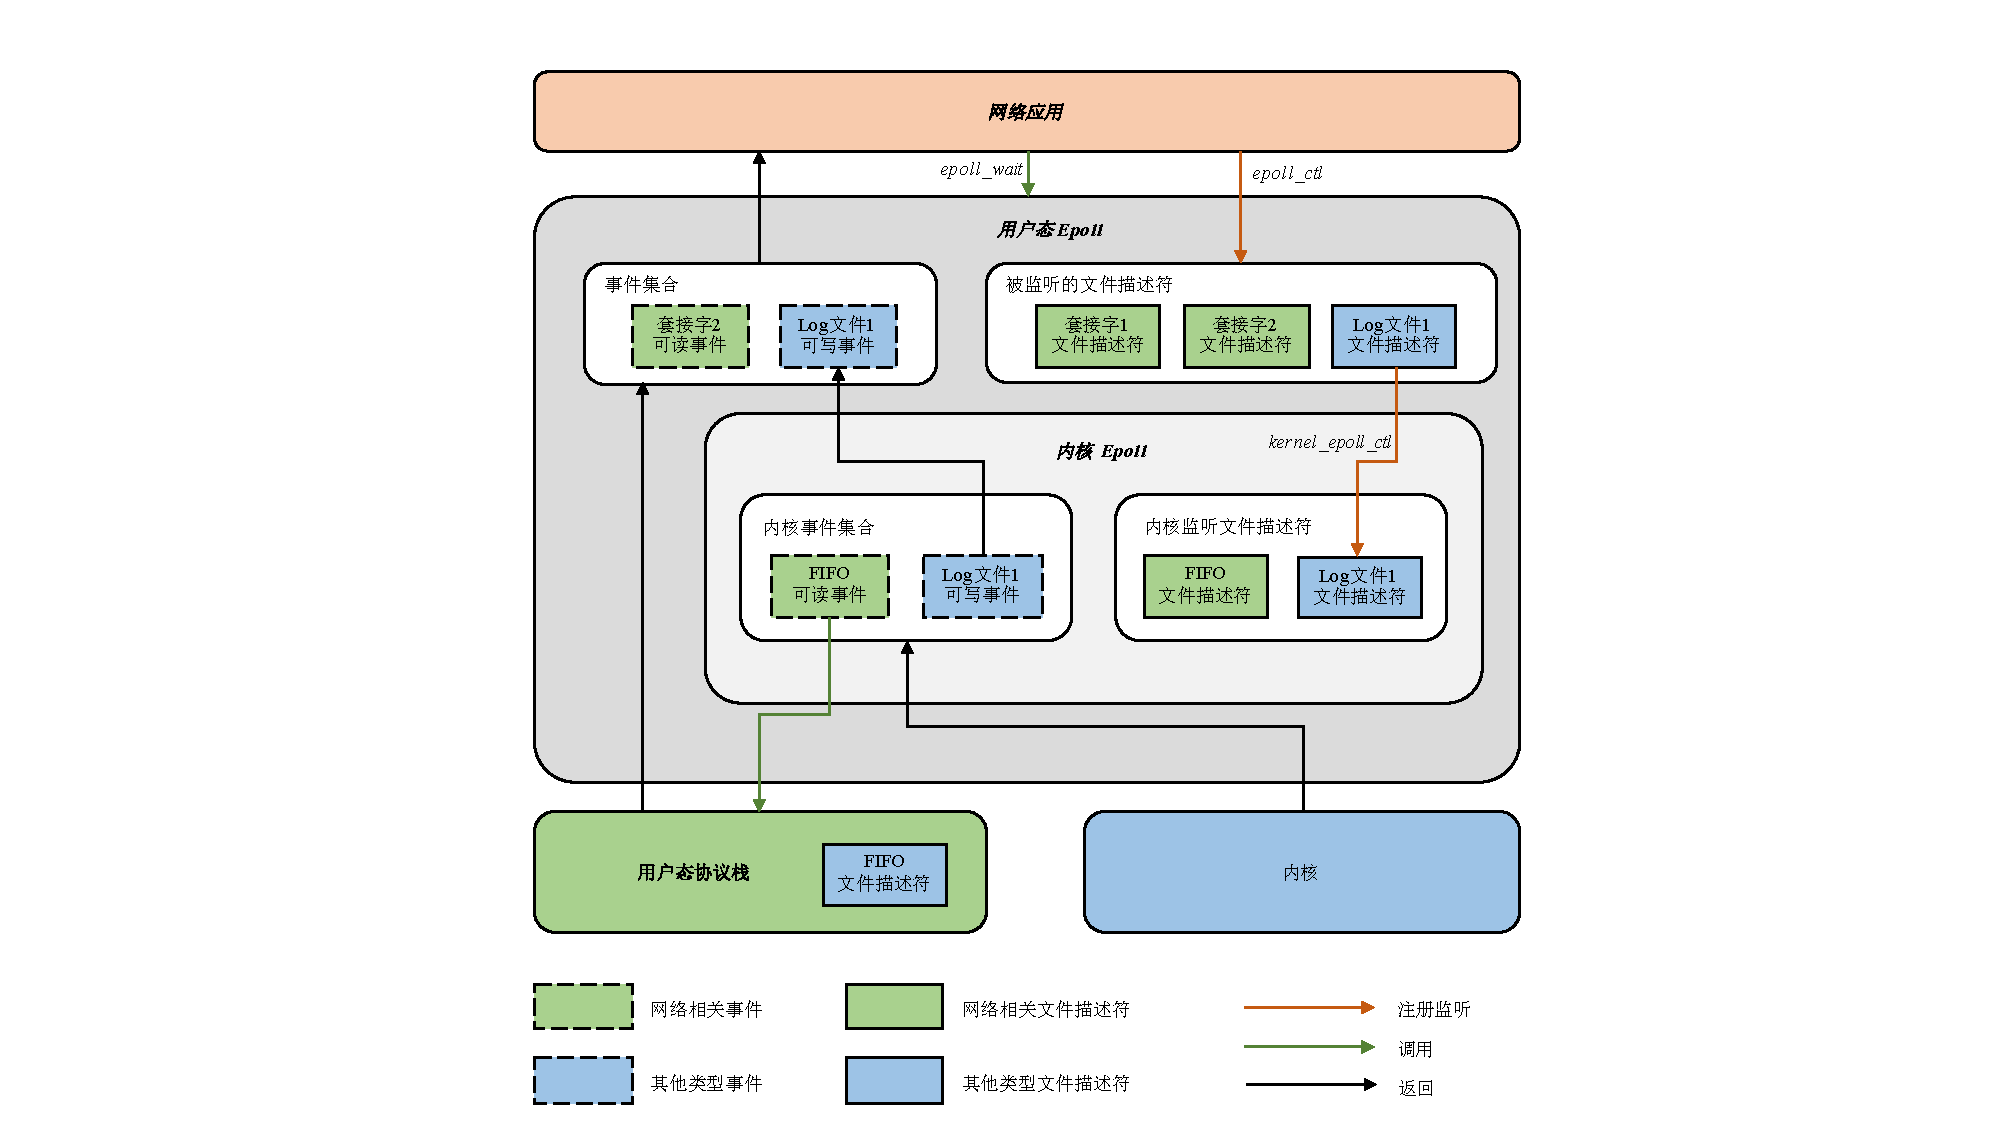
\includegraphics[width=\textwidth]{epoll}
  \caption{用户态epoll设计图}
  \label{fig:epoll}
\end{figure}
\vspace{-10pt}

\item 当网络应用调用用户态epoll\_wait时,会根据timeout参数判断该调用是阻塞还是非阻塞的,如果timeout为0则直接从用户态epoll就绪事件消息队列中获取事件并返回给网络应用,如果timeout大于0则会调用内核epoll\_wait进入休眠阻塞,此时内核epoll同时监听FIFO和应用注册的非网络事件。
\item 当后端接收到新建连接的、socket的可读可写等事件之后,将这些事件进行聚合批量地传递到用户态epoll的就绪事件消息队列中,并向其FIFO写一个字节数据,这样对应的kernel\_epoll\_wait就会被唤醒。此外,非网络事件通过内核渠道的事件触发以及timeout时间到达均可唤醒kernel\_epoll\_wait。
\item 当kernel\_epoll\_wait被事件唤醒之后,便将对应FIFO中的数据全部读出来,并对网络就绪事件消息队列进行全部出队操作,并与内核epoll监听的非网络事件进行聚合,于是网络事件和非网络事件就统一起来返回给网络应用,并等待着下一轮的用户态epoll\_wait调用。
\end{enumerate}

通过以上的设计,用户态epoll就解决了同时对网络文件描述符与非网络文件描述符的监听事件问题,并能在尽可能少占用CPU资源的前提下及时唤醒用户态epoll\_wait并返回给网络应用待响应的事件。

\subsection{并发流网络模型的设计}

在IO多路复用之前,网络服务器在accept出一个新连接后需要创建一个新进程或者线程来对新连接进行读写处理,在连接关闭之后进程或线程就退出,进程或线程不断的产生与销毁对于服务器性能产生过多的损耗。于是在内核网络协议栈陆续推出了poll、select、epoll,其中epoll由于高效的网络并发处理能力而被广泛应用于当下的网络服务器中。然而随着CPU硬件向多核架构方向不断发展,并发执行流结合IO多路复用开始成为当前多种主流网络服务器采用的网络模型。比如Nginx网络服务器可配置成多进程工作模式,如图~\ref{fig:nginx_multiprocess}所示,master进程在完成listen socket的创建之后调用fork产生多个worker进程,多个子进程worker同时监听一个listen socket,并由worker子进程循环调用epoll\_wait监听事件进行网络处理,整个网络服务器master仅负责对worker子进程的监控与管理,而所有网络连接请求的处理由worker进程来完成。Lighttpd也有着与Nginx几乎一样的多进程模式,而像是memcached则是IO多路复用与多线程结合的网络模型。本用户态网络协议栈由于采用协议栈进程与网络应用进程分核的设计,并且协议栈底层使用DPDK轮询IO模式收包占用较多的CPU资源,所以合理对网络应用并发流进行CPU资源和协议栈资源的调度减少或尽量避免CPU资源的争抢是并发流网络模型设计的关键。

\vspace{-10pt}
\begin{figure}[H] % use float package if you want it here
  \centering
  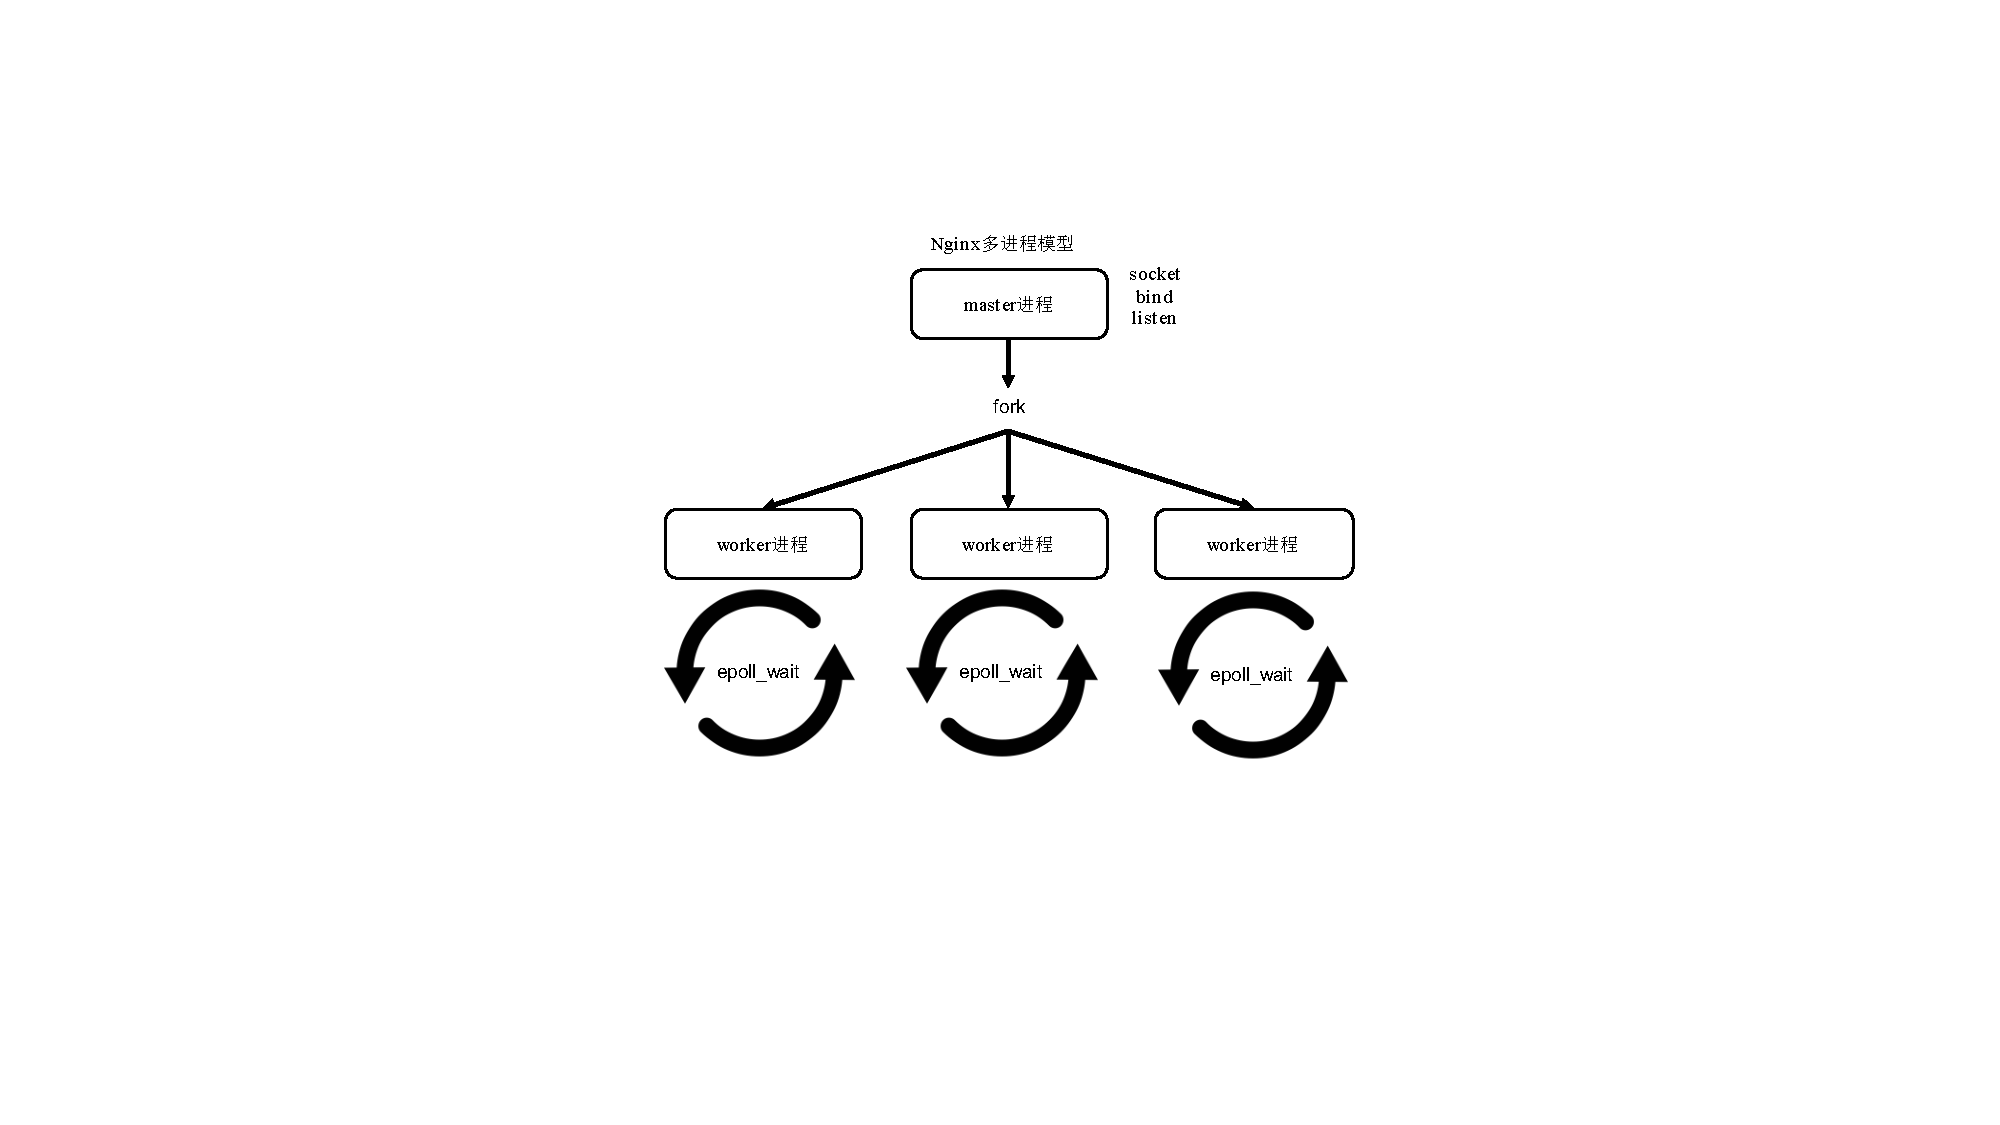
\includegraphics[width=\textwidth]{nginx_multiprocess}
  \caption{Nginx多worker工作模型}
  \label{fig:nginx_multiprocess}
\end{figure}
\vspace{-10pt}

本工作利用DPDK的亲核性通过修改启动脚本将多个协议栈进程分别绑定在专用的CPU核资源上,作为网络事件的生产者进行网络数据包的接收与发送以及网络协议的处理。而对于网络应用执行流(包括进程或线程),则需要为每个执行流分配合适的CPU核与为其提供网络服务的协议栈进程,所以将CPU与提供网络服务的协议栈进程抽象为资源池,CPU资源池可以根据用户配置来决定系统中哪些可用的CPU核作为运行网络服务执行流的资源,而默认配置则将除了协议栈进程占用的CPU核均作为资源池,资源池中资源的获取依据最少服务原则。

对于多进程worker网络模型,当应用调用被劫持的fork函数产生子进程后,依据最少服务原则从CPU资源池中选取其中一个进行亲核性设置,即运行网络应用执行流个数最少的那个CPU会被选定,协议栈进程也根据同样的原理进行选定,并将该子进程worker与选取后的协议栈进行绑定,组成一个协议栈与worker进程对,即该应用进程所有的网络连接最后都在指定的协议栈进程进行处理。由于子进程的地址空间与父进程根据Copy on Write原则相互独立的,并且网络应用中经常出现子进程中关闭父进程中的socket fd的情况,所以本系统也为用户态协议栈引入了与内核类似的socket引用计数机制,即fork之后父进程的用户态socket的引用计数自增,在子进程调用用户态close之后只将用户态协议栈管理的引用计数减1,只有当其引用计数减为0之后才运行真正关闭用户态socket并回收相关资源的操作。对于多线程网络模型的支持,整体与多进程模型相似,主要也是根据最少服务原则为该线程选取CPU核以及协议栈进程,但线程之间不存在文件描述符资源共享的问题,所以也不需要在线程新创建与退出时操作用户态socket的应用计数。除此之外,网络应用进程或线程异常退出时也要将socket和文件描述符资源返还给资源池,防止资源内存泄漏,具体实现会在系统异常检测设计一小节进行详细阐述。

\subsection{系统异常检测设计}

网络服务器应用常作为后台守护进程驻留在系统中一直运行,所以必须防止可能发生的内存泄漏从而避免应用消耗大量宝贵的物理内存资源。这就需要专门的异常检测模块来对网络应用进程进行监控,一旦发生异常崩溃退出后可回收其套接字和文件描述符资源。一些主流网络服务器比如Nginx会对worker异常退出进行监控并重启创建新的worker,但用户态套接字等资源还需要由用户态协议栈来管理。

\vspace{-10pt}
\begin{figure}[H] % use float package if you want it here
  \centering
  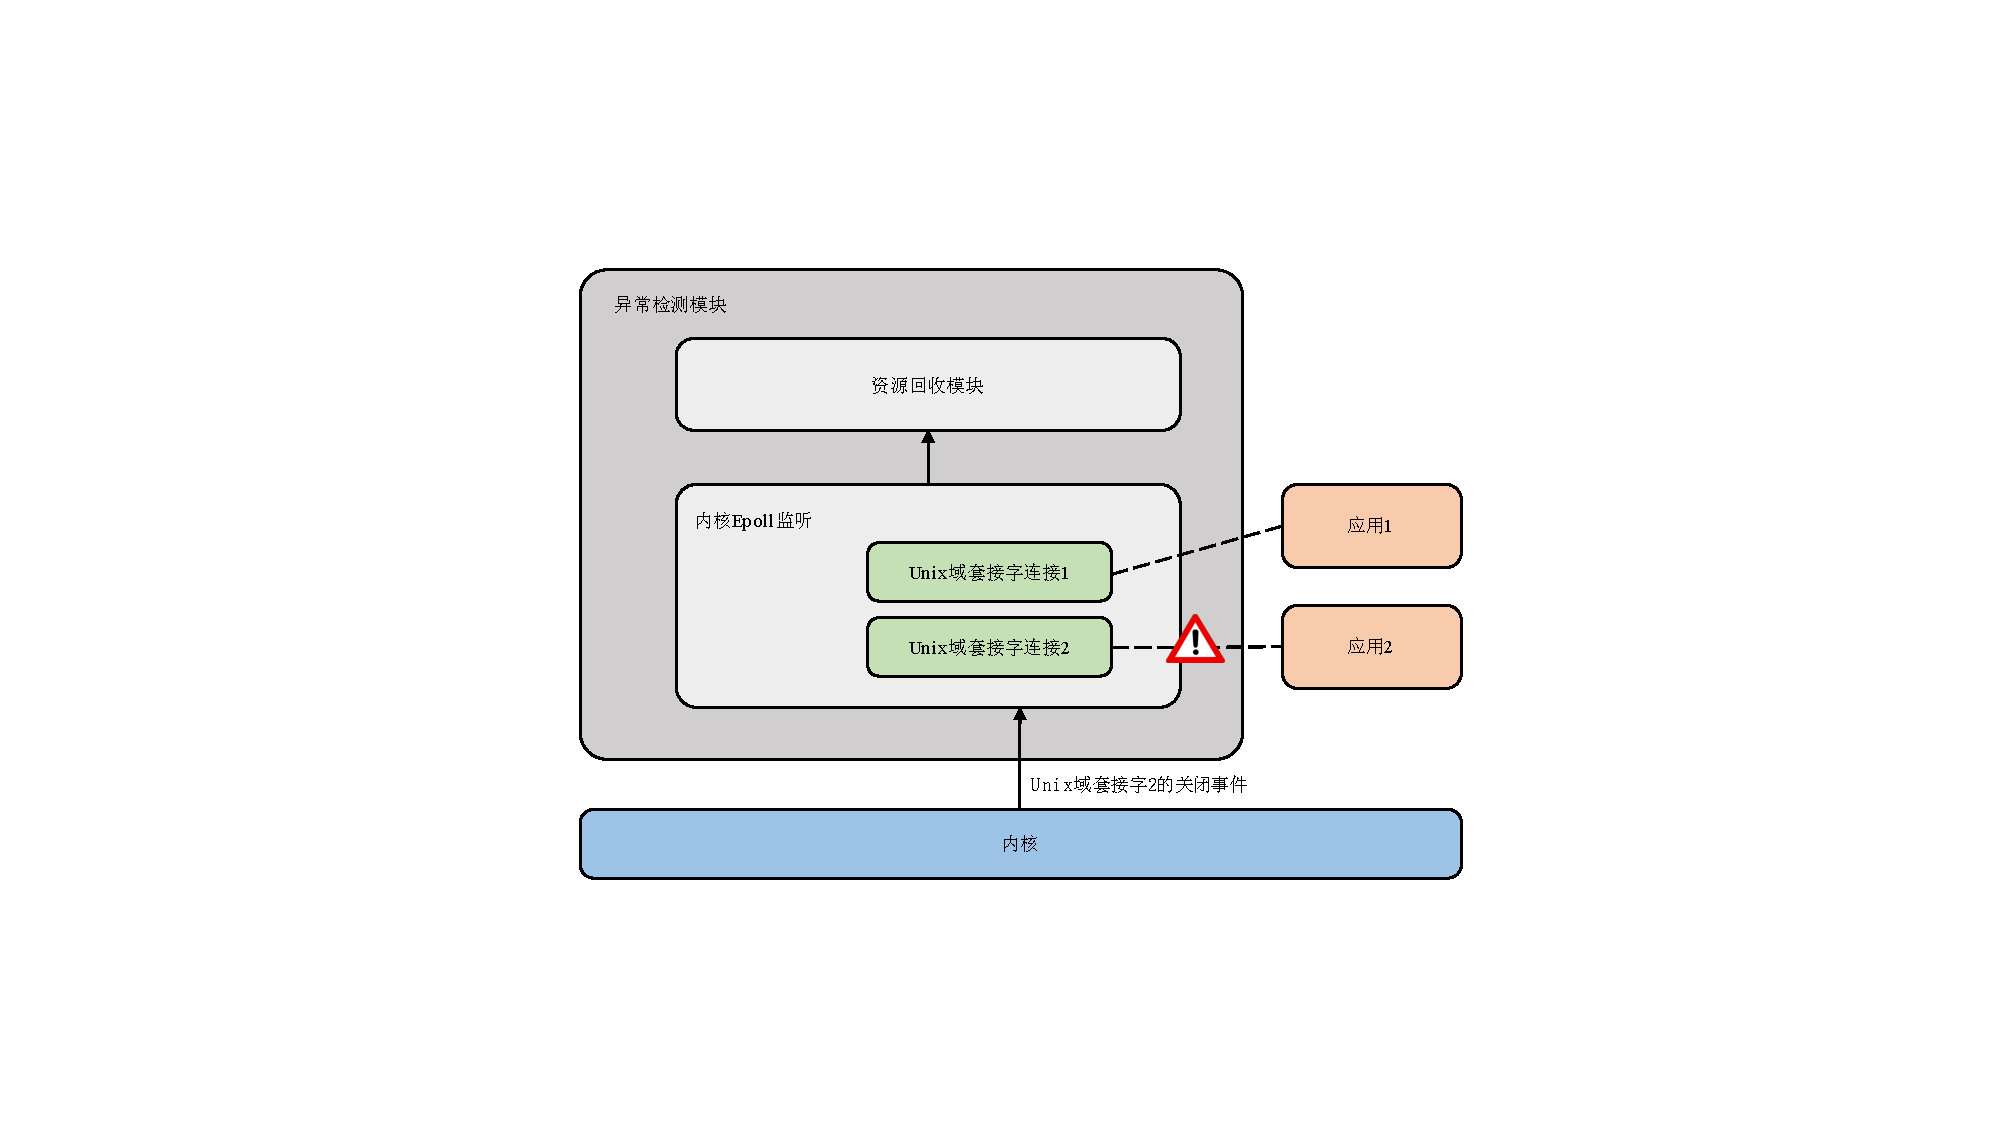
\includegraphics[width=\textwidth]{exception}
  \caption{异常检测模块设计图}
  \label{fig:exception}
\end{figure}
\vspace{-10pt}

异常检测模块的核心是Unix域套接字并利用内核套接字在进程崩溃退出之前会向对端发送FIN包的机制,整个模块的设计思路如图~\ref{fig:exception}所示,当用户态协议栈初始化时会创建一个监听Unix域套接字,在某端口等待本地其他套接字的连接,并用内核epoll监听该Unix域套接字的EPOLL\_CTL\_DEL事件。而当网络应用动态链接到用户态协议栈进行初始化时会创建一个主动连接的内核套接字,调用connect函数与本地Unix域监听套接字建连,这样就在网络应用进程与其对应的用户态协议栈进程中建立套接字通信管道。当网络应用进程崩溃后,其内核套接字会自动向Unix域监听套接字发送FIN包关闭该连接,而用户态协议栈后端在轮询中会定期检查异常检测模块中的内核epoll事件,当协议栈进程收到该FIN包后,协议栈异常检测模块的epoll\_wait返回EPOLL\_CTL\_DEL事件,并根据其文件描述符确定哪个应用异常退出,接下来会将这些信息传递到资源回收模块,对用户态套接字和文件描述符资源进行回收。

该机制对于网络应用线程异常崩溃是无法生效的,因为内核文件描述符在进程地址空间被多个进程共享,即使一个线程退出,也不会出发该内核文件描述符向所有对端发送FIN包。而对于线程池类型的服务,一个线程由于常驻系统中,对其管理的资源进行回收也是很有必要的。而本系统利用pthread\_cleanup\_pop、pthread\_cleanup\_push函数并对pthread\_create函数进行接管,再次封装其主回调函数将资源回收的相关函数加入pthread的cleanup栈中,这样当该线程异常退出后,便会执行该资源回收回调函数。这样便可完成网络应用线程的异常退出资源回收,不过该方案对于thread per request多线程模型代价过大,而每新来一个连接便创建一个线程来处理,这种短生命周期的线程由于发生异常崩溃的几率很小,所以该机制对于短生命周期的执行流可根据用户配置进行关闭。
\chapter{用户态协议栈的兼容性实现}
本工作是偏向工程的系统实现,而本章将从三个角度对用户态协议栈兼容性方面的工程实现进行详细阐述,主要包括协议栈关键结构的设计与实现、协议栈工作主流程和向上对接应用的前端模块的实现细节。

\section{协议栈关键结构的实现}
整个系统的运行流程是基于一个一个关键的数据结构单元,本小节先对本系统中涉及到所有的关键结构进行细分介绍,这些数据结构常常被协议栈和网络应用频繁读写,并且是进程间通信的数据单元,其实现的优劣决定该用户态网络协议栈的性能高低。下面将从网络相关结构体、资源管理结构两个方面进行介绍。
\subsection{用户态套接字结构体的实现}
套接字在内核中的实现结构体有socket和sock两种,两者通过结构体指针互相索引建立一一对应的关系,而两者其实是对同一个套接字连接状态在不同层面的体现,socket作为与网络应用直接对接且是虚拟文件系统inode结点联合体中的一种表示,sock只是针对协议栈传输层网络相关的数据集合,由于网络相关字段过于庞大直接作为inode联合体会造成较为严重的内存浪费,所以内核操作系统将套接字概念进行了区分。在本用户态协议栈中也采取对套接字概念进行区分的策略,分别针对整个系统的三个大模块协议处理模块、后端模块、前端模块定义了socket、backend\_socket、frontend\_socket三种结构体,socket结构体在原Linux内核中的socket结构体基础上进行修改,backend\_socket结构体主要对DPDK接收发送的数据进行缓存管理,frontend\_socket直接对应网络应用并在针对POSIX语义的实现进行字段的设计,frontend\_socket与backend\_socket也同样通过结构体指针进行一一对应,并以资源池的形式进行预分配、申请与回收,三者的数据结构分别如表~\ref{tab:socket},表~\ref{tab:backend_socket},和表~\ref{tab:frontend_socket}所示。

\begin{table}[]
\centering
\caption{Socket数据结构设计}
\label{tab:socket}
\begin{tabular}{ll}
\toprule[1.5pt]
\textbf{字段名称} & \textbf{功能} \\ 
\midrule[1pt]
state & socket所处的状态,包括未分配、未连接、已连接等 \\ 
type & socket的类型,包括UDP数据段、TCP数据流、Raw socket等\\ 
read\_queue\_entry & socket可读事件缓冲队列 \\ 
write\_queue\_entry & socket可写事件缓冲队列 \\ 
accept\_queue\_entry & socket新建连接事件缓冲队列 \\ 
close\_queue\_entry & socket关闭连接事件缓存队列 \\
buffer\_available\_queue\_entry & 接收缓存空间已满事件队列 \\ 
sk & sock结构体指针,与socket结构体建立一一对应关系 \\
ops & proto\_ops结构体指针,由回调函数组成的集合 \\
\bottomrule[1.5pt]
\end{tabular}
\end{table}

\begin{table}[]
\centering
\caption{backend\_socket结构设计}
\label{tab:backend_socket}
\begin{tabular}{ll}
\toprule[1.5pt]
\textbf{字段名称} & \textbf{功能} \\ 
\midrule[1pt]
ring\_idx & 后端socket资源池对应数组的下标,与文件描述符资源一一对应 \\
recv\_ring & DPDK循环队列rte\_ring结构体指针,表示接收端数据报文的缓存 \\
send\_ring & DPDK循环队列rte\_ring结构体指针,表示发送端数据报文的缓存 \\
app\_pid & 表示该socket所属进程的pid,用于进程间socket隔离增加安全性\\
socket & socket结构体指针,并与其一一对应 \\
\bottomrule[1.5pt]
\end{tabular}
\end{table}

\begin{table}[]
\centering
\caption{frontend\_socket结构设计}
\label{tab:frontend_socket}
\begin{tabular}{ll}
\toprule[1.5pt]
\textbf{字段名称} & \textbf{功能} \\ 
\midrule[1pt]
ring\_idx & 前端socket资源池对应数组的下标,与文件描述符资源一一对应 \\
local\_ipaddr & 监听文件描述符的IP地址 \\
local\_port & 监听文件描述符的网络端口 \\
is\_nonblock & 原子布尔变量,代表是否该socket为阻塞式的\\
send\_timeout & 发送数据的超时时间,用于阻塞式发送API实现\\
recv\_timeout & 接收数据的超时时间,用于阻塞式接收API实现 \\
ep\_sock\_lock & DPDK提供的读写锁,用于IO多路复用并发对监听文件描述符进行同步 \\
ep\_node\_list & DPDK提供的读写锁,用于IO多路复用并发对epoll\_node结构的操作进行同步 \\
is\_multicore & 原子布尔变量,表示该监听文件描述符是否为并发监听模式 \\
copies & 整形数组,用于并发监听模式下多个监听描述符之间的互相索引查找 \\
\bottomrule[1.5pt]
\end{tabular}
\end{table}

\subsection{Epoll结构体的实现}
Epoll是Linux内核2.6版本推出的高效IO多路复用机制,也是目前效率最高、使用率最高的网络编程模型,所以本系统针对Epoll实现了三类主要的数据结构,分别是epoll\_event\_info、userspace\_epoll\_node、userspace\_epoll。epoll\_event\_info是作为网络事件的表示单元,后端接收的网络事件均以epoll\_event\_info的形式传送到ready\_connections环形队列中,并向前端内核epoll监听的有名管道写数据而唤醒前端获取这些网络事件。userspace\_epoll\_node是用户态epoll结点单元,在用户态epoll\_ctl被调用后为网络套接字创建新监听事件的时候,将该epoll结点插入到对应socket的epoll\_list中,这是因为一个套接字会存在着被多个epoll进行监听的情况。userspace\_epoll作为前后端IO复用实现的最关键结构体,对应一个预先申请的epoll文件描述符,并且通过DPDK提供的rte\_mempool和rte\_ring实现epoll资源池,在epoll\_create时候进行资源的申请,在epoll\_close时候进行资源的回收。由于rte\_ring环形队列无法进行索引的问题,前端专门对userspace\_epoll进行一次封装定义为frontend\_epoll结构体,并由frontend\_epoll结构体数组的下标在时间复杂度$O(1)$下对epoll进行查找,frontend\_epoll结构体中既包含与其对应的userspace\_epoll结构体指针,还有一个链表与红黑树结合的socket集合,用于高效解决监听的网络套接字事件的查找、删除和添加。具体这三类数据结构的设计如表 ~\ref{tab:epoll_event},表~\ref{tab:epoll_node}和表~\ref{tab:epoll}所示。

\begin{table}[]
\centering
\caption{userspace\_epoll\_node结构设计}
\label{tab:epoll_node}
\begin{tabular}{ll}
\toprule[1.5pt]
\textbf{字段名称} & \textbf{功能} \\
\midrule[1pt]
epoll\_id & 用户态epoll在资源池所对应数组的下标号 \\
epoll\_event & 位掩码表示的正在监听的事件集合 \\
ready\_event & 位掩码表示的已经返回给前端的事件集合 \\
ep\_data & 用户态epoll\_data结构体 \\
entry & epoll结点构成的无锁链表 \\
prev\_node & epoll结点无锁链表的上一个结点 \\
next\_node & epoll结点无锁链表的下一个结点 \\
\bottomrule[1.5pt]
\end{tabular}
\end{table}

\begin{table}[]
\centering
\caption{epoll\_event\_info结构设计}
\label{tab:epoll_event}
\begin{tabular}{ll}
\toprule[1.5pt]
\textbf{字段名称} & \textbf{功能} \\ 
\midrule[1pt]
sockfd & 待响应事件的文件描述符 \\
event & 待响应事件的位域标识符 \\
\bottomrule[1.5pt]
\end{tabular}
\end{table}

\begin{table}[]
\centering
\caption{userspace\_epoll结构设计}
\label{tab:epoll}
\begin{tabular}{lp{10cm}}
\toprule[1.5pt]
\textbf{字段名称} & \textbf{功能} \\ 
\midrule[1pt]
epoll\_id & 用户态epoll在资源池所对应数组的下标号 \\
is\_sleeping & 表示当前用户态epoll是否出于睡眠睡眠 \\
ep\_lock & DPDK提供的读写锁,用于同步用户态epoll结点链表的读写操作 \\
kernel\_epoll\_fd & 用户态epoll所对应的内核epoll文件描述符 \\
epoll\_events & 非网络事件待响应数组 \\
fifo\_write\_fds & 后端在事件响应后写入的有名管道数组 \\
fifo\_read\_fds & 前端模块内核epoll监听的有名管道数组 \\
app\_pid & 用户态epoll所对应的进程pid,用于安全检测 \\
shadow\_connections & DPDK提供的循环队列rte\_ring结构体指针,缓存每次事件聚合操作后剩余的epoll事件 \\
ready\_connections & DPDK提供的循环队列rte\_ring结构体指针,缓存每次事件聚合返回给前端的事件 \\
\bottomrule[1.5pt]
\end{tabular}
\end{table}

\subsection{资源管理结构的实现}

本系统协议栈进程与网络应用进程分核的设计模式导致在前后端两进程中有大量的数据需要共享以及相关信息需要传递,这对整个系统的性能起着重要作用,共享资源的管理核心是资源预分配,因为用户态socket和用户态epoll这些资源需要频繁地申请与释放,预分配的优势在于最大程度地避免频繁申请与释放带来的性能开销,但其劣势在于一旦并发过高导致资源池不够用网络应用就无法继续服务,所以需要设定合理的资源预分配初始值,Redis应用默认的最大同时并发数是1024个,而本用户态协议栈系统采用该数值的两倍来作为资源预分配的初始值,可以满足绝大部分网络应用使用场景。

前后端进程共享资源的实现都是利用DPDK提供的rte\_ring和rte\_mempool来实现的,rte\_mempool通过DPDK大页内存来实现,并且rte\_ring提供了基于CAS实现的无锁模式,适用于单生产者单消费者、多生产者多消费者等各种模式,所以其入队、出队操作的效率也较高。本系统为了支持网络应用多进程等并发流的多核扩展,所以将共享资源分为每个协议栈进程独占的资源和所有协议栈进程共享的资源,前者通常使用在command这种存在大量消息传递的场景,单生产者单消费者的效率较高,具体如下表~\ref{tab:onecore}和表~\ref{tab:multicore}所示,在此仅列出rte\_mempool资源池,理应都会有一个rte\_ring循环队列与其对应,作为申请与回收资源指针的获取入口,在此不予赘述。

本系统的资源都是放在DPDK配置的大页内存中进行管理,通过rte\_ring和rte\_mempool实现资源池管理模式,而前后端最重要的信息传递通道包括由前端向后端传递的命令消息,即表~\ref{tab:onecore}中的command\_ring消息队列中的信息单元,而command结构中有包含各种命令的联合体,如表~\ref{tab:command}所示。此外还有从后端向前端传递的网络事件消息,即通过ready\_connections消息队列来完成的,接下来按照一个完整的epoll网络服务器建立通信过程的顺序对命令消息的种类进行一一介绍。

US\_OPEN\_SOCKET\_COMMAND: 当网络服务器调用用户态socket申请创建一个新socket的时候,协议栈前端直接从用户态socket资源池中获取一个socket资源并将其各字段初始化,此时由于并不知道该socket是否为监听socket所以并没有将用户态socket与内核态sock结构体进行绑定,这样可以在主动连接情况下避免过多内存资源的损耗。当网络应用调用用户态bind进行内核端口绑定时候,由于协议栈前端无法对内核资源进行相关操作,所以从command资源池中申请一个command结构体并复用成为US\_OPEN\_SOCKET\_COMMAND,当该命令传递到后端时会创建真正的内核sock结构体,并调用内核相关函数将该socket的family和type值赋予到内核sock中,从而完成了前后端socket结构体的lazy模式绑定。

US\_BIND\_SOCKET\_COMMAND: 当网络应用调用用户态bind函数对该socket的sockaddr相关信息进行设置,比如绑定对应端口等,由于sockaddr相关信息在后端sock结构体中,所以前端从命令资源池中申请一个command并复用为US\_BIND\_SOCKET\_COMMAND,将网络应用传递的sockaddr相关信息传递到后端,当后端收到该命令时便会调用移植的kernel\_bind函数从而完成相关设置。

US\_CONNECT\_SOCKET\_COMMAND:当网络应用调用用户态connect函数,其参数类型与bind函数一样具有sockaddr相关信息,由于sockaddr相关信息在后端sock结构体中,所以依然需要前端从命令资源池中申请一个command并复用为US\_CONNECT\_SOCKET\_COMMAND,将网络应用传递的sockaddr相关信息传递到后端,当后端收到该命令时便会调用移植的kernel\_bind与kernel\_connect函数从而完成相关设置。

US\_SETSOCKOPT\_COMMAND: Linux内核中的socket套接字一直存在着各种属性值,比如对TCP长连接和内核缓冲队列的相关配置等都是通过setsockopt该系统调用来完成的,本系统也对setsockopt系统调用进行了劫持,但是由于协议栈前端无法完成对sock结构体的相关配置,所以当网络应用在创建完一个socket之后调用用户态setsockopt进行相关属性设置时候,前端就会申请一个command并复用为US\_SETSOCKOPT\_COMMAND,当后端收到该命令后,会调用移植的内核sock\_setsockopt进行真正的socket属性配置,从而完成用户态协议栈对socket属性值的设置功能。

US\_LISTEN\_SOCKET\_COMMAND: 当网络应用调用用户态listen对该socket进行监听化并设置其监听队列的backlog,同样由于backlog的设置必须在后端模块完成,所以前端会申请一个command结构体并复用为US\_LISTEN\_SOCKET\_COMMAND,将其传递到command\_ring消息队列中,当后端模块轮询到该命令后,便会间接调用移植的内核kernel\_listen函数对该socket进行监听队列的相关配置。这样网络应用便完成了一个监听socket的创建、设置以及前后端绑定的过程。

US\_EPOLL\_CREATE\_COMMAND: 本系统epoll事件的通知机制是由内核epoll和有名管道实现,有名管道作为前后端进程间通信触发控制信息的通道必须在前后端同时进行open才能完成通信,所以当网络应用调用用户态epoll\_create时前端会从command资源池中申请一个command结构体并复用为US\_EPOLL\_CREATE\_COMMAND,其中包含epoll\_id和进程pid等消息,当后端收到该命令后便根据前端传来的这些信息拼凑出有名管道的名称从而在后端打开该管道,这样才能在事件待响应时通过在后端写有名管道来完成前端内核epoll\_wait的唤醒。

US\_SET\_SOCKET\_RING\_COMMAND: 该命令发生在网络服务器创建监听socket并用epoll进行监听之后,网络客户端开始不断向网络服务器发起请求,当协议栈后端通过DPDK轮询接收到TCP SYN包,通过协议处理模块完成整个TCP三次握手过程,并将待响应事件插入到前端可以接收的消息队列中,并唤醒前端的epoll\_wait,此时前端若判断待响应socket文件描述符为监听类型,便得知有新建连接到来,进一步调用用户态accept函数进行创建新套接字去完成与该客户端的读写过程,由于后端在向前端传递事件时候需要与前端socket进行绑定且已知其ring\_idx等相关信息,所以在用户态accept被调用之后,前端会从command资源池中申请一个command结构体并复用为US\_SET\_SOCKET\_RING\_COMMAND,在后端收到该命令之后便会对backend\_socket结构体的ring\_idx、apppid和socket等字段进行设置,并与前端套接字进行指针互绑定,最终调用新建连接事件的通知回调函数去经过事件聚合后完成对前端内核epoll\_wait的唤醒。所以US\_SET\_SOCKET\_RING\_COMMAND实现了前后端socket信息绑定以及触发事件通知的功能。

US\_RECV\_SOCKET\_COMMAND: DPDK通过轮询IO模式不断将数据包读取到socket结构体中的iovec结构中,iovec是移植后数据包存储的形式,并结合DPDK提供的rte\_mbuf结构体来实现,iovec结构体中存放的数据不可能无限增长,必须由后端在合适的时机将其数据传递到前端并进行网络应用逻辑处理从而最后完成释放,US\_RECV\_SOCKET\_COMMAND命令就是本系统接收数据包并传递到网络应用buffer中的关键。当网络应用调用用户态收包recv、read等接口,此时就应该通知后端对iovec结构中的数据包进行向前端传递的操作,此时便在command资源池中申请一个command结构体并复用为US\_RECV\_SOCKET\_COMMAND。当后端接收到该命令并完成前后端套接字绑定校验后,会调用移植的kernel\_recvmsg函数将该套接字iovec中的rte\_mbuf数据包推送到前端数据接收缓冲队列中,该过程是数据的指针传递并不涉及数据的内存拷贝。在成功完成向前端传递packet指针后便会调用数据待接收事件回调函数并进行有名管道的写操作,从而唤醒前端内核epoll\_wait。当前端检查到该socket存在数据待接收,便调用recv进行数据接收。由于recv等接口中存在网络应用创建的buffer,则rte\_mbuf中的报文数据就不得不经过一次数据拷贝才能复制到网络应用缓冲区中,这是由于POSIX语义造成无法实现真正的零拷贝。


US\_SEND\_SOCKET\_COMMAND: 在前端的网络应用数据必须传递到后端才能通过DPDK发送出去,所以发送数据依然无法避免前后端的通信。当网络应用调用send、write等相关用户态发送接口后,前端会将根据缓冲区的大小与MTU最大传输单元将应用数据装配到一个一个rte\_mbuf中,并传递到后端发送队列中,接下来会从command资源池中申请一个command结构体并复用为US\_SEND\_SOCKET\_COMMAND,将ring\_idx等信息赋予其中,然后传递到命令队列中。当后端轮询到该命令之后,便会调用发送数据包事件回调函数,调用移植的kernel\_sendpage并最终通过DPDK发送数据的接口将数据包发送到网卡队列中。

US\_CLOSE\_SOCKET\_COMMAND: 由于用户态网络socket在前后端管理着各种各样的资源,当该socket被网络应用确认关闭后,就必须在前后端都对相关资源进行释放和回收,防止内存泄漏的发生。当网络应用调用用户态close接口时,前端会释放其管理的资源,并从command资源池中申请一个命令并复用为US\_CLOSE\_SOCKET\_COMMAND。当后端轮询到该命令后,会将后端socket管理的接收、发送缓冲队列、用户态socket等资源全部释放并回收给资源池,并将后端模块与协议处理模块之间的read\_queue\_entry、write\_queue\_entry、accept\_queue\_entry、close\_queue\_entry队列中的元素全部出队,以便用户态socket可以复用,并最终调用移植的kernel\_close对sock结构体进行释放。

\begin{table}[]
\centering
\caption{单个协议栈进程独享的资源}
\label{tab:onecore}
\begin{tabular}{lp{10cm}}
\toprule[1.5pt]
\textbf{资源名称} & \textbf{详细介绍} \\ 
\midrule[1pt]
command\_ring & 用于前后端传递控制命令的重要通道 \\
free\_command\_pool & 可用的命令结构体资源,初始值大小32768  \\
free\_return\_value\_pool & 用户态POSIX API返回值结构体资源池,初始值大小32768 \\
\bottomrule[1.5pt]
\end{tabular}
\end{table}

\begin{table}[]
\centering
\caption{多个协议栈进程共享的资源}
\label{tab:multicore}
\begin{tabular}{lp{10cm}}
\toprule[1.5pt]
\textbf{资源名称} & \textbf{详细介绍} \\ 
\midrule[1pt]
free\_event\_info\_pool & 可用的epoll事件信息共享内存资源池,多消费者多生产者模式,资源池初始大小为65536 \\
free\_epoll\_node\_pool & 可用的epoll结点共享内存资源池,多消费者多生产者模式,资源池初始大小为32768  \\
free\_connections\_pool & 可用的用户态socket结构体共享内存资源池,资源池初始大小为2048,与g\_sockets全局数组进行关联 \\
epolls\_pool & 可用的用户态epoll结构体共享内存资源池,资源池初始大小为64,在前端与g\_epolls全局数组进行关联 \\
\bottomrule[1.5pt]
\end{tabular}
\end{table}

\begin{table}[]
\centering
\caption{前后端消息单元command结构体}
\label{tab:command}
\begin{tabular}{lp{10cm}}
\toprule[1.5pt]
\textbf{资源名称} & \textbf{详细介绍} \\ 
\midrule[1pt]
command\_id & command种类ID号,具体command由枚举定义 \\
ring\_idx & 相关联用户态socket对应其g\_sockets的数组下标 \\
return\_value & 返回给前端的返回值结构体指针 \\
command\_union & 存放各种command结构体内容的联合体,包含10多种command结构体 \\
\bottomrule[1.5pt]
\end{tabular}
\end{table}

\section{协议栈工作主流程实现}

整个系统由协议处理模块、后端模块、前端模块组成并采用协议栈进程与网络应用进程分核的设计理念,将这些各个模块、各个进程协调去完成各种网络模型的功能已是有挑战性的工作,在具体实现上如何兼顾高性能与高兼容更是将系统开发的难度提升一个层次,本节将从协议栈初始化、协议栈主循环和前端模块的实现三个方面对系统从实现角度进行剖析。

\subsection{协议栈初始化}
网络通信过程涉及到众多内存资源的管理,比如套接字资源、文件描述符资源、packet资源、各种缓冲和消息队列等。在高并发高吞吐的网络条件下,这些资源频繁的申请与释放会导致较大的性能开销,所以本系统在初始化过程中重点对各种资源进行预分配管理,并通过资源池的形式对应用提供资源的申请与释放。除此之外,还对相关轮询周期、各种队列进行初始化配置,整个协议栈初始化过程具体如下
\begin{enumerate}[(1),labelsep=.5em, leftmargin = 0pt, itemindent = 3em]
\item 初始化主循环各个处理逻辑的循环周期,首先会根据DPDK获取当前绑定网卡的带宽、当前以太网的MTU和DPDK一次轮询最大接收报文个数,并计算出进行一次DPDK轮询所消耗的时间以此作为DPDK驱动轮询循环周期,然后为定时器轮询、发送队列循环检测、接收队列循环检测和系统异常崩溃检测等这些逻辑设定周期,这决定了主循环中各个处理逻辑真正占用的CPU资源数并对系统性能有着重大影响,比如发送队列循环检测队列如果被设置过小而远超过队列生成速度从而造成CPU资源的无端浪费,而如果设置过大则会造成发送数据报文的大量堆积从而引发连接的延迟过高。除了循环周期的设置,还会调用DPDK提供的rte\_timer定时器为每个协议栈进程对应的DPDK设置时钟校验周期,从而提升主循环处理逻辑分配的准确性。主循环的各个逻辑将在下一小节进行更加详细的阐述。
\item 初始化用户态协议栈的日志系统,整个大系统在开发调试过程中遇到过各种各样的问题与bug,一个合理的日志系统可以帮助调试bug,更好更快地发现和定位问题。该日志系统基于Linux系统的syslog,并将日志分为debug、info、warning、error、critical五个级别,并可以控制日志是利用syslog输出到/var/log的指定路径下的文件还是直接输出到标准输出中。对于系统遇到的常见异常情况都配有warning和error级别的日志进行监控,方便用户及时观测到系统的异常情况。用户态协议栈日志系统的默认配置是输出warning及其以上级别的日志到/var/log指定路径下的文件。
\item 初始化所有进程间通信使用的rte\_ring和rte\_mempool,两者配合使用实现了对所有资源的预分配资源池管理方式,最大程度上减少内存反复申请和释放的性能开销。这些资源中既有单个协议栈进程独享的资源,也有在各个协议栈进程之间共享的。其中对用户态socket和epoll的资源管理模式较为特殊,由于rte\_ring这种消费生产模式不具备索引功能,而前后端对socket和epoll操作和传递信息的时候都需要直接定位到当前操作的socket或epoll,这便需要用数组的索引模式来直接获取。在初始化中对于这类资源初始化一个连续的大页内存,并将用户态socket指针指向大页内存数据的初始地址,然后循环自增用户态socket指针,并对每一块指定的用户态socket进行初始化并放入free\_connection\_ring这个资源池当中,其中每个用户态socket资源本身携带有ring\_idx这个索引字段,这样就可以通过数组索引直接定位到所操作的用户态socket或epoll。
\item 初始化系统异常崩溃检测系统,该系统的实现是基于Unix域socket和epoll实现的,所以在协议栈初始化过程中就需要创建一个监听Unix域套接字,并用内核epoll对其关闭事件进行监听,除此之外在网络应用进程初始化过程中还需要创建一个建连套接字,向对应的协议栈Unix域套接字发起连接,这样当网络应用进程异常退出之后便会向该Unix域套接字发送FIN包,从而触发协议栈内核epoll的事件响应。
\end{enumerate}

\subsection{协议栈主循环详解} %包括事件通知流程图
当协议栈进程完成初始化之后便进入主循环体中,其中包括对command\_ring的处理、DPDK收包、发送缓冲队列处理、接收缓冲队列处理以及系统异常崩溃检测处理,除了命令队列的处理以外其他操作都是以固定的周期进行的,而命令队列为了保证前端传来的命令可以及时得到处理所以每进入一次主循环体都会检查command\_ring并进行相应操作。下面对这些主循环中的操作进行一一详细分析。

命令队列:本文上一节中已经介绍了该用户态协议栈中常见的命令,协议栈进程和网络应用进程分核设计的模式就导致前端一些用户态网络调用需要在后端进行相应的处理,而对命令队列处理属于优先级较高的操作,因为如果前端传递的命令如果没有及时处理,涉及到该网络套接字的后续操作都无法继续进行或者操作失败导致连接断开,但是在高并发高吞吐情况下又不能每次将命令队列里所有命令挨个处理完再进行其他操作,因为这样会导致过多处理时间在命令队列处理而其他一些操作,比如DPDK收包也需要较高的实时性才能保证系统的整体性能。所以命令队列单次处理命令的个数是根据当前其他操作成本而进行动态调整的,本系统设计的动态调整算法基于网络情况通常在一段时间具有连续性的特征,即每次进入循环体会对非命令队列操作处理总时间进行统计,当次命令处理个数与上次非命令队列操作处理时间成负相关,即上次非命令队列操作处理时间越长,说明这次命令队列处理所需要的时间成本就更高,此时命令队列就不能过多占用CPU资源。

DPDK收包:整个系统的报文接收依赖于基于轮询IO的DPDK,用轮询替代中断的收包模式可以减轻在高网络流量下硬件中断对CPU资源带来的压力,当然这就需要对DPDK收包的周期进行合理设置,过小的周期会让CPU白白浪费在无效的轮询收包上,过大的周期又难以保证数据包接收的时效性。DPDK收包最终调用的是DPDK提供的rte\_eth\_rx\_burst接口,它可以完成批量接收数据报文,单次最大接收报文个数在DPDK的配置中由参数MAX\_PKT\_BURST决定,默认设置为32。

发送缓冲队列处理:write\_queue\_entry是后端模块与协议处理模块的重要队列,也是发送数据的一条重要通道,当后端从该队列中出队一个内核sock结构体,会根据sock结构体的类型去调用kernel\_sendpage或者udp\_sendmsg去发送TCP数据或者UDP数据,直到将该队列中的所有待发送数据全部发送完毕。

接收缓冲队列处理:接收到的TCP数据包通常有三类,第一类是新建连接的SYN包,第二类是关闭连接的FIN包,第三类是普通的数据包,而接收缓冲队列的处理就是针对这三类数据包对应的accept\_queue\_entry、close\_queue\_entry和read\_queue\_entry队列进行出队处理。针对accept队列中的元素先在移植的用户态协议处理模块中完成三次握手的处理并最终将新建连接事件插入到前端可以获得的accept消息队列中。针对close队列中的元素则会将该socket所有的发送接收缓存全部清空并回收,并最终调用移植后的kernel\_close函数对协议栈内核sock结构体进行释放。针对read队列中的元素则会调用接收事件回调函数,通过kernel\_recvmsg将iovec中的mbuf数据包发送到前端可接收的read缓冲队列中,并触发相应的socket可读事件。

\subsection{协议栈重要流程分析} %用户态网络API的实现

协议栈系统中由于前后端分离的设计存在着较为复杂的数据与事件信息的交互过程,其中对网络性能影响最大的是接收数据流程和发送数据流程,本小节会对这两种重要流程进行详细分析。

接收数据流程:网络数据从网卡最终到网络应用接收函数调用的buffer在整个用户态协议栈系统中经历的过程如图~\ref{fig:recv}所示。首先在主循环当DPDK收包周期调用被触发,DPDK通过rte\_eth\_rx\_burst函数从网卡队列将数据包接收到用户态程序中,并经过协议处理模块中数据链路层、网络层、传输层的筛选与校验,并将该数据包以rte\_mbuf的形式存放到sock结构体中iovec中,然后将该接收数据包写入到协议处理模块与后端模块的接收通道read\_queue\_entry中。在前后端共享的用户态套接字rx\_ring接收缓冲队列的入队操作是由接收事件回调函数来完成的,而该回调函数的触发方式有两种,一种是由协议处理模块完成数据包接收后来调用,而另一种是由网络应用在前端调用recv等接收函数将接收命令传入command\_ring,并由后端完成对该接收命令的处理后间接调用接收事件回调函数,这样可以双重保证数据包接收到网络应用的实时性。接收方向唯一一次数据拷贝是将大页内存中的数据拷贝到网络应用buffer中,且这次数据拷贝在不修改协议栈API语义的情况下无法避免。

发送数据流程:网络数据从应用调用send等发包函数的buffer到最终到达网卡发送出去在整个用户态协议栈系统中经历的过程如图~\ref{fig:send}所示。首先当网络应用调用send函数时先将buffer中的网络数据组装成多个mbuf结构体,并入队进前后端共享的用户态套接字tx\_ring发送缓冲队列中,此外还将发送数据命令入队到前后端共享的command\_ring当中。当后端模块轮询到该发送数据命令后,会调用发送事件回调函数并通过协议处理模块的kernel\_sendpage函数将数据通过传输层、网络层、数据链路层向下传递到DPDK的发送驱动模块中,最终通过DPDK的rte\_eth\_tx\_burst函数将该网络数据以mbuf形式发送出去,发送方向的唯一一次数据拷贝同样是为了兼容POSIX API语义而无法避免的。

\vspace{-10pt}
\begin{figure}[H] % use float package if you want it here
  \centering
  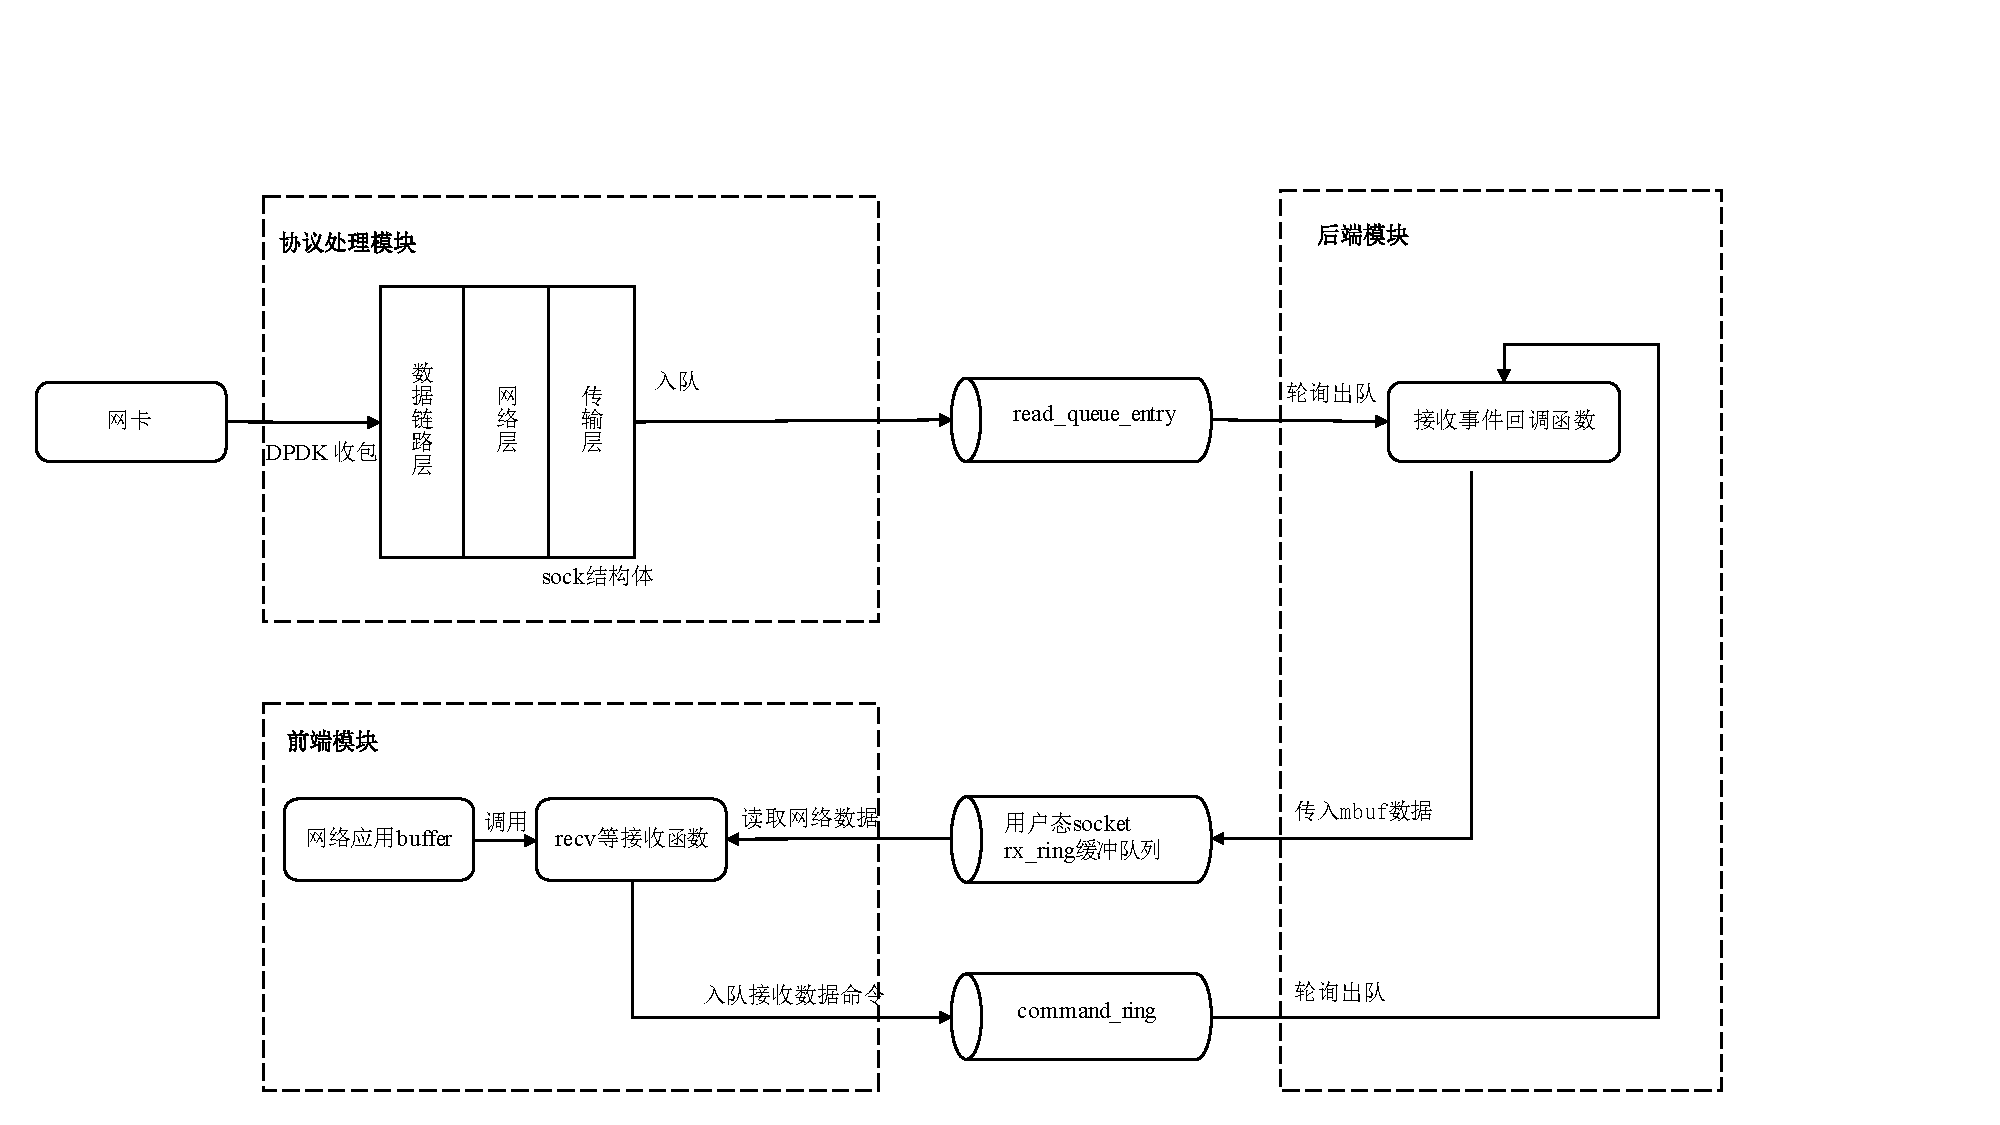
\includegraphics[width=\textwidth]{recv}
  \caption{用户态协议栈数据接收流程}
  \label{fig:recv}
\end{figure}
\vspace{-10pt}

\vspace{-10pt}
\begin{figure}[H] % use float package if you want it here
  \centering
  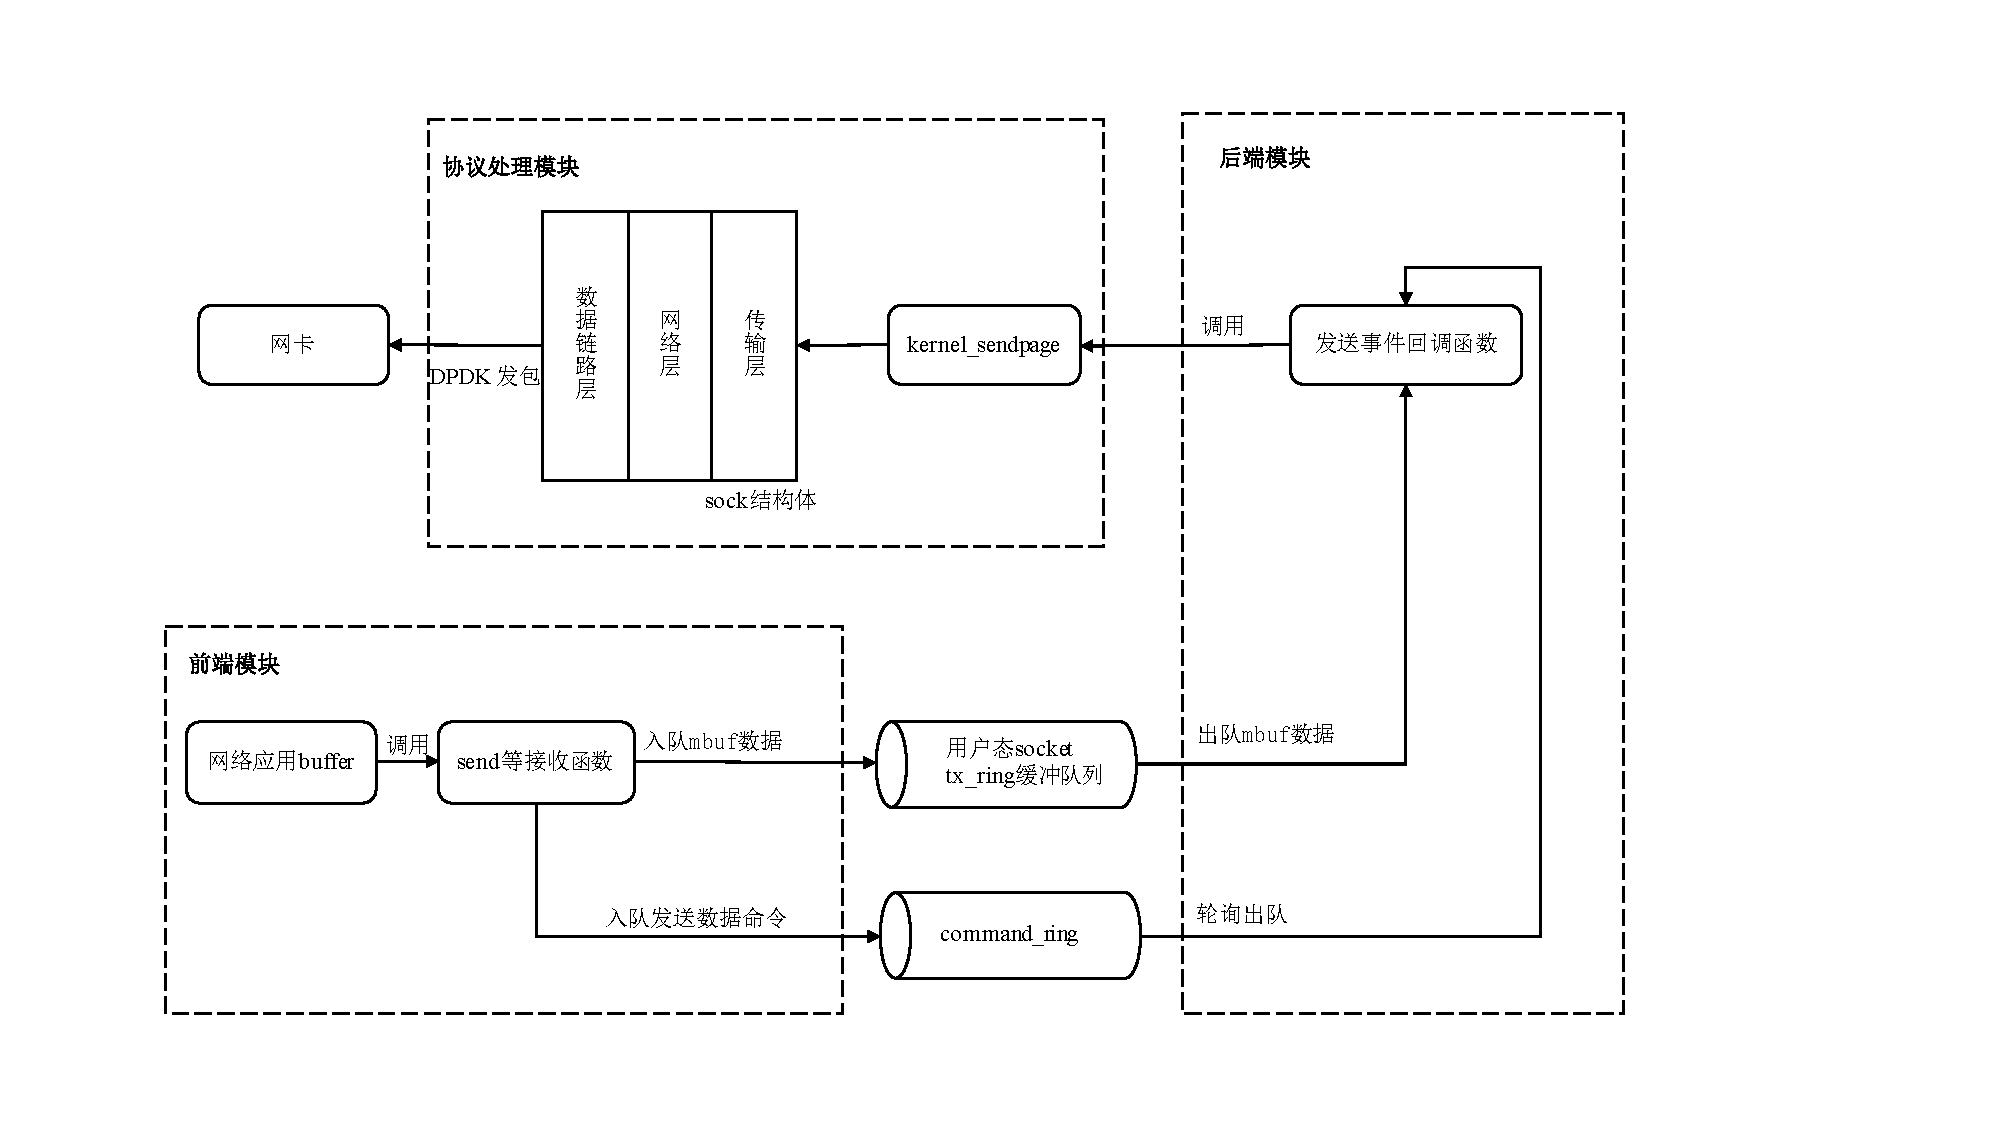
\includegraphics[width=\textwidth]{send}
  \caption{用户态协议栈数据发送流程}
  \label{fig:send}
\end{figure}
\vspace{-10pt}
\chapter{实验结果与分析}

整个用户态协议栈系统工程量是21386行代码,其中包含移植后的Linux内核网络协议栈。启动网络应用之前,需要先在后台运行用户态协议栈进程,根据用户配置的进程个数和CPU核掩码,用户态协议栈进程以100\%的CPU占用率独占专用的CPU核。此外前端模块通过GCC编译成为动态链接SO库,接下来就可以启动网络应用服务器进程,等待客户端进行网络连接请求。在完成对整个系统的设计与开发实现后,就需要对多种主流网络应用进行移植,并且在保证不修改网络应用任何源码的前提下获得网络性能的提升。本章首先对实验环境的搭建进行简介,然后对移植后的Nginx、Lighttpd、Redis网络应用与4.15版本Linux内核的网络性能进行对比,重点关注网络延迟和吞吐。

\section{实验环境配置}
实验环境的搭建主要由三台高性能网络服务器和一台光交换机组成,实验拓扑如下图~\ref{fig:topo}所示,其中高性能网络服务器的配置均采用10Gb 82599ES Intel网卡,志强E5系列2.1Ghz主频的CPU,光交换机的配置是Mellanox公司生产的SN2100系列16端口100Gb带宽,两台服务器作为客户机与光交换机通过光纤直连,一台服务器作为运行网络应用作为服务器等待客户连接并与光交换机通过光纤直连。

\vspace{-10pt}
\begin{figure}[H] % use float package if you want it here
  \centering
  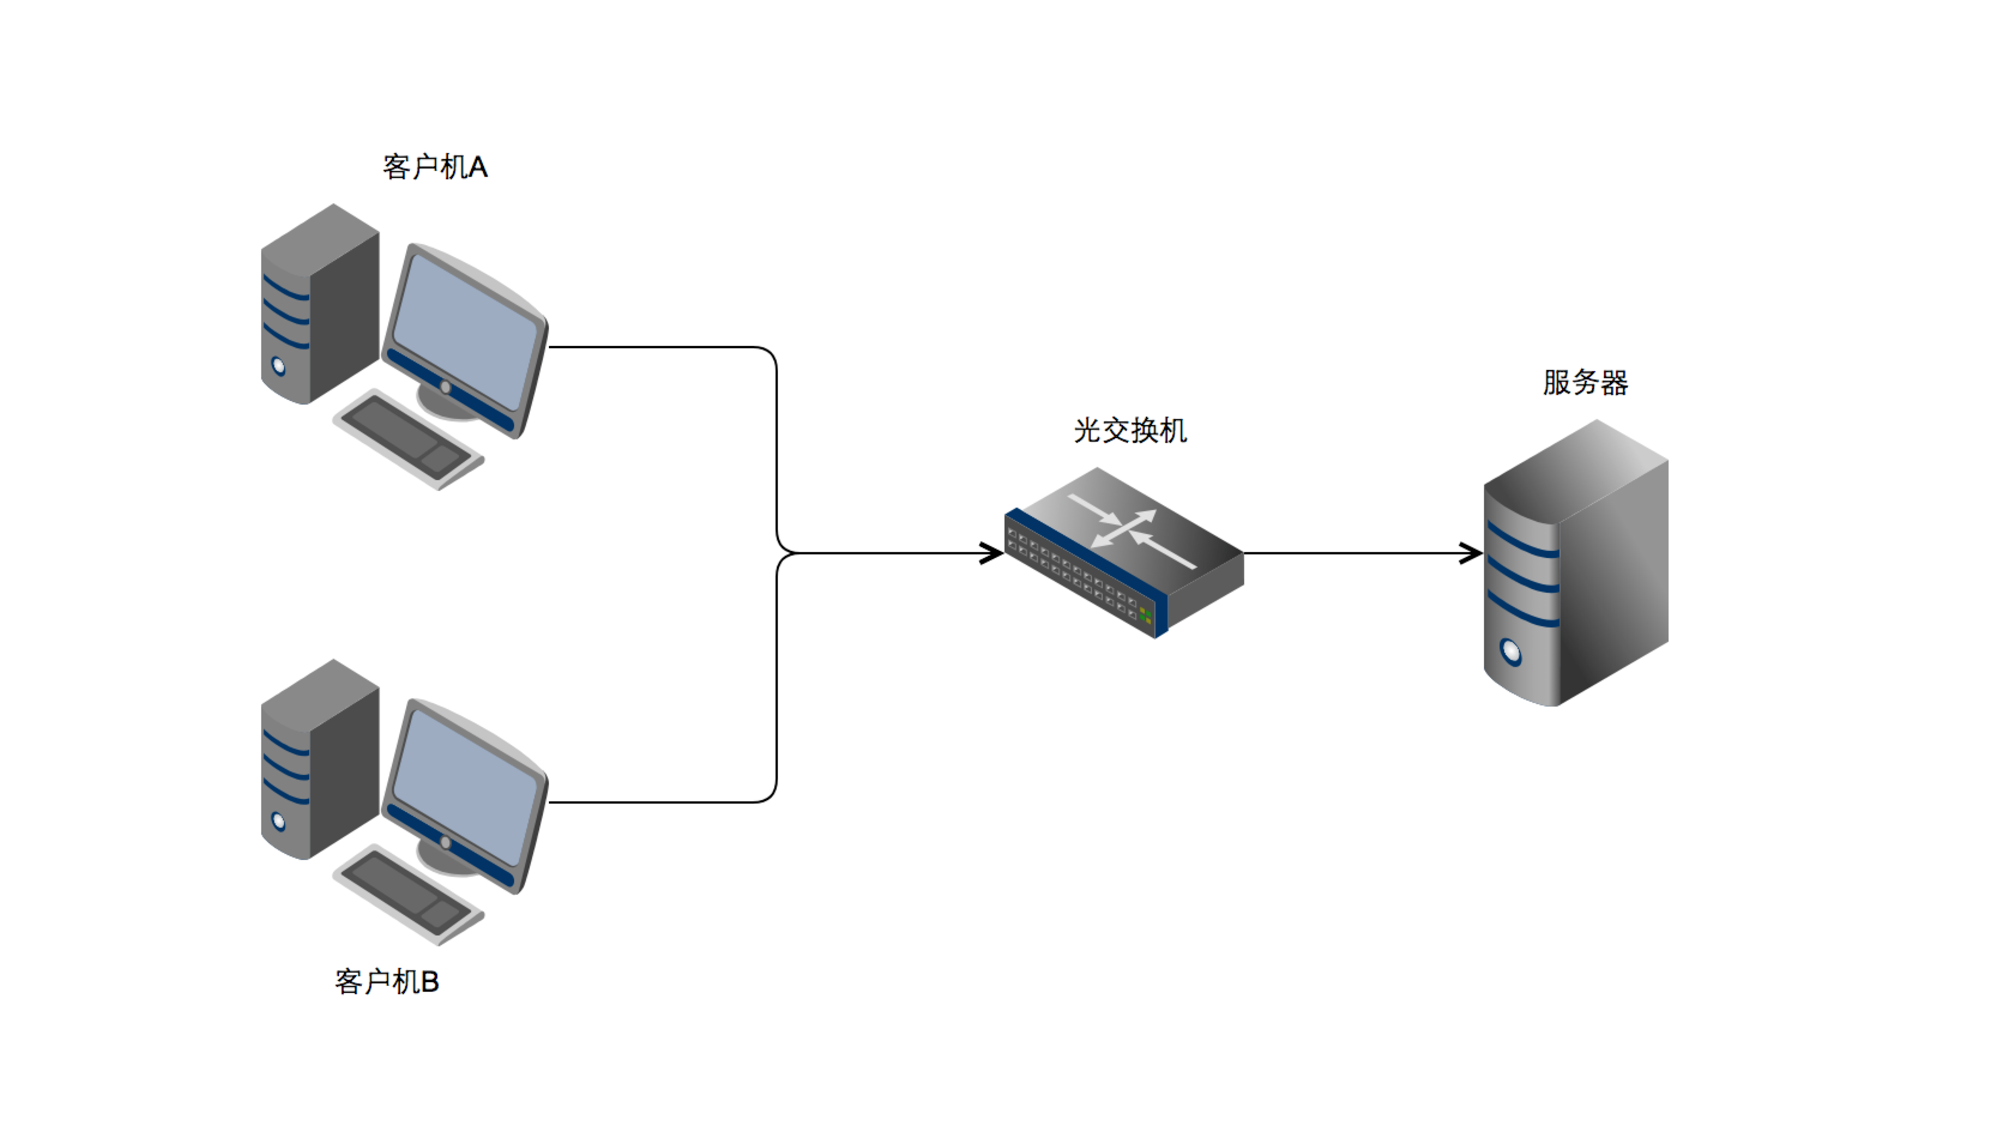
\includegraphics[width=\textwidth]{topo}
  \caption{实验环境拓扑图}
  \label{fig:topo}
\end{figure}
\vspace{-10pt}

网络应用所在服务器采用Ubuntu14.04、16.04和18.04均能完成应用的成功移植。为保证对比最新的基准,Linux使用经过零拷贝等优化的4.15内核版本,实验测试最终三台网络服务器都采用18.04版本的Ubuntu系统。实验性能本应该与同样具备应用兼容性的高性能用户态协议栈Fastsocket进行,不过按照其官网教程~\cite{fastsocket-release}进行配置后其运行性能远远低于论文中的性能,向论文作者寻求帮助后依然没有将其性能进行复现。此外,对于具备POSIX-Like API的用户态协议栈mTCP和F-stack,由于它们都移植了Lighttpd这款网络应用,所以本文为与其进行性能对比而移植Lighttpd。IX、ZygOS由于API语义完全脱离传统POSIX API并且其官方没有给出主流网络应用的移植实验成果,所以本文就未与其进行实验对比。综上所述,本章移植Nginx、Redis并与Linux 4.15版本内核网络协议栈进行性能对比,移植Lighttpd同时与Linux 4.15版本、mTCP进行性能对比。
\section{Nginx实验结果}
Nginx~\cite{Nginx}是当前最为广泛使用的Web应用服务器,既可以用来作为静态资源服务器,又可以做反向代理,利用Epoll实现在较低服务器资源消耗下达到高并发网络处理,其支持单进程运行和多进程主从运行两种模式。本用户态协议栈对两种运行模式都予以支持。在移植初期为保证Nginx服务器运行正常,通常采用两台机器直连,一台作为服务器,另一台作为客户机,在客户机使用wget进行Nginx网络连通性测试,并检测下载得到的静态文件是否正确来验证Nginx是否成功工作。

在保证Nginx运行无误后,为了模拟高并发高吞吐的网络环境,本实验在如图~\ref{fig:topo}的环境下,在两台客户机上同时使用wrk~\cite{wrk}benchmark工具,开启64个线程、512个并发连接进行1分钟的压力测试,在服务器上分别基于4.15版本Linux内核协议栈和本用户态协议栈运行1.9.5稳定版本的Nginx。由于本系统采用协议栈进程与网络应用进程分核的设计方式,即Nginx网络worker进程与用户态协议栈进程是成对出现的,所以实验使用的CPU核数是两核、四核、六核、八核、十核这五种。为了保证实验公平性,通过BIOS只开启对应的物理核,并且用户态协议栈两核(一个协议栈进程+一个Nginx worker进程)的性能是与Linux网络协议栈(两个Nginx worker)进行对比,因为二者所占用的CPU资源数是一样的。此外,实验将Nginx的keepalive时间设置为0,即一次TCP完整连接只进行一次静态文件的请求与响应,并且静态文件的大小统一设置为64B,这是为了模拟真实网络环境中的短连接。在这样的环境配置下进行实验得到如下用户态协议栈与Linux内核协议栈吞吐对比图~\ref{fig:NginxRPS}以及平均延迟对比图~\ref{fig:NginxAvg}。

\vspace{-10pt}
\begin{figure}[H] % use float package if you want it here
  \centering
  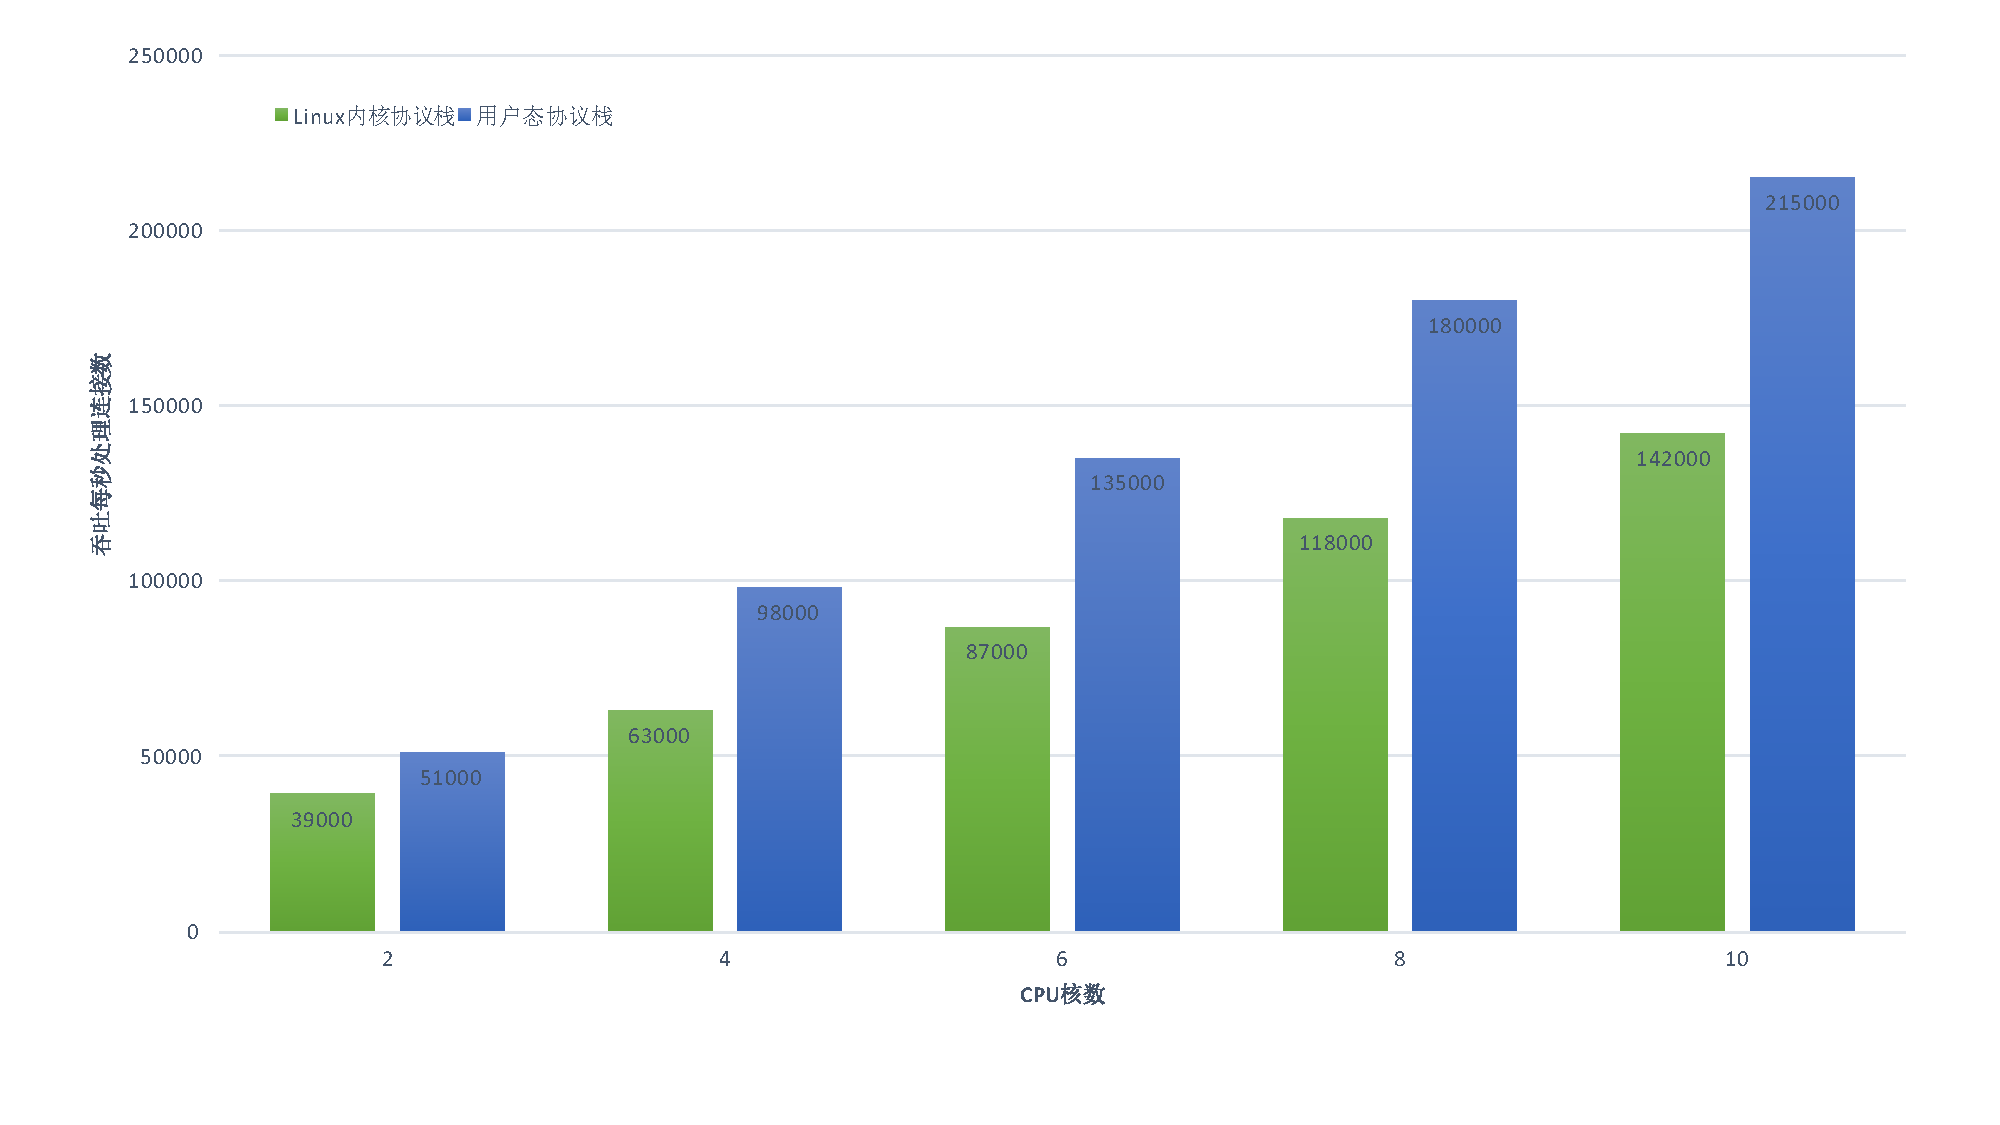
\includegraphics[width=\textwidth]{NginxRPS}
  \caption{Nginx网络吞吐性能对比图}
  \label{fig:NginxRPS}
\end{figure}
\vspace{-10pt}

\vspace{-10pt}
\begin{figure}[H] % use float package if you want it here
  \centering
  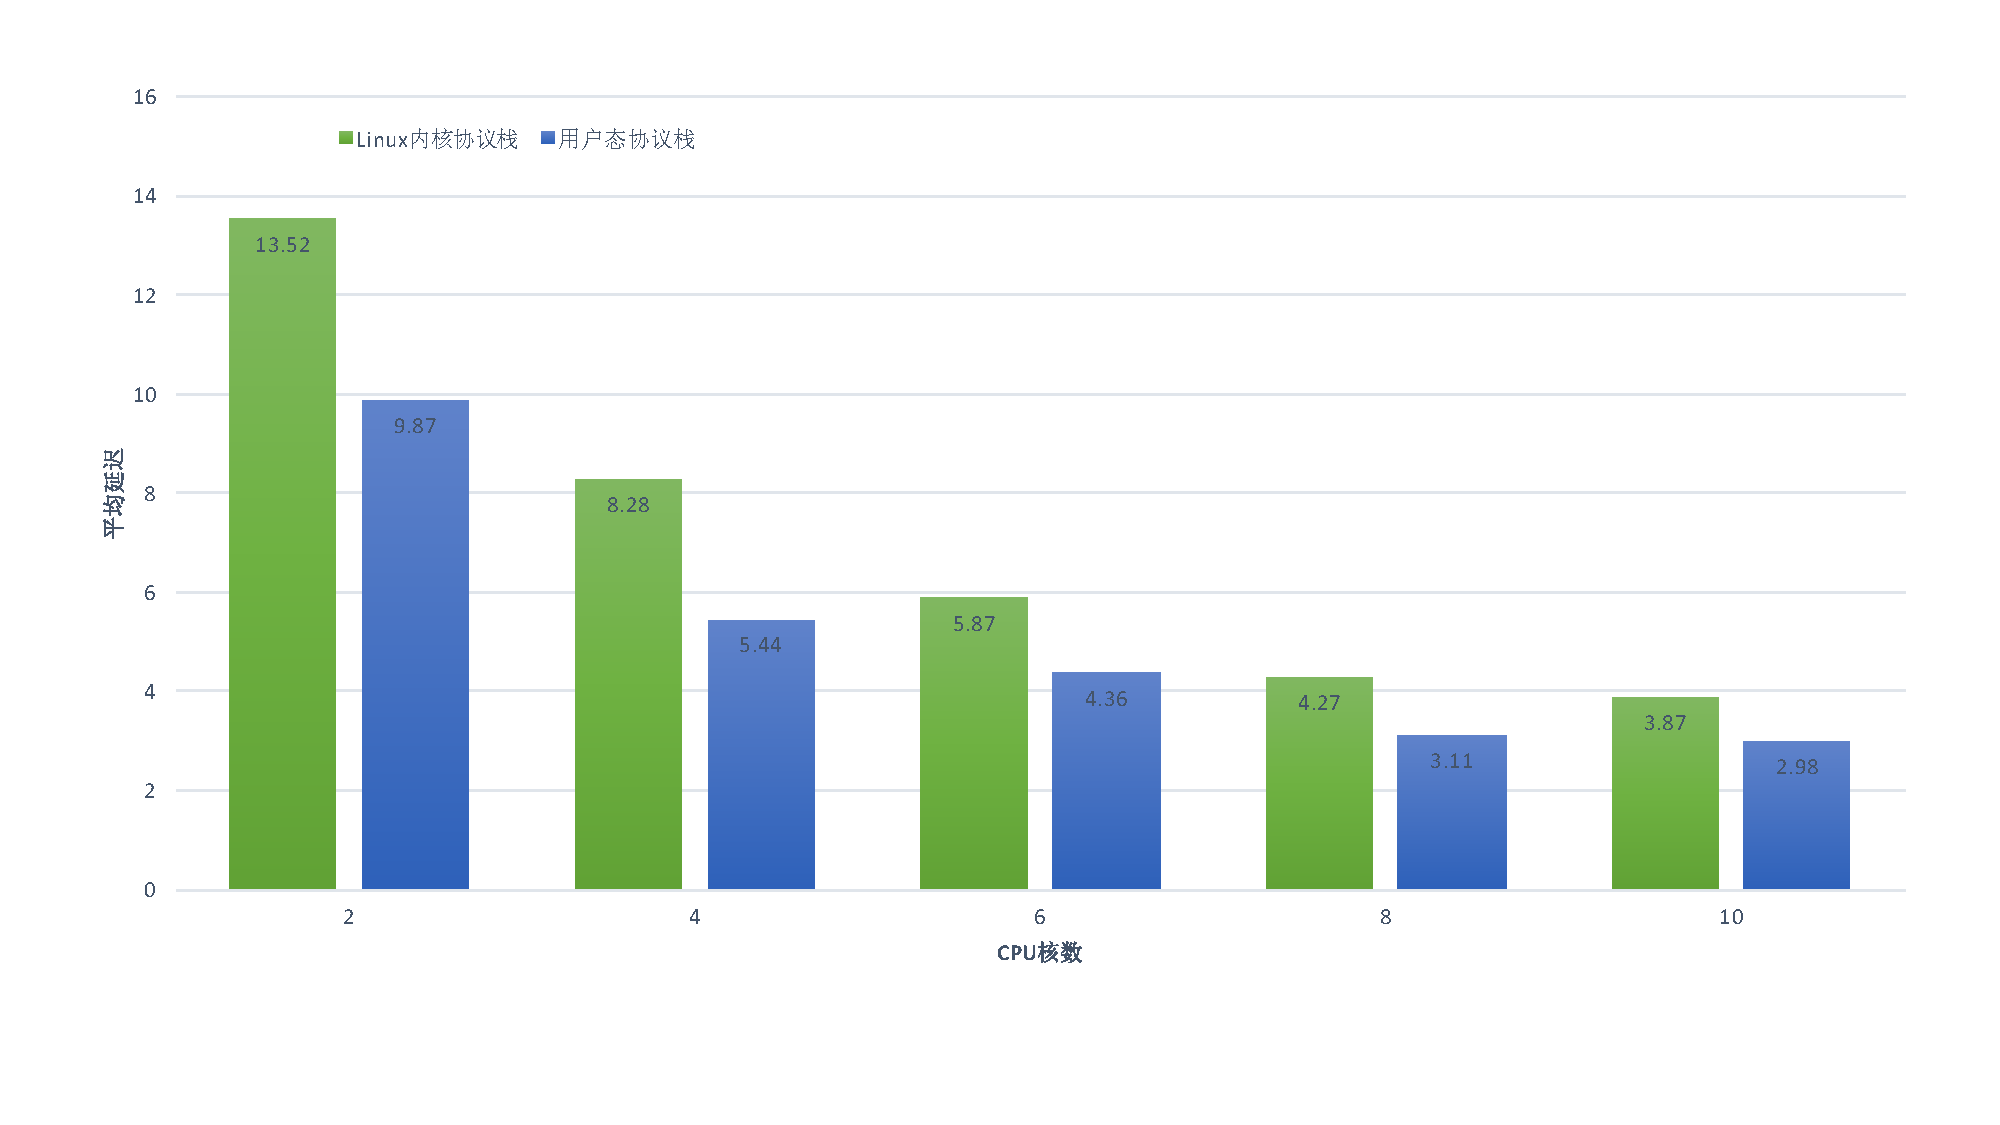
\includegraphics[width=\textwidth]{NginxAvg}
  \caption{Nginx平均延迟性能对比图}
  \label{fig:NginxAvg}
\end{figure}
\vspace{-10pt}

两图的横轴都是占用CPU的核数,纵轴分别是每秒处理连接数RPS(request per second)和平均延迟(单位是毫秒),本用户态协议栈相比Linux内核协议栈在二核、四核、六核、八核、十核下网络吞吐RPS分别提升30\%、55\%、55\%、52\%、51\%,而平均延迟分别降低27\%、34\%、25\%、27\%、22\%。网络延迟是网络服务质量中重要指标,本实验还利用wrk工具配合编写的测量延迟lua脚本,在二核的情况下对分别基于该用户态协议栈与Linux内核协议栈的Nginx网络延迟进行更加详细的统计与对比,绘制成如下延迟累积分布图~\ref{fig:NginxTail},横轴是延迟,单位是毫秒。可以看到,在99.9999\%对应的用户态协议栈延迟是24.98ms,相比内核协议栈268.5ms降低了90\%之多。尾延迟的大幅降低对于网络游戏这类延迟敏感性要求高的网络应用有着重要意义。

\vspace{-10pt}
\begin{figure}[H] % use float package if you want it here
  \centering
  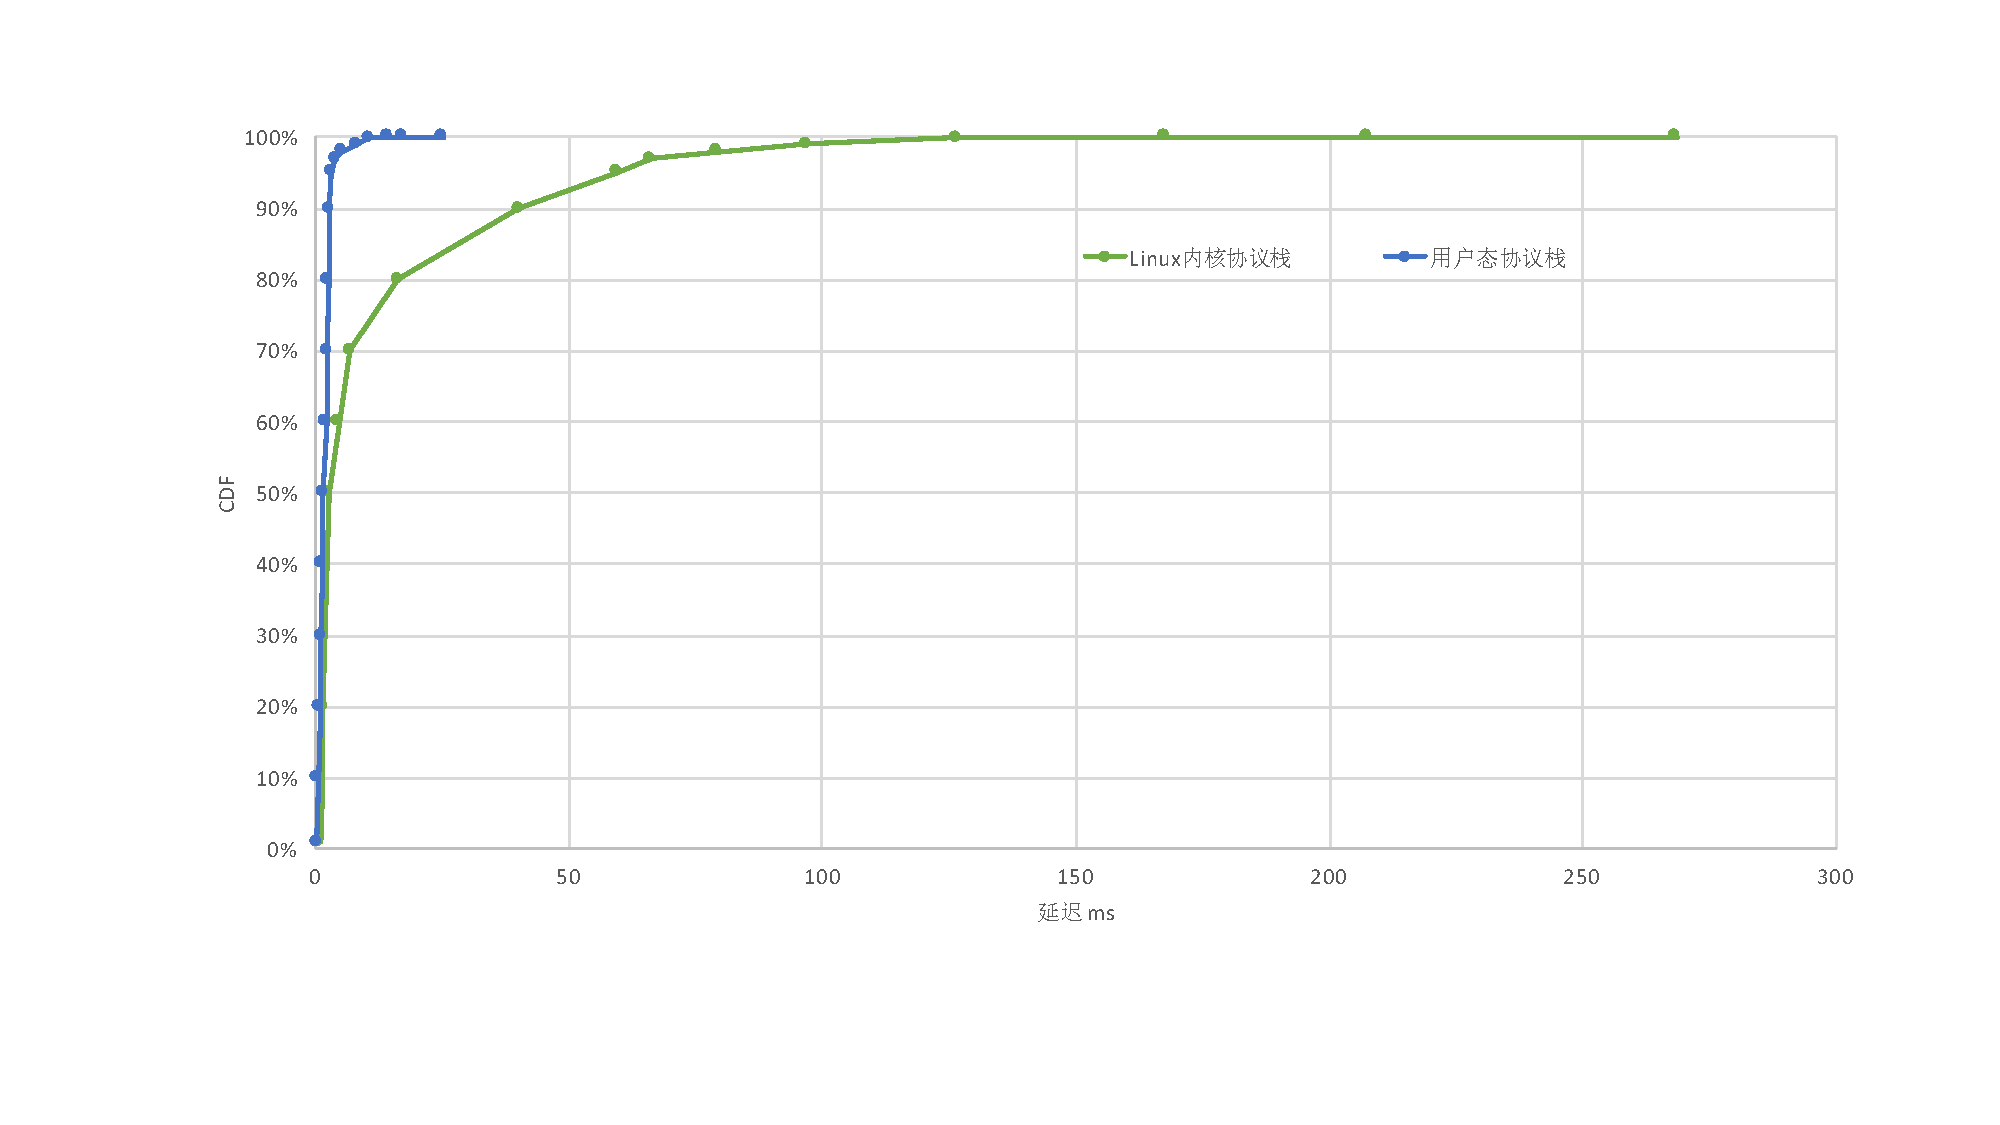
\includegraphics[width=\textwidth]{NginxTail}
  \caption{Nginx延迟累积分布图}
  \label{fig:NginxTail}
\end{figure}
\vspace{-10pt}

\section{Lighttpd实验结果}
Lighttpd相比Nginx、Apache是一个更加轻量级的Web服务器,其工作模式与Nginx类似,支持单进程模式和多进程主从模式。目前业界影响力最大并且开源的用户态协议栈mTCP已成功移植Lighttpd,为了与mTCP进行性能对比,本文将Lighttpd移植到本用户态协议栈上,移植过程中遇到的两点问题已经成功解决,第一个问题是返回给Lighttpd应用的套接字文件描述符过大从而导致数组越界访问,第二个问题是Lighttpd不像Nginx可以在配置文件中对worker进程设置亲核性,这导致Lighttpd的worker进程与协议栈进程发生严重的CPU资源争抢,这两个问题已经在兼容性设计一节中详细描述,此处不予赘述。实验依然使用wrk这款benchmark工具进行压力测试,两个客户机同时开启64个线程,512个并发连接对服务器进行压力测试,得到在双核下与Linux内核协议栈、mTCP的性能对比图如下~\ref{fig:compare},相比Linux内核协议栈性能提升37\%,不过由于本用户态协议栈运行一个worker需要占用两个核,与mTCP对比时候是其运行两个mTCP线程与两个网络应用线程,这样相比之下本用户态协议栈的性能确实只有mTCP的66\%。当然mTCP移植网络应用需要对其所有网络POSIX API进行修改,而本用户态协议栈可以在完全不需要修改任何源码的前提下为传统网络应用带来性能提升,除此之外mTCP只是简易TCP/IP协议栈,不具备UDP功能以及抵御网络安全攻击的能力较差,这也是本协议栈相比mTCP的优势。

\vspace{-10pt}
\begin{figure}[H] % use float package if you want it here
  \centering
  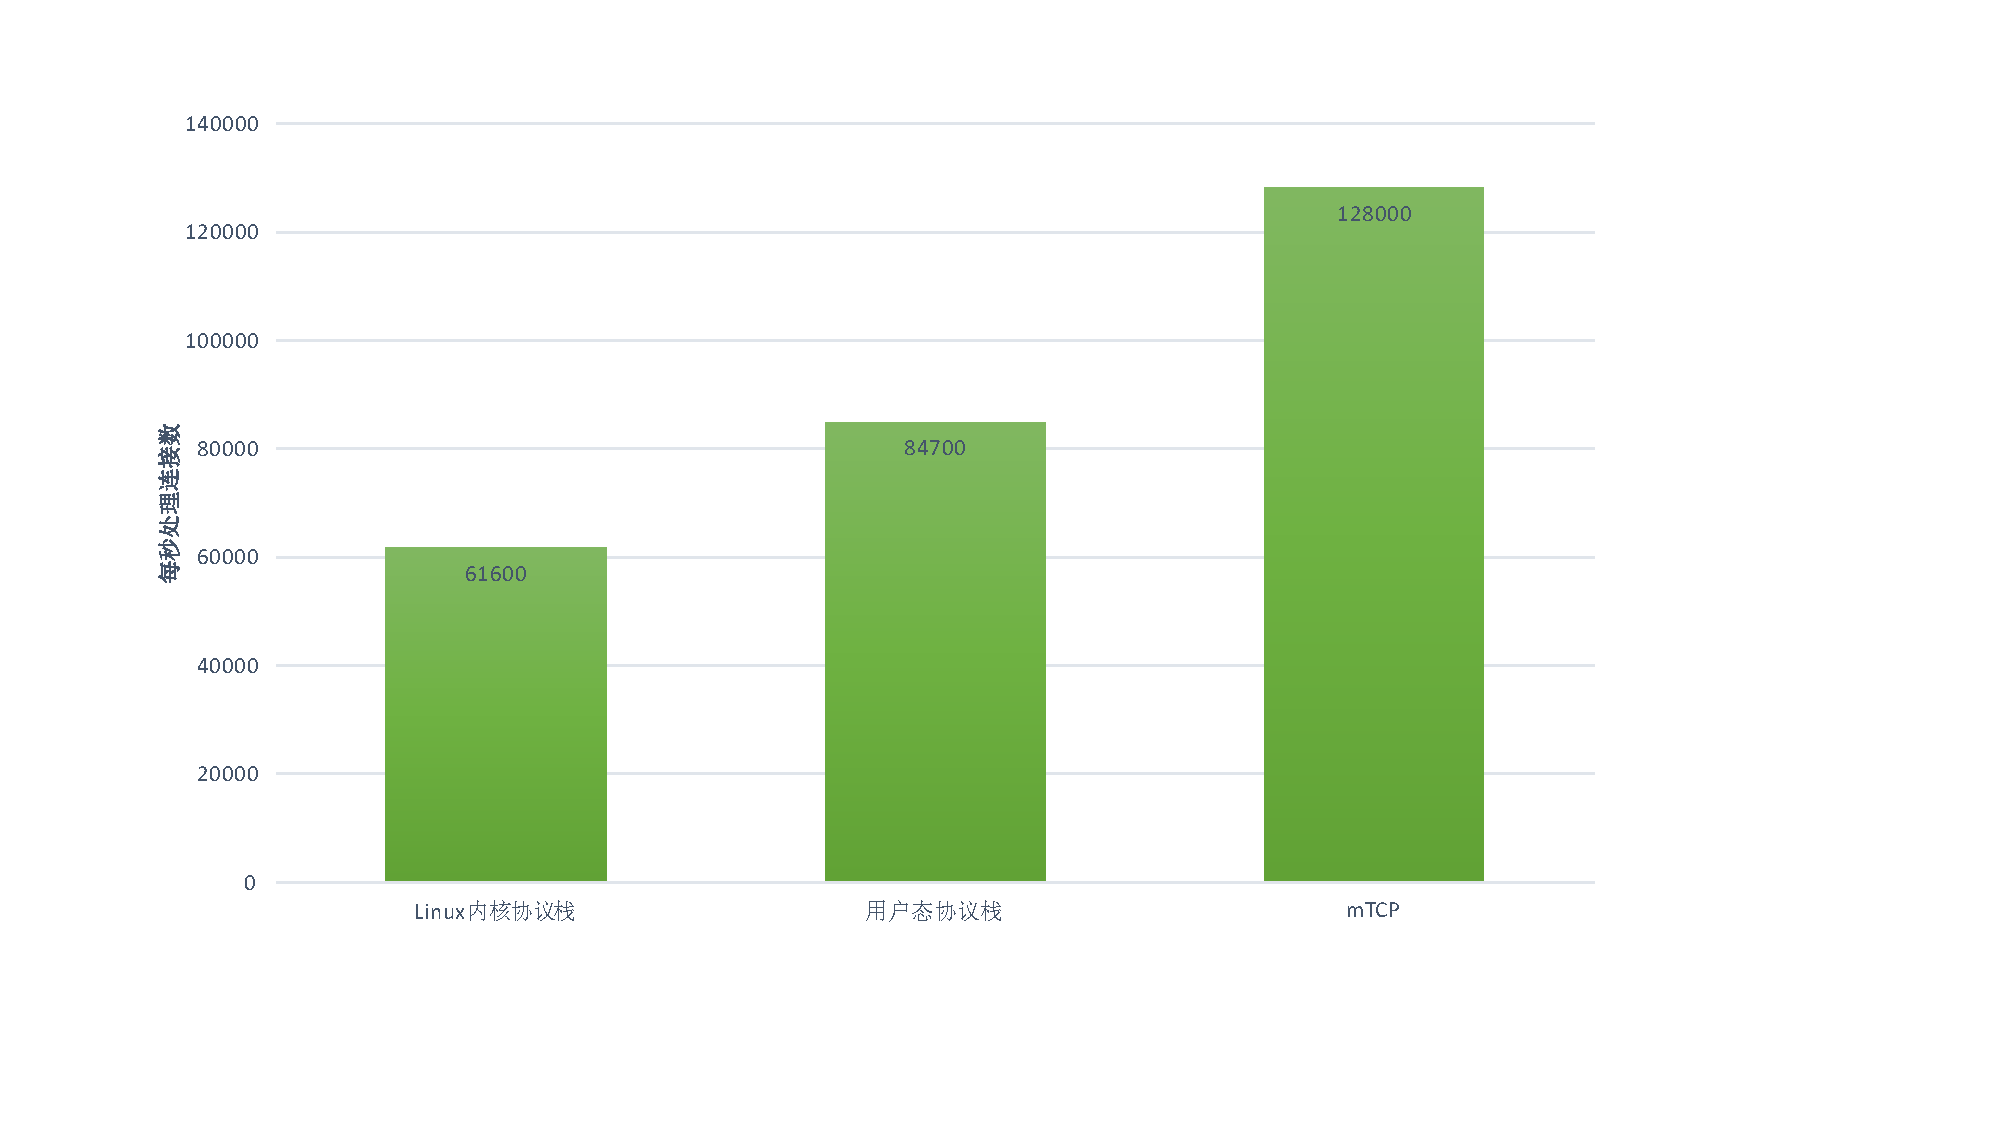
\includegraphics[width=\textwidth]{compare}
  \caption{Lighttpd性能对比图}
  \label{fig:compare}
\end{figure}
\vspace{-10pt}

\vspace{-10pt}
\begin{figure}[H] % use float package if you want it here
  \centering
  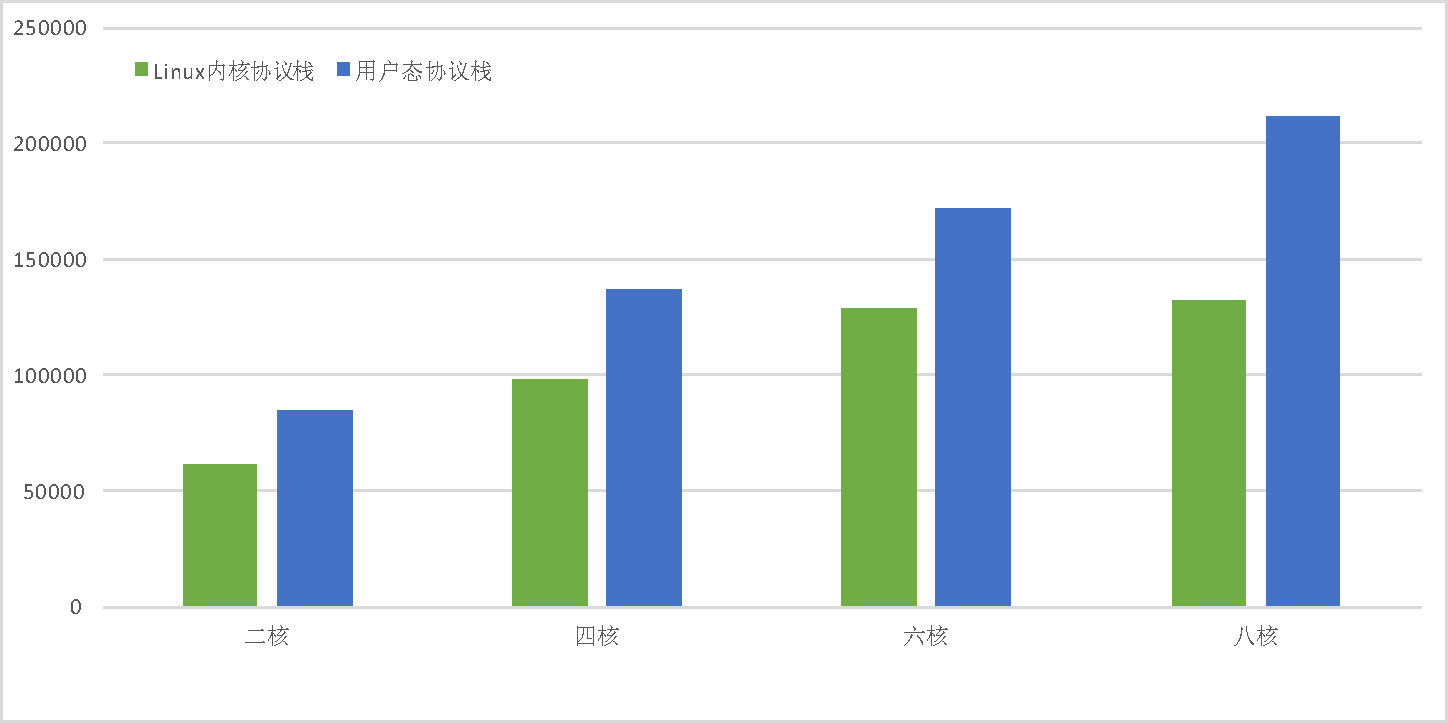
\includegraphics[width=\textwidth]{LighttpdRPS}
  \caption{Lighttpd多核性能对比图}
  \label{fig:LighttpdRPS}
\end{figure}
\vspace{-10pt}

与此同时也对Lighttpd移植后的多核吞吐性能进行实验,与Nginx实验方式一样在二核、四核、六核、八核下进行压力测试,得到如图~\ref{fig:LighttpdRPS}的多核吞吐网络性能对比图。

\section{Redis实验结果}

在内存计算领域,Key Value存储已成为分布式系统中存储共享数据结构的重要基础设施服务。在生产环境中,许多数据结构可以用一个键值哈希表来表示,例如在NoSQL数据库中的数据索引、机器学习训练中的模型参数、图形计算中的节点和边缘以及分布式同步中的序列器,这使得Redis、Memcached等Key Value内存服务器被广泛使用。当前物理内存与网卡控制器的带宽资源已经不在成为系统的性能瓶颈,内核网络协议栈就成为KV存储服务器在高并发网络环境下的性能短板。所以,本工作将Redis这款目前业界最为常用的KV内存服务器移植到该用户态协议栈上。由于Redis只有单进程一种工作模式,而如果要进行横向扩展则通常使用分布式的策略,所以本实验仅使用两个物理核对Redis基于本用户态协议栈和Linux内核协议栈进行对比,服务器端运行Redis Server进程,而在客户机中运行Redis自带的benchmark工具并在100个网络并发下进行100w次不同命令的压力测试,在此仅列举出GET、PUT两种较为常见的内存KV操作。

\vspace{-10pt}
\begin{figure}[H] % use float package if you want it here
  \centering
  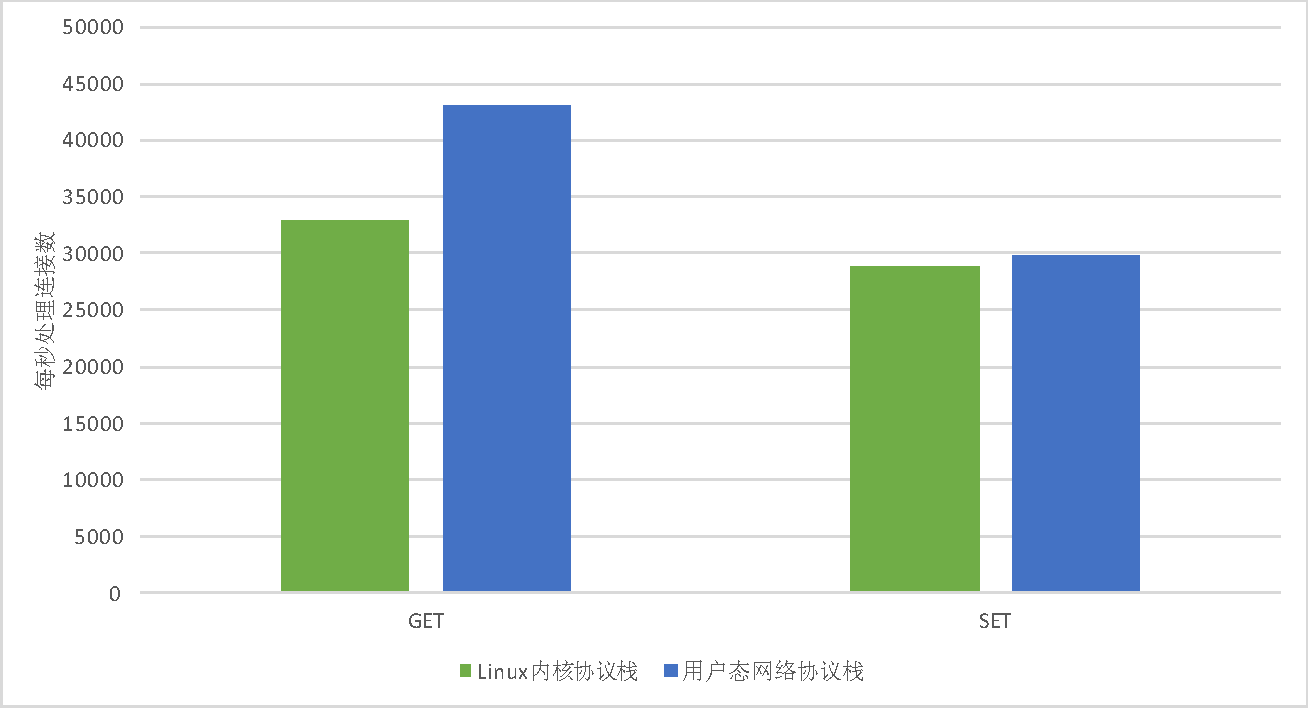
\includegraphics[width=\textwidth]{redisRPS}
  \caption{Redis性能对比图}
  \label{fig:redisRPS}
\end{figure}
\vspace{-10pt}

性能对比如~\ref{fig:redisRPS}图所示,纵轴是每秒处理连接数,可以看到用户协议栈对于GET操作有31\%较为明显的性能提升,但对于PUT等其他操作提升有限,不过KV内存服务器中众多场景的网络流量大多由GET操作构成,这种性能提升对于真实生产环境同样具有重要意义。

\section{实验结果总结与分析}

本章对已经成功移植的Nginx、Lighttpd、Redis这三款网络应用进行压力测试与性能对比分析,可以看出本用户态协议栈系统既可以达到不需要修改传统网络应用源码的高度兼容性,同时又能为传统网络应用带来较为明显的性能提升。在Nginx、Lighttpd这类Web服务器中为每秒处理连接数带来超过50\%的性能提升,并在十核之内维持着0.88的线性扩展系数。对Redis这类Key Value内存服务器的GET操作带来超过30\%的性能提升。此外,该用户态协议栈系统还移植到自行开发的传统多进程fork网络模型与基于epoll的多线程网络模型等多种网络服务器,均获得超过40\%的性能提升。
\chapter{总结与展望}
本章将对本人毕业论文相关工作进行总结与展望,总结是从当前网络协议栈兼容性方面和本用户态协议栈工作两个进行,展望是针对当前用户态协议栈系统的不足,提出几点可以在将来的研究中进行改进的设想。
\section{总结}
移动互联网和人工智能网络的兴起使得数据中心网络流量与日俱增,与此同时,在硬件设备方面网卡与物理内存带宽的飞速发展使得网络相关应用的性能瓶颈逐渐转移到传统内核网络协议栈中。学术界和工业界对网络协议栈在内核态和用户态进行了各种方式的优化,内核态网络协议栈的优化带来的性能提升有限,用户态协议栈性能较高但难以兼容现有传统网络应用,如表~\ref{tab:compare}所示,在兼容性从是否支持POSIX API、是否需要修改应用源码、是否支持Epoll等IO多路复用机制这三个方面对本工作的用户态协议栈与其他已有协议栈进行对比,可以看到本工作达到达到与Affinity-Accept、Fastsocket一样优秀的用户兼容性,并通过实验验证为Nginx等Web服务器带来的网络性能提升高于这两者。

\begin{table}[]
\centering
\caption{协议栈兼容性对比}
\label{tab:compare}
\begin{tabular}{lllp{3cm}}
\toprule[1.5pt]
\textbf{协议栈名称} & \textbf{是否支持POSIX API} & \textbf{是否需要修改应用源码} & \textbf{是否支持Epoll等IO多路复用} \\ 
\midrule[1pt]
Affinity-Accept & 是 & 不需要 & 支持 \\
MegaPipe &  否  & 需要  & 不支持 \\
Fastsocket & 是 & 不需要 & 支持 \\
mTCP & POSIX-Like & 需要 & 支持 \\
IX & 否 & 需要 & 不支持 \\
F-stack & POSIX-Like & 需要 & 支持 \\
Seastar & 否 & 需要重写应用 & 异步IO \\
\textbf{本用户态协议栈*} & 是 & 不需要 & 支持 \\
\bottomrule[1.5pt]
\end{tabular}
\end{table}

为了解决移植传统应用的兼容性,本文提出在用户态实现高性能且高度兼容性的协议栈,即传统网络应用在不需要修改任何源码的前提下就可以获得网络性能的提升。从更具体的层面上,本文在用户态协议栈的工作总结起来有如下几点:

第一,将Linux内核操作系统中网络协议栈的代码剥离出来,界定底层网卡驱动收包与网络协议栈的边界,并使用DPDK提供基于轮询IO的收发包、定时器、netdev、内存管理接口替换到原来内核协议栈中的接口,将数据包结构体sk\_buff与DPDK的mbuf整合到一起,为网络协议栈和应用提供数据缓冲支持。

第二,采用协议栈进程与网络应用进程分核的设计思路,通过DPDK提供的rte\_mempool和rte\_ring对套接字、文件描述符等资源实现资源池化管理,并进行资源预分配,减少网络高并发情况下资源不断申请、释放的性能开销。并使用有名管道和内核Epoll来实现在用户态实现Epoll相关接口以及epoll\_wait阻塞接口的唤醒机制,从而完成对IO多路复用事件通知接口。以上工作都是为在用户态实现网络应用的高度兼容性打下坚实的基础。

第三,利用LD\_PRELOAD和动态链接技术对网络应用的POSIX API进行劫持,并使用文件描述符空间预分配资源池和双向映射解决网络文件描述符和非网络文件描述符的空间分割管理问题。此外,针对当前Nginx、Lighttpd等主流网络应用服务器存在多进程等并发网络模型,对系统的CPU核资源以及执行流资源进行合理匹配,从而完成并发网络应用的支持。

第四,成功移植了Nginx、Lighttpd、Redis等主流网络应用,并将自行开发的经典网络模型服务器成功移植到本用户态协议栈上,其中包括one process per request多进程模型和基于Epoll的多线程网络模型。在Nginx、Lighttpd等Web服务器上获得超过50\%的网络性能提升,并将尾延迟降低超过90\%之多,在Redis等Key Value内存服务器上对GET操作带来超过30\%的网络性能提升,最关键是这些提升都可以在完全不需要网络应用源码的前提下直接完成。

\section{展望}

本文工作的目标是在用户态实现一个既具备高度兼容性又能带来明显网络性能提升的协议栈,解决之前高性能用户态协议栈移植网络应用成本较高的问题,达到兼容性与高性能两者的平衡。当前本用户态协议栈工作确实做到了在不需要修改源码的前提下移植网络应用,不过与mTCP等高性能协议栈相比性能不到其70\%,这也是未来本协议栈工作应该在性能方面进行更加深度的优化,以使该高度兼容的用户态协议栈具备更高的网络性能。为此,本人针对当前用户态协议栈提出如下几点改进路径:

第一,由于用户态套接字、文件描述符等大页内存资源池是多个协议栈进程共享的,这会造成rte\_ring提供的申请释放接口必须使用多生产者多消费者模式,且在高并发高吞吐流量下套接字和文件描述符资源会在多个CPU核的Cache中进行迁移,这无疑造成多进程模式下压测网络性能的降低,所以需要将套接字等资源池改变成为单个协议栈进程独享。然而由于协议栈进程通过DPDK初始化时大页内存等资源的申请只能在primary进程中进行,其他协议栈secondary进程只是获取primary申请的资源池的地址,这就导致必须将primary申请的资源池根据协议栈进程个数与资源池大小进行逻辑上的切分,即资源池中资源的申请和释放的接口会带有一个表示协议栈id的编号,而每个协议栈进程在初始化的时候都能得到自己的编号,这样在套接字资源申请时候会传递协议栈id并只能该id对应的资源池片段中申请资源,这样资源的申请与释放在协议栈进程与网络应用进程中就能按照单消费者单生产者的模式进行,减少锁竞争以及Cache迁移带来的开销。当然,该设计需要一个前提就是网络流量是较为均匀地分散到各个协议栈进程中处理,否则会造成资源池片段的使用失衡,该前提是可以通过DPDK提供的对称哈希与RSS技术来保证。

第二,当前本系统的协议栈进程只能绑定一个网络应用进程,CPU资源的利用率较低,同样运行一个协议栈执行流需要与mTCP两个协议栈执行流进行对比,这也是造成与mTCP性能对比较差的重要原因。mTCP通过pthread信号与条件变量实现在一个CPU核并发运行协议栈线程和网络应用线程,而本系统将协议栈执行流放到专用物理核上应该能为提供更强大的网络处理能力,即服务更多的网络应用并发流,所以下一步应该着手实现在对网络应用的服务质量影响较小的情况下可以让多个网络应用执行流绑定在一个协议栈进程上以及不同应用的执行流均可以绑定在同一个协议栈进程,如图~\ref{fig:distribute}所示。这就需要在用户态套接字和文件描述符资源对应的结构体中加入app\_id等字段,并用全局资源池记录下所有app\_id的相应信息,比如进程数、线程数、应用名称等。

\vspace{-10pt}
\begin{figure}[H] % use float package if you want it here
  \centering
  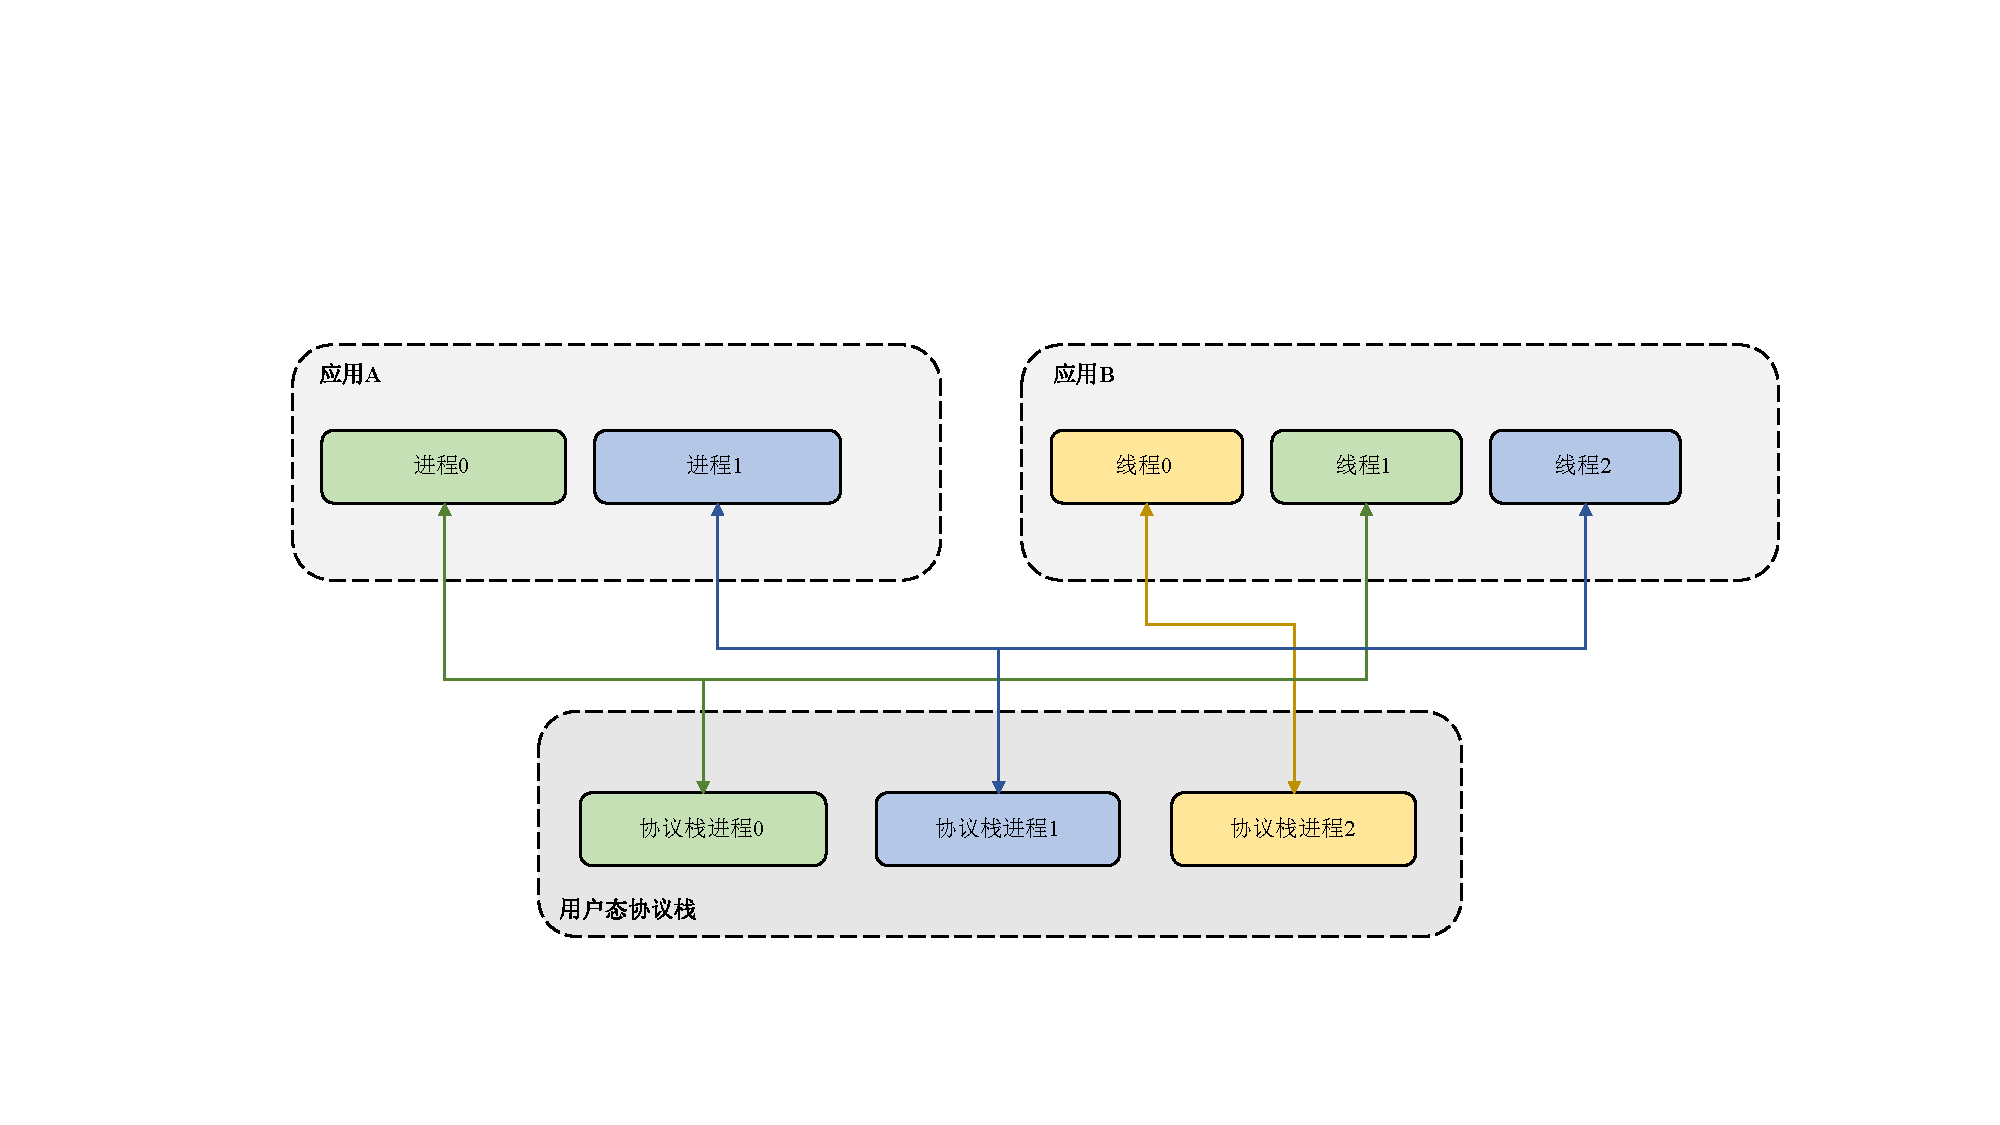
\includegraphics[width=\textwidth]{distribute}
  \caption{协议栈进程与网络执行流调度设计图}
  \label{fig:distribute}
\end{figure}
\vspace{-10pt}

第三,前两点长期稳定运行的前提需要协议栈进程本身的鲁棒性,若协议栈进程崩溃且网络应用未被通知的情况下会出现无法服务或绑定失败的异常情况,这需要系统对协议栈进程本身的运行状况进行监控。当前系统通过在协议栈primary进程建立Unix域socket而网络应用进程对其进行Unix域socket连接的方式并结合内核Epoll来完成对应用进程的异常状态的监控,若协议栈primary进程自身异常退出导致此方法无法对协议栈进程异常进行监控,所以需要将监控程序单独剥离出成为一个独立进程,该监控进程完成Unix域监听socket的建立,并在协议栈进程和网络应用进程初始化时都通过内核套接字对监控进程的Unix域监听套接字进行连接,这样当协议栈进程或应用进程异常退出后都能在监控进程中通过Epoll事件获取,此外监控进程通过内核epoll\_wait监听阻塞后并不占用CPU资源,这样所有系统监控的工作全部可以放入该监控进程模块来完成,实现系统各个模块的解耦。


%%% 其它部分
\backmatter

%% 本科生要这几个索引,研究生不要。选择性留下。
% 插图索引
%\listoffigures
% 表格索引
%\listoftables
% 公式索引
%\listofequations


%% 参考文献
% 注意:至少需要引用一篇参考文献,否则下面两行可能引起编译错误。
% 如果不需要参考文献,请将下面两行删除或注释掉。
% 数字式引用
\bibliographystyle{thuthesis-numeric}
% 作者-年份式引用
%\bibliographystyle{thuthesis}
\bibliography{ref/refs}


%% 致谢
% 如果使用声明扫描页,将可选参数指定为扫描后的 PDF 文件名,例如:
% \begin{acknowledgement}[scan-statement.pdf]
\begin{acknowledgement}
感谢我的导师李丹副教授在这几年的研究生生涯中给予本人的指导。感谢清华计算机系NASP实验室提供的良好的科研工作环境。

感谢我的父母和女朋友一直以来对我的关心与照顾。感谢实验室的陈聪捷师兄、王方鑫师兄、令瑞林师兄、黄昱恺师兄、李俊峰师兄、林督师兄、耿金坤同学、程阳同学在研究生期间中给我提供的建议和帮助。

最后,忠心感谢美丽的清华为我提供丰富的文化体育氛围与齐全的基础设施,在清华园这几年的时光将是我人生中美好的回忆,愿母校越来越强大。

\end{acknowledgement}


%% 附录
%%\begin{appendix}
%%\chapter{外文资料原文}
\label{cha:engorg}

\title{The title of the English paper}

\textbf{Abstract:} As one of the most widely used techniques in operations
research, \emph{ mathematical programming} is defined as a means of maximizing a
quantity known as \emph{bjective function}, subject to a set of constraints
represented by equations and inequalities. Some known subtopics of mathematical
programming are linear programming, nonlinear programming, multiobjective
programming, goal programming, dynamic programming, and multilevel
programming$^{[1]}$.

It is impossible to cover in a single chapter every concept of mathematical
programming. This chapter introduces only the basic concepts and techniques of
mathematical programming such that readers gain an understanding of them
throughout the book$^{[2,3]}$.


\section{Single-Objective Programming}
The general form of single-objective programming (SOP) is written
as follows,
\begin{equation}\tag*{(123)} % 如果附录中的公式不想让它出现在公式索引中,那就请
                             % 用 \tag*{xxxx}
\left\{\begin{array}{l}
\max \,\,f(x)\\[0.1 cm]
\mbox{subject to:} \\ [0.1 cm]
\qquad g_j(x)\le 0,\quad j=1,2,\cdots,p
\end{array}\right.
\end{equation}
which maximizes a real-valued function $f$ of
$x=(x_1,x_2,\cdots,x_n)$ subject to a set of constraints.

\newtheorem{mpdef}{Definition}[chapter]
\begin{mpdef}
In SOP, we call $x$ a decision vector, and
$x_1,x_2,\cdots,x_n$ decision variables. The function
$f$ is called the objective function. The set
\begin{equation}\tag*{(456)} % 这里同理,其它不再一一指定。
S=\left\{x\in\Re^n\bigm|g_j(x)\le 0,\,j=1,2,\cdots,p\right\}
\end{equation}
is called the feasible set. An element $x$ in $S$ is called a
feasible solution.
\end{mpdef}

\newtheorem{mpdefop}[mpdef]{Definition}
\begin{mpdefop}
A feasible solution $x^*$ is called the optimal
solution of SOP if and only if
\begin{equation}
f(x^*)\ge f(x)
\end{equation}
for any feasible solution $x$.
\end{mpdefop}

One of the outstanding contributions to mathematical programming was known as
the Kuhn-Tucker conditions\ref{eq:ktc}. In order to introduce them, let us give
some definitions. An inequality constraint $g_j(x)\le 0$ is said to be active at
a point $x^*$ if $g_j(x^*)=0$. A point $x^*$ satisfying $g_j(x^*)\le 0$ is said
to be regular if the gradient vectors $\nabla g_j(x)$ of all active constraints
are linearly independent.

Let $x^*$ be a regular point of the constraints of SOP and assume that all the
functions $f(x)$ and $g_j(x),j=1,2,\cdots,p$ are differentiable. If $x^*$ is a
local optimal solution, then there exist Lagrange multipliers
$\lambda_j,j=1,2,\cdots,p$ such that the following Kuhn-Tucker conditions hold,
\begin{equation}
\label{eq:ktc}
\left\{\begin{array}{l}
    \nabla f(x^*)-\sum\limits_{j=1}^p\lambda_j\nabla g_j(x^*)=0\\[0.3cm]
    \lambda_jg_j(x^*)=0,\quad j=1,2,\cdots,p\\[0.2cm]
    \lambda_j\ge 0,\quad j=1,2,\cdots,p.
\end{array}\right.
\end{equation}
If all the functions $f(x)$ and $g_j(x),j=1,2,\cdots,p$ are convex and
differentiable, and the point $x^*$ satisfies the Kuhn-Tucker conditions
(\ref{eq:ktc}), then it has been proved that the point $x^*$ is a global optimal
solution of SOP.

\subsection{Linear Programming}
\label{sec:lp}

If the functions $f(x),g_j(x),j=1,2,\cdots,p$ are all linear, then SOP is called
a {\em linear programming}.

The feasible set of linear is always convex. A point $x$ is called an extreme
point of convex set $S$ if $x\in S$ and $x$ cannot be expressed as a convex
combination of two points in $S$. It has been shown that the optimal solution to
linear programming corresponds to an extreme point of its feasible set provided
that the feasible set $S$ is bounded. This fact is the basis of the {\em simplex
  algorithm} which was developed by Dantzig as a very efficient method for
solving linear programming.
\begin{table}[ht]
\centering
  \centering
  \caption*{Table~1\hskip1em This is an example for manually numbered table, which
    would not appear in the list of tables}
  \label{tab:badtabular2}
  \begin{tabular}[c]{|m{1.5cm}|c|c|c|c|c|c|}\hline
    \multicolumn{2}{|c|}{Network Topology} & \# of nodes &
    \multicolumn{3}{c|}{\# of clients} & Server \\\hline
    GT-ITM & Waxman Transit-Stub & 600 &
    \multirow{2}{2em}{2\%}&
    \multirow{2}{2em}{10\%}&
    \multirow{2}{2em}{50\%}&
    \multirow{2}{1.2in}{Max. Connectivity}\\\cline{1-3}
    \multicolumn{2}{|c|}{Inet-2.1} & 6000 & & & &\\\hline
    \multirow{2}{1.5cm}{Xue} & Rui  & Ni &\multicolumn{4}{c|}{\multirow{2}*{\thuthesis}}\\\cline{2-3}
    & \multicolumn{2}{c|}{ABCDEF} &\multicolumn{4}{c|}{} \\\hline
\end{tabular}
\end{table}

Roughly speaking, the simplex algorithm examines only the extreme points of the
feasible set, rather than all feasible points. At first, the simplex algorithm
selects an extreme point as the initial point. The successive extreme point is
selected so as to improve the objective function value. The procedure is
repeated until no improvement in objective function value can be made. The last
extreme point is the optimal solution.

\subsection{Nonlinear Programming}

If at least one of the functions $f(x),g_j(x),j=1,2,\cdots,p$ is nonlinear, then
SOP is called a {\em nonlinear programming}.

A large number of classical optimization methods have been developed to treat
special-structural nonlinear programming based on the mathematical theory
concerned with analyzing the structure of problems.
\begin{figure}[h]
  \centering
  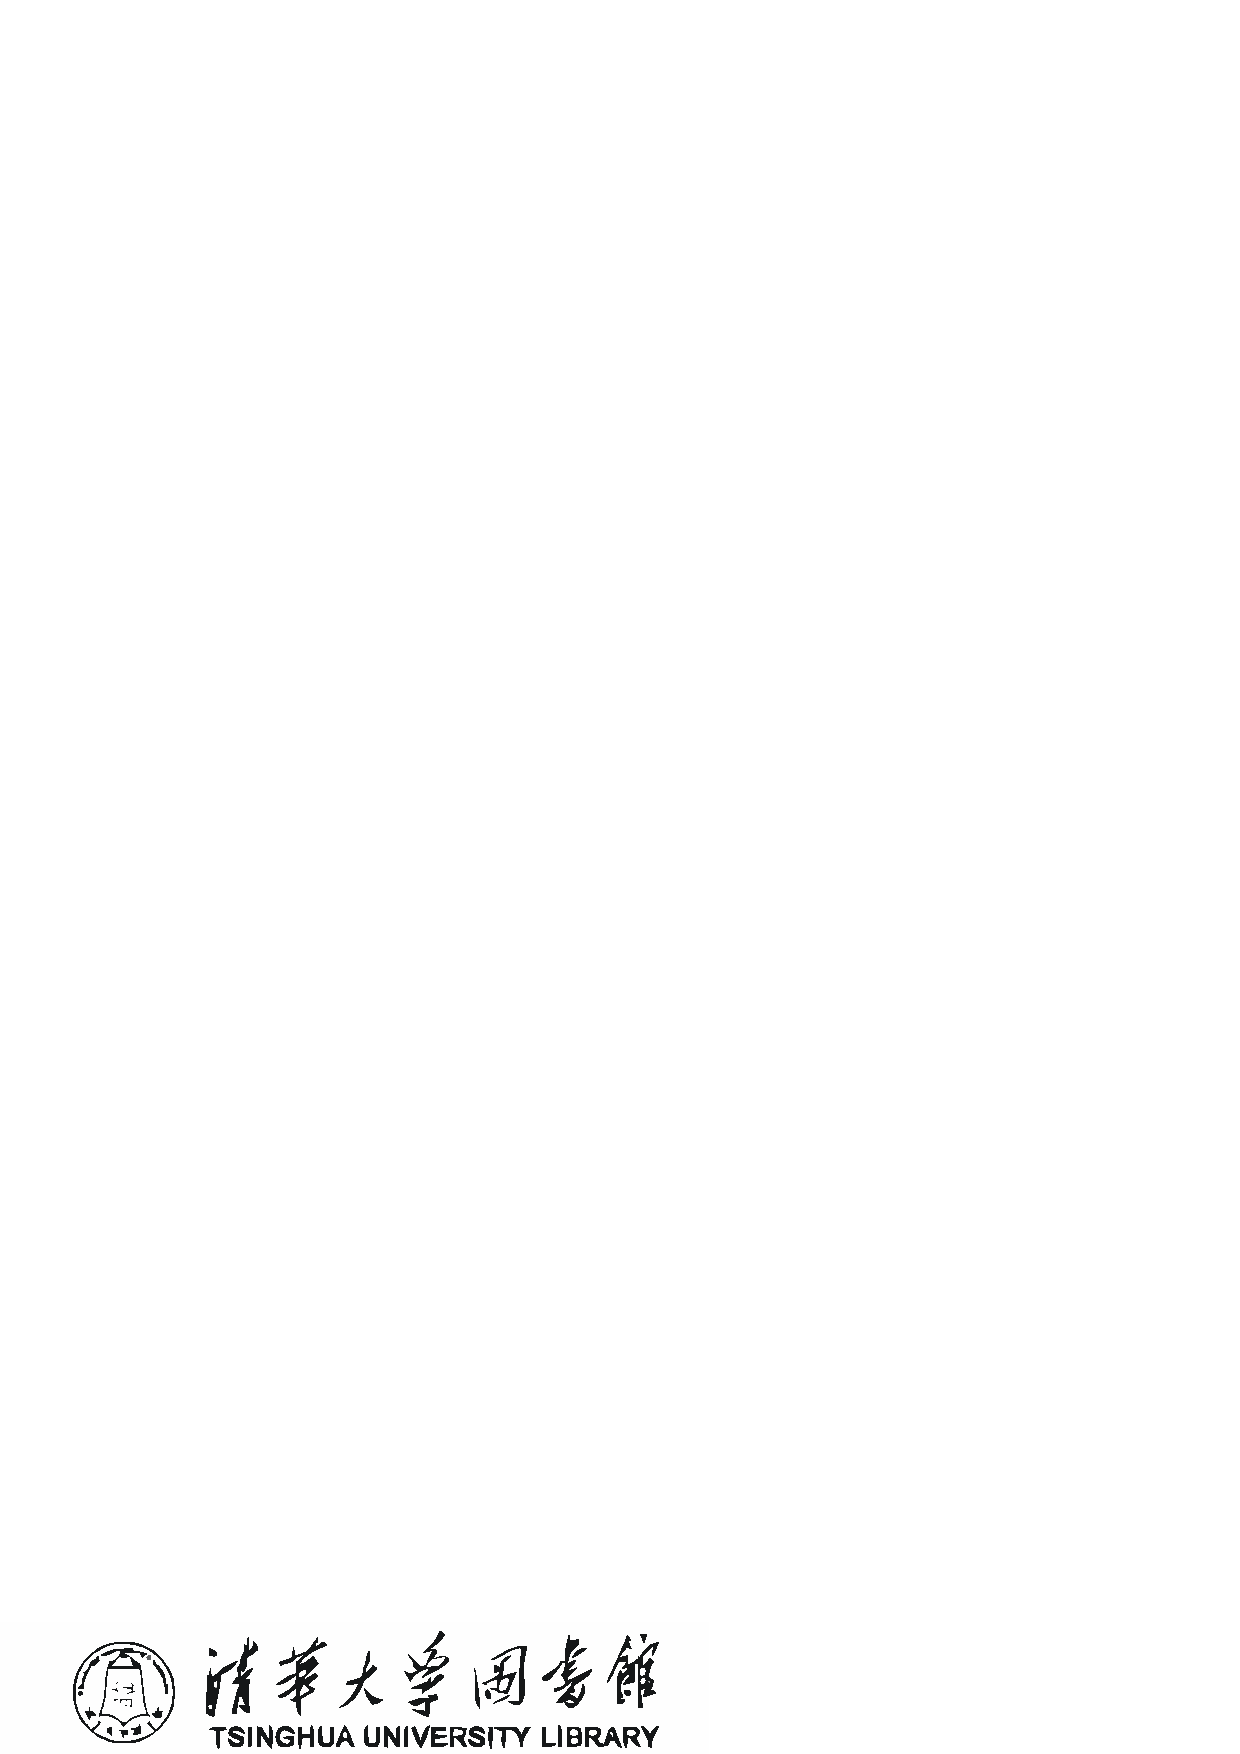
\includegraphics{thu-lib-logo}
  \caption*{Figure~1\quad This is an example for manually numbered figure,
    which would not appear in the list of figures}
  \label{tab:badfigure2}
\end{figure}

Now we consider a nonlinear programming which is confronted solely with
maximizing a real-valued function with domain $\Re^n$.  Whether derivatives are
available or not, the usual strategy is first to select a point in $\Re^n$ which
is thought to be the most likely place where the maximum exists. If there is no
information available on which to base such a selection, a point is chosen at
random. From this first point an attempt is made to construct a sequence of
points, each of which yields an improved objective function value over its
predecessor. The next point to be added to the sequence is chosen by analyzing
the behavior of the function at the previous points. This construction continues
until some termination criterion is met. Methods based upon this strategy are
called {\em ascent methods}, which can be classified as {\em direct methods},
{\em gradient methods}, and {\em Hessian methods} according to the information
about the behavior of objective function $f$. Direct methods require only that
the function can be evaluated at each point. Gradient methods require the
evaluation of first derivatives of $f$. Hessian methods require the evaluation
of second derivatives. In fact, there is no superior method for all
problems. The efficiency of a method is very much dependent upon the objective
function.

\subsection{Integer Programming}

{\em Integer programming} is a special mathematical programming in which all of
the variables are assumed to be only integer values. When there are not only
integer variables but also conventional continuous variables, we call it {\em
  mixed integer programming}. If all the variables are assumed either 0 or 1,
then the problem is termed a {\em zero-one programming}. Although integer
programming can be solved by an {\em exhaustive enumeration} theoretically, it
is impractical to solve realistically sized integer programming problems. The
most successful algorithm so far found to solve integer programming is called
the {\em branch-and-bound enumeration} developed by Balas (1965) and Dakin
(1965). The other technique to integer programming is the {\em cutting plane
  method} developed by Gomory (1959).

\hfill\textit{Uncertain Programming\/}\quad(\textsl{BaoDing Liu, 2006.2})

\section*{References}
\noindent{\itshape NOTE: These references are only for demonstration. They are
  not real citations in the original text.}

\begin{translationbib}
\item Donald E. Knuth. The \TeX book. Addison-Wesley, 1984. ISBN: 0-201-13448-9
\item Paul W. Abrahams, Karl Berry and Kathryn A. Hargreaves. \TeX\ for the
  Impatient. Addison-Wesley, 1990. ISBN: 0-201-51375-7
\item David Salomon. The advanced \TeX book.  New York : Springer, 1995. ISBN:0-387-94556-3
\end{translationbib}

\chapter{外文资料的调研阅读报告或书面翻译}

\title{英文资料的中文标题}

{\heiti 摘要:} 本章为外文资料翻译内容。如果有摘要可以直接写上来,这部分好像没有
明确的规定。

\section{单目标规划}
北冥有鱼,其名为鲲。鲲之大,不知其几千里也。化而为鸟,其名为鹏。鹏之背,不知其几
千里也。怒而飞,其翼若垂天之云。是鸟也,海运则将徙于南冥。南冥者,天池也。
\begin{equation}\tag*{(123)}
 p(y|\mathbf{x}) = \frac{p(\mathbf{x},y)}{p(\mathbf{x})}=
\frac{p(\mathbf{x}|y)p(y)}{p(\mathbf{x})}
\end{equation}

吾生也有涯,而知也无涯。以有涯随无涯,殆已!已而为知者,殆而已矣!为善无近名,为
恶无近刑,缘督以为经,可以保身,可以全生,可以养亲,可以尽年。

\subsection{线性规划}
庖丁为文惠君解牛,手之所触,肩之所倚,足之所履,膝之所倚,砉然响然,奏刀騞然,莫
不中音,合于桑林之舞,乃中经首之会。
\begin{table}[ht]
\centering
  \centering
  \caption*{表~1\hskip1em 这是手动编号但不出现在索引中的一个表格例子}
  \label{tab:badtabular3}
  \begin{tabular}[c]{|m{1.5cm}|c|c|c|c|c|c|}\hline
    \multicolumn{2}{|c|}{Network Topology} & \# of nodes &
    \multicolumn{3}{c|}{\# of clients} & Server \\\hline
    GT-ITM & Waxman Transit-Stub & 600 &
    \multirow{2}{2em}{2\%}&
    \multirow{2}{2em}{10\%}&
    \multirow{2}{2em}{50\%}&
    \multirow{2}{1.2in}{Max. Connectivity}\\\cline{1-3}
    \multicolumn{2}{|c|}{Inet-2.1} & 6000 & & & &\\\hline
    \multirow{2}{1.5cm}{Xue} & Rui  & Ni &\multicolumn{4}{c|}{\multirow{2}*{\thuthesis}}\\\cline{2-3}
    & \multicolumn{2}{c|}{ABCDEF} &\multicolumn{4}{c|}{} \\\hline
\end{tabular}
\end{table}

文惠君曰:“嘻,善哉!技盖至此乎?”庖丁释刀对曰:“臣之所好者道也,进乎技矣。始臣之
解牛之时,所见无非全牛者;三年之后,未尝见全牛也;方今之时,臣以神遇而不以目视,
官知止而神欲行。依乎天理,批大郤,导大窾,因其固然。技经肯綮之未尝,而况大坬乎!
良庖岁更刀,割也;族庖月更刀,折也;今臣之刀十九年矣,所解数千牛矣,而刀刃若新发
于硎。彼节者有间而刀刃者无厚,以无厚入有间,恢恢乎其于游刃必有余地矣。是以十九年
而刀刃若新发于硎。虽然,每至于族,吾见其难为,怵然为戒,视为止,行为迟,动刀甚微,
謋然已解,如土委地。提刀而立,为之而四顾,为之踌躇满志,善刀而藏之。”

文惠君曰:“善哉!吾闻庖丁之言,得养生焉。”


\subsection{非线性规划}
孔子与柳下季为友,柳下季之弟名曰盗跖。盗跖从卒九千人,横行天下,侵暴诸侯。穴室枢
户,驱人牛马,取人妇女。贪得忘亲,不顾父母兄弟,不祭先祖。所过之邑,大国守城,小
国入保,万民苦之。孔子谓柳下季曰:“夫为人父者,必能诏其子;为人兄者,必能教其弟。
若父不能诏其子,兄不能教其弟,则无贵父子兄弟之亲矣。今先生,世之才士也,弟为盗
跖,为天下害,而弗能教也,丘窃为先生羞之。丘请为先生往说之。”
\begin{figure}[h]
  \centering
  
\includegraphics{thu-whole-logo}
  \caption*{图~1\hskip1em 这是手动编号但不出现索引中的图片的例子}
  \label{tab:badfigure3}
\end{figure}

柳下季曰:“先生言为人父者必能诏其子,为人兄者必能教其弟,若子不听父之诏,弟不受
兄之教,虽今先生之辩,将奈之何哉?且跖之为人也,心如涌泉,意如飘风,强足以距敌,
辩足以饰非。顺其心则喜,逆其心则怒,易辱人以言。先生必无往。”

孔子不听,颜回为驭,子贡为右,往见盗跖。

\subsection{整数规划}
盗跖乃方休卒徒大山之阳,脍人肝而餔之。孔子下车而前,见谒者曰:“鲁人孔丘,闻将军
高义,敬再拜谒者。”谒者入通。盗跖闻之大怒,目如明星,发上指冠,曰:“此夫鲁国之
巧伪人孔丘非邪?为我告之:尔作言造语,妄称文、武,冠枝木之冠,带死牛之胁,多辞缪
说,不耕而食,不织而衣,摇唇鼓舌,擅生是非,以迷天下之主,使天下学士不反其本,妄
作孝弟,而侥幸于封侯富贵者也。子之罪大极重,疾走归!不然,我将以子肝益昼餔之膳。”


\chapter{其它附录}
前面两个附录主要是给本科生做例子。其它附录的内容可以放到这里,当然如果你愿意,可
以把这部分也放到独立的文件中,然后将其 \cs{input} 到主文件中。

%%\end{appendix}

%% 个人简历
\begin{resume}

  \resumeitem{个人简历}

  1994 年 10 月 8 日出生于 吉林 省 延边朝鲜族自治 州 汪清 县。

  2012 年 9 月考入 北京邮电 大学 信息与通信工程 学院 电子信息工程 专业,2016 年 7 月本科毕业并获得 工学 学士学位。

  2016 年 9 月推荐免试进入 清华 大学 计算机科学与技术 系攻读 硕士 学位至今。

  \researchitem{学术论文与研究成果} % 发表的和录用的合在一起

  % 1. 已经刊载的学术论文(本人是第一作者,或者导师为第一作者本人是第二作者)
  \begin{publications}
  
  \end{publications}

  % 2. 尚未刊载,但已经接到正式录用函的学术论文(本人为第一作者,或者
  %    导师为第一作者本人是第二作者)。
  \begin{publications}[before=\publicationskip,after=\publicationskip]
    \item \textbf{姜惠友},李峻峰,李丹. 高性能网络协议栈的兼容性研究. 电信科学(已发表.2019,35(5):25-31. 中文核心期刊.)
    % \item Dan Li, \textbf{Du Lin}, Changlin Jiang. SOPA: A Packet-level Multi-path Routing Scheme in Data Center Networks. ZTE Communications,2018,(04). (已录用) 
  \end{publications}

  % 3. 其他学术论文。可列出除上述两种情况以外的其他学术论文,但必须是
  %    已经刊载或者收到正式录用函的论文。
  \begin{publications}
    % \item Yukai Huang, Jinkun Geng, \textbf{Du Lin}, Bin Wang, Junfeng Li, Ruilin Ling, Dan Li. LOS: A High Performance and Compatible User-level Network Operating System. APNet 2017 Conference.
  \end{publications}

\end{resume}


%% 本科生进行格式审查是需要下面这个表格,答辩可能不需要。选择性留下。
% 综合论文训练记录表
%\includepdf[pages=-]{scan-record.pdf}
\end{document}
